\documentclass[12pt, twoside, a4paper]{report}
\usepackage{parskip}
\usepackage[english]{babel}
\usepackage[utf8]{inputenc}
\usepackage{amsmath}
\usepackage{amssymb}
\usepackage{graphicx}
\usepackage{mathtools}
\usepackage{units}
\usepackage[margin=1.0in]{geometry}
\usepackage{comment} 
\usepackage{subcaption}
\usepackage{float}
\usepackage{units}
\usepackage{natbib}
\usepackage{multirow}
\usepackage{url}
\usepackage{amsthm}
\usepackage[ruled,vlined]{algorithm2e}
\usepackage{xfrac}
\usepackage{multirow}
\usepackage{epstopdf}
\usepackage{fancyhdr}
\usepackage{titling}
\usepackage{afterpage}
\usepackage[font=small,labelfont=it]{caption}
\usepackage{tikz}
\usepackage{subcaption}
\usepackage{setspace}
\usepackage{chemfig}
\usetikzlibrary{arrows, arrows.meta, shapes.geometric,  positioning, calc, trees, chains, decorations.pathreplacing, decorations.pathmorphing, shapes, 
matrix, shapes.symbols}

\tikzstyle{arrow} = [thick,->,>=stealth, text width=5em, text centered]
\tikzstyle{node} = [rectangle, rounded corners, thick, minimum width=2cm, minimum height=1cm,text centered,text width=3cm, draw=black]

\tikzstyle{doublearr}=[latex-latex, black, line width=0.5pt]

\tikzset{
>=stealth',
  punktchain/.style={
    rectangle, 
    rounded corners, 
    % fill=black!10,
    draw=black, very thick,
    text width=10em, 
    minimum height=3em, 
    text centered, 
    on chain},
  line/.style={draw, thick, <-},
  element/.style={
    tape,
    top color=white,
    bottom color=blue!50!black!60!,
    minimum width=8em,
    draw=blue!40!black!90, very thick,
    text width=10em, 
    minimum height=3.5em, 
    text centered, 
    on chain},
  every join/.style={->, thick,shorten >=1pt},
  decoration={brace},
  tuborg/.style={decorate},
  tubnode/.style={midway, right=2pt},
}

\newcommand\blankpage{%
    \null
    \thispagestyle{empty}%
    \addtocounter{page}{-1}%
    \newpage}


\pagestyle{fancy}
\fancyhf{}
\fancyhead[RE,LO]{\nouppercase{\rightmark}}
\fancyfoot[C]{\thepage}

\def\vec{\boldsymbol}
\def\var{\text{var}}
\DeclareMathOperator*{\argmax}{arg\,max}
\newcommand{\secref}[1]{\S\ref{#1}}

\newtheorem{definition}{Definition}[subsection]


\title{MEng Individual Project (JMC)}

\author{Daren Sin \\  Supervisor: Dr. Panos Parpas}

\date{\today}


\begin{document}

\begin{titlingpage}

\vspace*{1.5cm}

\begin{center}

\includegraphics[height=3cm]{images/imperial}
\end{center}

\vspace{1.5cm}
\begin{center}
\Large

\textsc{Department of Computing}
\end{center}

\vspace{2cm}

\begin{center}
\Large \textsc{\thetitle}

\vspace{2cm}

\textsc{\textbf{Feature selection methods in the context of epigenetics and schizophrenia}}

\end{center}

\vspace{2cm}

\begin{center}
\large \textit{Author:} \textsc{Daren Sin}

\textit{Supervisor:} \textsc{Dr. Panos Parpas}

\textit{Second marker:} \textsc{Dr. Ruth Misener}
\end{center}

\vspace{2cm}

\begin{center}
\normalsize \textsc{\thedate}
\end{center}

\end{titlingpage}

\pagenumbering{roman}

\afterpage{\blankpage}

\singlespacing
\chapter*{Abstract}
Schizophrenia is a mental disorder that is commonly perceived to be hereditary. However, there have been cases where patients with schizophrenia do not have a family member with the disorder. This hints that the epigenetics of an individual might have a significant role to play in causing an individual to have schizophrenia or other mental disorders. This project investigates an epigenetics data set and attempts to find any regularity or trend that might help us understand the relationship between epigenetics and schizophrenia.

In particular, this data set has about 400000 features, and understanding this data set will require feature selection to select only the relevant features. This project explores several feature selection algorithms and looks into their effectiveness in selecting the useful features from this data set.

This project also focuses on the maximum-relevance minimum-multicollinearity (MRmMC) algorithm and points out several of its limitations when it is applied to the epigenetics data set. We then attempt to extend the MRmMC algorithm by incorporating genetic algorithms to avoid these limitations.

Through numerical experiments, we show that incorporating genetic algorithms with MRmMC is able to overcome its limitations when applied to the epigenetics data set. Despite this achievement, we also recognise some flaws in this method.

By performing several feature selection algorithms on the epigenetics data set, we were able to identify some features that were selected by most of the algorithms.

This project concludes with some extensions that might enhance the performance of the feature selection process.

\afterpage{\blankpage}

\chapter*{Acknowledgements}


I would like to thank:
\begin{itemize}
  \item Dr. Panos Parpas, for his helpful tips and advice which have guided this project in the right direction.
  \item Dr. Karim Malki, for his fervent help and guidance in this project. His expertise in epigenetics and biostatistics has also been tremendously valuable.
  \item Dr. Ruth Misener, for her constructive feedback, especially in the initial stage of the project.
  \item The High Performance Computing (HPC) team at Imperial College, for providing prompt and valuable assistance in using the HPC facilities.
  \item Dr. Fariba Sadri, my personal tutor, for her patient guidance and sagely advice, especially in my last year of studies.
  \item The Singapore community at Imperial College, for making my time at Imperial so memorable.
  \item My friends, family and course mates, for their support throughout my 4 years of education at Imperial.
\end{itemize}

%I would also like to acknowledge the scholarship of the \textit{Defence Science and Technology Agency, Singapore}, for the opportunity to receive an excellent education at the Department of Computing.


\afterpage{\blankpage}

\doublespacing
\tableofcontents
\singlespacing

\newpage

\pagenumbering{arabic}

\chapter{Introduction}

% Short, succinct, summary of the project's main objectives
% What is the problem, why is it interesting and what's your main idea for solving it?

Overall, this project aims to apply feature selection algorithms and supervised machine learning on epigenetics data to investigate any association between schizophrenia and epigenetics.

\section{Schizophrenia and epigenetics}
\label{intro:epi}

Schizophrenia is a complex mental disorder that displays an array of symptoms, including hallucination and depression. While schizophrenia is commonly perceived as a hereditary disease, there have been cases where individuals diagnosed with schizophrenia do not have a family member with the disorder \cite{RefWorks:8}. 

There is also a strong indication that, besides genetic factors, environmental factors such as tobacco smoke and one's diet also have an influence in the development of psychiatric disorders \cite{RefWorks:8, RefWorks:10, RefWorks:247}. This results in a hypothesis that \textit{epigenetics} (section \ref{bg:epi}) plays a role in the development of schizophrenia \cite{RefWorks:12}. This hypothesis forms the context of this project.


\section{Using machine learning to predict schizophrenia} \label{intro_ML}

This project uses data from a recent study on epigenetics and schizophrenia (section \ref{bg_genetic_data}) that distinguishes individuals diagnosed with schizophrenia (case) from those who do not (control). This project aims to find any statistical regularity in the data. Any insight on the data might help geneticists and psychiatrists better understand the relationship between epigenetics and schizophrenia.

Previous work on using supervised machine learning on biological data (section \ref{bg:cancer}) has often been plagued with the \textit{curse of dimensionality}, where the number of biological samples is far smaller than the number of features (or dimensions). This is commonly known as the $p \gg n$ problem \cite{RefWorks:96}. In this project, the data faces a similar challenge with 847 samples and 420374 features, resulting in about 2 gigabytes of data. This also leads to other issues such as \textit{overfitting}. 

Besides the high dimensionality faced by the data, we also encounter another complication: not all of the features in the data play a part in the classification of the disorder. In other words, some features may only contribute a little to the classification, while some features might be redundant.

%It is also hypothesised that subsets of features, rather than individual features, contribute to the genesis of the disorder \cite{RefWorks:10}.

%Furthermore, due to the data's high dimensionality, we will expect a lot of time to be spent on iterating through the features.  


\section{Contributions}
The aforementioned difficulties inherent in the data set make \textit{feature selection} an important preprocessing step to select only the features that have significant contribution to the classification outcome. This project focuses on the feature selection process and sees which, if any, feature selection algorithm is beneficial in analysing the data set.

Furthermore, a paper recently published by Senawi \textit{et. al} \cite{RefWorks:187} proposes a new method, \textit{Maximum Relevance Minimum Multicollinearity} (MRmMC), to quantify the relevance and redundancy (section \ref{bg:fs:relevance}) of the features in a data set. This project will pay particular attention to this algorithm.

Overall, the primary contributions of this project include:
\begin{itemize}
  \item Comparing the merits and drawbacks of some feature selection methods that are commonly used in the feature selection literature (section \ref{bg:feature_selection}),
  \item Identifying ways to understand and process the epigenetics data (section \ref{data:understanding}),
  \item Identifying several shortcomings of the MRmMC method with respect to the epigenetics data set (section \ref{mrmmc:issues}),
  \item Investigating if incorporating a genetic algorithm will enhance the performance of MRmMC with respect to the data set (section \ref{ga:mrmmc}),
  \item Comparing the performance of MRmMC with the other feature selection algorithms discussed in this project (chapter \ref{evaluation}),
  \item Identifying features in the epigenetics data set that are frequently selected by the feature selection algorithms (section \ref{bio:conclusion}).
\end{itemize}

Although epigenetics and schizophrenia form the motivation for this project, we will primarily describe and evaluate feature selection methods, paying particular attention to MRmMC.

%\section{•}
%Moreover, the current research on psychiatric disorders do not receive as much attention as other illnesses such as cancer \cite{RefWorks:82}. Thus, any insight generated from this project would be beneficial to helping us understand psychiatric disorders better.


\chapter{Background}
% relating it to existing published work which you read at the start of the project when your approach and methods were being considered.

% Describe and evaluate as many alternative approaches as possible.

% The published work may be in the form of research papers, articles, text books, technical manuals, or even existing software or hardware of which you have had hands-on experience.

% You are expected to have seen and thought about other people's ideas; your contribution will be putting them into practice in some other context.

% demonstrate your capability of analysis, synthesis and critical judgement.

% Analysis is shown by explaining how the proposed solution operates in your own words as well as its benefits and consequences. Synthesis is shown through the organisation of your Related Work section and through identifying and generalising common aspects across different solutions. Critical judgement is shown by discussing the limitations of the solutions proposed both in terms of their disadvantages and limits of applicability.

\section{Molecular biology and definitions} \label{bg:bio}
This section outlines the biological terms that will be relevant to this project \cite{RefWorks:106, RefWorks:108, RefWorks:110, RefWorks:111}.

\begin{itemize}
\item \textbf{DNA:} Deoxyribonucleic Acid, also known as DNA, is a molecule that contains all the hereditary material in all living things. It serves as the fundamental unit of heredity.

\item \textbf{DNA bases:} The hereditary information stored in DNA molecules are made up of four bases - Adenine (A), Thymine (T), Cytosine (C) and Guanine (G). These bases pair up in a specific way: A with T and C with G. Along with other types of molecules, these pairs form a nucleotide. Nucleotides are arranged in a double helix structure.

\item \textbf{Genes:} A gene is the fundamental building block of heredity. Genes consist of DNA, and encode instructions to produce proteins. These instructions are used to produce proteins through the process of transcription and translation. These processes form the \textit{central dogma of molecular biology}.

\item \textbf{Gene expression:} Gene expressions behave like a ``switch'' to determine when and what kind of proteins are produced by cells. All cells in a human being carry the same genome. Thus, gene expression allows cells to specialise into different functionalities (e.g. brain cell and skin cell).

\item \textbf{Epigenome:} The epigenome is a set of chemical compounds and modifications that can alter the genome, and thus alter DNA and the proteins that it produces. The epigenome can thus change the ``on/off'' action in gene expression and control the production of proteins.

%The epigenome arises naturally, but can be affected by external factors (e.g. environmental factors, disease), which might explain why even though twins have the same genome, it often happens that one twin inherits a disease, while the other does not \cite{RefWorks:107}.

\item \textbf{DNA methylation:} A common chemical modification is DNA methylation, where methyl groups ($-$CH$_3$) are attached to the bases of DNA at a specific place of cytosine (see Figure \ref{bg:bio:methylation}). These methyl groups switch off the gene to which they are attached in the DNA, and thus no protein can be generated from that gene. However, despite this chemical modification, an individual's underlying genetic sequence remains unchanged \cite{RefWorks:249}.

\item \textbf{CpG island:} DNA methylations mostly occur in CpG islands, which are areas in the DNA where a cytosine molecule is next to a guanine molecule. 
\end{itemize}

\begin{figure}[t!]
\begin{subfigure}[t]{0.5\textwidth}
	\centering
	\chemfig{HN*6(-(=[:270]O)-N=(-[:30]NH_2)-=-)}
	\caption{DNA base Cytosine.}
\end{subfigure}%
\begin{subfigure}[t]{0.5\textwidth}
	\centering
	\chemfig{HN*6(-(=[:270]O)-N=(-[:30]NH_2)-(-[:90]CH_3)=-)}
	\caption{DNA base 5-methylcytosine, with an additional $-$CH$_3$ group attached to one of its atoms.}
\end{subfigure}
\caption{Chemical representation of how DNA methylation modifies the DNA base cytosine on the molecular level.}
\label{bg:bio:methylation}
\end{figure}

\section{Epigenetics} \label{bg:epi}
As Nessa Carey puts it in \textit{The Epigenetics Revolution}, epigenetics is manifested when ``\textit{two genetically identical individuals are non-identical in some way we can measure}'' \cite{RefWorks:248}. Epigenetics provides a ``window'' which allows one's external environment to influence his or her DNA.

According to Carey, monozygotic (identical) twins have the same genetic material, but if one twin has schizophrenia, the other twin has a 50\% chance of being diagnosed with schizophrenia, compared to only 0.5\% to 1\% in the general population. However, it begs the question: why is the other twin not diagnosed with the disease with 100\% certainty, since they have the same genetic material? It is hypothesised that this is epigenetics at work, as environmental factors, not just the twins' genetic material, influence the likelihood of having schizophrenia.

Monozygotic twins also allow us to investigate the link between genotype (our genetic makeup) and phenotype (our physical characteristics) \cite{RefWorks:104, RefWorks:250}, since monozygotic twins are genetically identical. Twin studies have also been conducted to investigate the extent to which the environment changes our epigentic makeup. In \cite{RefWorks:251}, Esteller \textit{et. al} found that epigenetic modifications between twins become more disparate as they become older. Esteller \textit{et. al} posit that this observation arises because the older twins are exposed to environmental factors for a longer period of time compared to their younger counterparts.

Similar twin studies also allow us to explore the extent to which epigenetics influences our chance of being afflicted with a disease. For example, a study \cite{RefWorks:105} that focuses on monozygotic twins and their susceptibility to disease found that the genes that make up an individual cannot fully explain how likely he or she would be diagnosed with a disease.

\section{The dataset} \label{bg_genetic_data}

Similarly to the twin studies described above, this project aims to investigate the relationship between epigenetic data and the chance of being afflicted with schizophrenia. In other words, can we use one's epigenetic data to predict his or her chance of having schizophrenia?

This project makes use of data from a recent genetic-epigenetic analysis of schizophrenia, conducted in 2016 \cite{RefWorks:78}. At the time of writing, there is no published work that deals with this data set.

%which utilised high-throughput methods that enable genomics researchers to perform epigenome-wide association studies (EWAS).

In this study, the authors aimed to identify positions in the genome that display DNA methylation associated with environmental exposure and disease. We thus want to find out if there are statistically significant differences in DNA methylation between individuals diagnosed with schizophrenia (case) and those who were not (control). Blood samples of 847 individuals, 414 of whom were schizophrenia cases, were taken.

Furthermore, the data set quantifies the degree of DNA methylation in specific positions along the genome. These positions are CpG islands, and are labelled as \texttt{cgXXXXXXXX} (see Figure \ref{data:pandas:example}). The degree of DNA methylation in a CpG island of an individual is also recorded as a continuous value in the data set. This data set features 420374 CpG islands for 847 individuals. Thus, one can visualise the data set as a 420374 $\times$ 847 matrix. More details of understanding the data are discussed in chapter \ref{data:understanding}.

%In particular, we are interested in the data offered in ``phase 2'' of the study, where schizophrenia-associated differentially methylated positions (DMPs) (positions on the genome where there is a difference in DNA methylation patterns between two sets of genomes) were tested among 

Throughout this project, we shall identify the data from this study as \textit{the data}. The data differentiates between samples that are cases (individuals with schizophrenia) and samples that are controls (individuals without schizophrenia). These classifications are indicated through binary \textit{target labels}.


\section{Comparison with cancer classification} \label{bg:cancer}

There is a significant amount of literature on cancer classification using gene expression data. These works aim to uncover biological or medical insights using biological data obtained from microarrays, which can measure the gene expression of thousands of genes simultaneously \citep{RefWorks:79}. For example, using neural networks, gene expression data can be used to distinguish between tumour types, which helps in cancer diagnosis \citep{RefWorks:80, RefWorks:88}. \cite{RefWorks:199} has even identified genes that can potentially predict cancer outcomes based on survival data. We can draw lessons from these studies to apply to this project.

What is similar about this project and previous work on cancer classification is that the data for both cases are plagued with the curse of dimensionality. For example, in cancer studies, microarrays produce data with a large number of genes (features) but a small number of samples (observations) \cite{RefWorks:88}. Furthermore, only a small subset of the features are relevant for the studies, as not all features are useful in determining the type of cancer a patient has. This is regarded as biological noise \cite{RefWorks:89}. As such, feature reduction on the data has to be performed to select only the relevant genes for the classification problem. Moreover, an ideal subset of features would be sparse, as we seek to eliminate the features that are redundant with respect to other features.

However, what is different between studies on psychiatric disorders and studies on cancer is that the latter is observable, such that we can ascertain that an individual has cancer using medical methods, such as conducting a blood test; it is not as obvious that an individual has a psychiatric disorder, as its symptoms might not be straightforward. For example, \cite{RefWorks:114} discusses culture-related issues in diagnosing schizophrenia: ``\textit{the assessment of disorganized speech may be made difficult by linguistic variation in narrative styles across cultures}''. In other words, diagnosing an individual with schizophrenia is not as ``obvious''.

%Furthermore, ``ideas that appear to be delusional in one culture (e.g. witchcraft) may be commonly held in another''. These highlight how diagnosing a psychiatric disorder like schizophrenia is not straightforward.


\section{Machine learning classifiers} \label{bg_ML}
Even though this project focuses on the feature selection process, the choice of the machine learning classifier is relevant as well. This section compares some popular machine learning classifiers used in the feature selection literature, and explains how some might or might not be useful for this project.

\subsection{Decision Trees} \label{bg:ml:decisionTree}
In our context, the task is to classify the data according to whether a sample has schizophrenia or not. In other words, the classification task is binary. An intuitive solution is to use decision trees as problems with discrete output values can be solved using decision trees \cite{RefWorks:98}.

At each level of the tree, the intermediate node is split according to some attribute. A decision tree algorithm is capable of sorting the samples down a tree until it reaches a leaf node, where a classification is given to the node. 

One variant of the decision tree algorithm is the ID3 algorithm \cite{RefWorks:99}. ID3 makes use of  \textit{information gain}, to determine the attribute to classify the samples with. Using definitions from \cite{RefWorks:98}, let $S$ be the set of samples that we want to classify at a particular node. The samples can be separated into two groups, those with a positive classification and those with a negative classification.\\

%\theoremstyle{definition}
\newtheorem{mydef}{Definition}[subsection]

\begin{mydef}[Entropy]
\begin{align*}
Entropy(S) = -p_{(+)} \log_2 p_{(+)} - p_{(-)} \log_2 p_{(-)}
\end{align*}
where $p_{(+)}$ and $p_{(-)}$ represents the proportion of samples with positive and negative classification respectively.\\
\end{mydef}

\begin{mydef}[Information gain]
The information gain with respect to a set $S$ and an attribute $A$ is defined as:
\begin{align*}
IG(S, A) = Entropy(S) - \sum_{v \in Values(A)} \frac{|S_v|}{|S|} \, Entropy(S_v)
\end{align*}
where $Values(A)$ is the set of all possible values of attribute $A$, and $|S_v|$ is the number of elements in the set $S$ with value $v$ for its attribute $A$.
\label{bg:id3:ig}
\end{mydef}

The samples in the node are classified according to the attribute with the highest information gain. Intuitively, we want to choose the attribute that gives the most distinct separation between the positive and negative classification, instead of choosing an attribute that, say, splits the samples into half according to their classification.

Although the decision tree algorithm is said to be robust to errors \cite{RefWorks:98} and the resulting decision tree is easily interpreted, it might be difficult to classify samples according to features that are highly correlated. This might be a characteristic of our dataset, as we would expect some of the features to be correlated.

Furthermore, our data set consists of continuous values. We would thus need to discretise the range of real numbers of a feature into intervals, in order to compute the summation in definition \ref{bg:id3:ig}. This would then give rise to another problem of defining a suitable interval for these values. This is similar to the problem of using mutual information in feature selection, which will be discussed in section \ref{bg:fs:mi}.

\subsection{Random forest}
The Random Forest method \cite{RefWorks:101} is a form of \textit{ensemble learning} and is an extension of the decision tree algorithm. It has been used in areas such as multi-class object detection in images \cite{RefWorks:100}. The Random Forest algorithm can be outlined as such:
\begin{itemize}
\item Split the dataset into distinct subsets.
\item For each subset, train a decision tree using a decision tree algorithm, such as the ID3.
\item Combine all the trees together to create a \textit{forest}.
\item Suppose we have an unseen sample $\boldsymbol x$.  Put $\boldsymbol x$ through each tree, and obtain the resulting classification for each tree.
\item Based on a ``majority vote'' system, determine the final classification of $\boldsymbol x$; that is, choose the classification that is the most popular among the decision trees.
\end{itemize}

Random Forest has been shown to outperform decision trees \cite{RefWorks:103}. However, the limitations of decision trees described above would still be inherent in the Random Forest method, since Random Forest uses decision trees. Besides, Random Forest requires more parameters in general. For example, we would need to determine the number of trees to be trained. This would require numerical experiments.

It has also been shown that the number of trees required grows with the number of features that directly affect the classification outcome \cite{RefWorks:102}, and we do not know beforehand what these features are. As such, we might potentially have to train a lot of trees, which will require a lot of memory and time.

So, the decision tree and random forest methods might not be the best methods for our context, even though they are considered to be popular machine learning techniques \cite{RefWorks:103}.

\begin{comment}
\subsection{Lasso and Elastic net}
In Section \ref{intro_ML}, we discussed how, in this project, not only are we seeking low classification errors, we also have to select features or variables in the data that are relevant in producing accurate predictions. An obvious, but naive, solution is to consider all the features in different combinations (section \ref{bg:fs:exhaustive}), but this solution is evidently computationally expensive, much less with data as large as the one we consider in this project.

One method to overcome this problem is by Lasso regression \cite{RefWorks:94}, which is a regularised least squares scheme that imposes an $l_1$-norm penalty on an error function that it tries to minimise. More importantly, in the context of big data and especially this project, the Lasso is an appealing solution because it produces a sparse solution, by shrinking the coefficients of insignificant features to 0.

However, Zou and Hastie \cite{RefWorks:96} examined the limitations of the Lasso method, especially in the context of microarray data. In particular, Lasso has some limitations in variable selection if a subset of features have high correlation with one another.

As a result, Zou and Hastie proposed the \textit{elastic net}, which imposes a linear combination (weighted) of the $l_1$-norm and the square of the $l_2$-norm. This method performs feature selection, presents a sparse solution and takes into account variables with high correlation, where groups of correlated variables are not known in advance \cite{RefWorks:93}. Furthermore, Zou and Hastie showed that the elastic net method outperforms Lasso. As such, elastic net might be applicable for our data set.

Besides, we can also utilise the elastic net library in \texttt{scikit-learn} implemented in Python. This allows us to experiment with elastic net easily, to see if it would be suitable for our dataset.
\end{comment}

\section{Support vector machines}
\label{bg:svm}

This section explains and discusses Support Vector Machines\footnote{Most of the Mathematics here is with reference to course notes from the Department of Computing, CO496 - Mathematics for Inference and Machine Learning by Prof. Stefanos Zafeiriou and Prof. Marc Deisenroth.}. This discussion will be limited to binary-class problems. That is, samples belong to two classes, say either class 1 or class 2.

Consider our dataset that comprises $m$ features and $n$ samples. Then, the data can be written as a set: $\left\lbrace (\boldsymbol{x}_1, y_1), \dots, (\boldsymbol{x}_n, y_n) \right\rbrace$, where $\boldsymbol{x}_i \in \mathbb{R}^m$ is an $m$ dimensional vector that corresponds to the $i$-th sample. Moreover, for $i = 1, \dots , n$, $y_i = \pm 1$ is the label of the $i$-th sample. $y_i = 1$ if the sample belongs to class 1 and $y_i = -1$ if it belongs to class 2.

Suppose we have data points that correspond to either class 1 or class 2. The Support Vector Machine (SVM) \cite{RefWorks:122} uses a separating hyperplane to distinguish between data points that belong to class 1 from those in class 2. It finds a hyperplane with the largest margin between the two classes. This is shown in the graph\footnote{The \LaTeX $\,$ script for this graph was originally created by Peng Yifan at \url{http://blog.pengyifan.com/tikz-example-svm-trained-with-samples-from-two-classes}.} in Figure \ref{bg:svm:diag}, which shows the situation of a linear hyperplane perfectly separating training points.

\begin{figure}
\centering
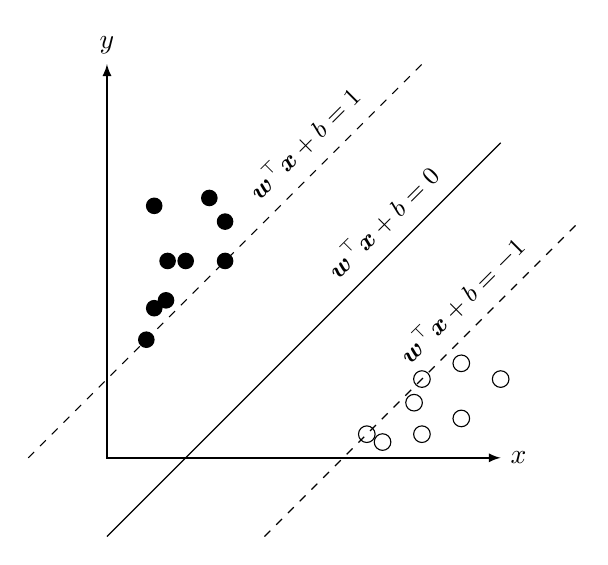
\begin{tikzpicture}
  % Draw axes
  \draw [doublearr] (0,5) node (yaxis) [above] {$y$}
        |- (5,0) node (xaxis) [right] {$x$};
  % draw line
  \draw (0,-1) -- (5,4); % y=x-1
  \draw[dashed] (-1,0) -- (4,5); % y=x+1
  \draw[dashed] (2,-1) -- (6,3); % y=x-3
  % \draw labels
  \draw (3.5,3) node[rotate=45,font=\small] 
        {$\vec{w}^\top \vec{x} + b = 0$};
  \draw (2.5,4) node[rotate=45,font=\small] 
        {$\vec{w}^\top \vec{x} + b = 1$};
  \draw (4.5,2) node[rotate=45,font=\small] 
        {$\vec{w}^\top \vec{x} + b = -1$};

  \fill[black] (0.5,1.5) circle (3pt);
  \fill[black]   (1.5,2.5)   circle (3pt);
  \fill[black] (1,2.5)     circle (3pt);
  \fill[black] (0.75,2)    circle (3pt);
  \fill[black] (0.6,1.9)   circle (3pt);
  \fill[black] (0.77, 2.5) circle (3pt);
  \fill[black] (1.5,3)     circle (3pt);
  \fill[black] (1.3,3.3)   circle (3pt);
  \fill[black] (0.6,3.2)   circle (3pt);
  % draw positive dots
  \draw[black] (4,1)     circle (3pt); 
  \draw[black] (3.3,.3)  circle (3pt); 
  \draw[black]     (4.5,1.2) circle (3pt); 
  \draw[black]     (4.5,.5)  circle (3pt); 
  \draw[black]     (3.9,.7)  circle (3pt); 
  \draw[black]     (5,1)     circle (3pt); 
  \draw[black]     (3.5,.2)  circle (3pt); 
  \draw[black]     (4,.3)    circle (3pt); 
\end{tikzpicture}
\caption{Diagram showing training points belonging to different classes (hollow versus solid dots) separated by a hyperplane $\vec{w}^\top \vec{x} + b = \pm 1$. The \LaTeX $\,$ script for this graph was originally created by Peng Yifan.}
\label{bg:svm:diag}
\end{figure}

The hyperplane is parameterised with weight vector $\boldsymbol w$ and bias $b$. We thus solve the classification problem using:
\begin{align}
f(\vec{x}) = \vec{w}^\top \vec{x} + b \label{bg:svm:linear_model}
\end{align}

Finding the hyperplane with maximum margin amounts to solving the following optimisation problem:
\begin{align}
\min_{w, b} \quad &\frac{1}{2} \boldsymbol w^\top \boldsymbol w \label{bg:svm:eq} \\
\text{subject to} \quad & y_i(\boldsymbol w^\top \boldsymbol x_i + b) \geq 1 \label{bg:svm:cond} 
\end{align}
for $i = 1, \dots , n$, where $y_i = \pm 1$, depending on the classification of the vector of features $\boldsymbol x_i$. Equation \ref{bg:svm:cond} is equivalent to:
\begin{gather*}
\boldsymbol w^\top \boldsymbol x_i + b \geq 1 \quad \text{if $y_i = 1$} \\
\boldsymbol w^\top \boldsymbol x_i + b \leq -1 \quad \text{if $y_i = -1$}
\end{gather*}


\subsection{Dual representation}
To solve the primal optimisation problem in (\ref{bg:svm:eq}) subject to the conditions in (\ref{bg:svm:cond}), we can formulate the following Lagrangian equation:
\begin{align}
L(\boldsymbol w, b, \boldsymbol a)
= \frac{1}{2} \boldsymbol w^\top \boldsymbol w - \sum_{i=1}^n a_i (y_i(\boldsymbol w^\top \boldsymbol x_i + b) - 1) \label{bg:svm:primal:eqn}
\end{align}
where $\boldsymbol a$ is the $n$-dimensional vector containing the Lagrangian multipliers ($a_i \geq 0$) corresponding to the inequality conditions in (\ref{bg:svm:cond}). The primal optimisation problem in (\ref{bg:svm:primal:eqn}) can be written as:
\begin{align}
\min_{\boldsymbol w, b} \max_{\boldsymbol a \geq 0} L(\boldsymbol w, b, \vec a) \label{bg:svm:primal}
\end{align}

This can be written as its dual equivalent:
\begin{align}
\max_{\vec a \geq 0} \min_{\vec w, b} L(\vec w, b, \vec a) \label{bg:svm:dual}
\end{align}

It can be shown that:
\begin{itemize}
\item The equation $L$ in (\ref{bg:svm:primal:eqn}) is convex, and thus any optimal solution found is guaranteed to be the global optimal solution \cite{RefWorks:123}.
\item The primal (\ref{bg:svm:primal}) and dual (\ref{bg:svm:dual}) problems have the same optimal solutions, if any \cite{RefWorks:124}.
\end{itemize}

To solve the problem in (\ref{bg:svm:dual}), we first minimise $L$ with respect to $\vec w$ and $b$ for fixed $\vec a$. To do this, we can take the derivative of $L$ with respect to $\vec w$ and $b$. Then, set the derivatives to 0.

\begin{align}
\frac{\partial L}{\partial b} &= - \sum_{i=1}^n a_i \, y_i \overset{!}{=} 0 \nonumber \\
\frac{\partial L}{\partial \vec{w}} &= \vec{w} - \sum_{i=1}^n a_i \, y_i \, \vec{x_i} \overset{!}{=} 0 \label{bg:svm:primal:partial}
\end{align}

This results in the constraints $a_i \geq 0$ and $\sum_{i=1}^n a_i \, y_i = 0$. Applying the above on equation \ref{bg:svm:primal:eqn}, we have:
\begin{align*}
L(\vec{a}) &= \frac{1}{2} \vec{w}^\top \vec{w} - \sum_{i=1}^n \left( a_i \, y_i \vec{w}^\top \vec{x_i} + a_i\,y_i \, b - a_i \right) \\
&= \frac{1}{2} \vec{w}^\top \vec{w} - \vec{w}^\top \underbrace{\sum_{i=1}^n  a_i \, y_i \, \vec{x_i}}_{=\vec{w}} - \, b \underbrace{ \sum_{i=1}^n a_i\,y_i}_{=0} + \sum_{i=1}^n a_i \\
&= \sum_{i=1}^n a_i - \frac{1}{2} \vec{w}^\top \vec{w}
\end{align*}

We would then obtain an expression of $L$ with respect to $\vec a$ that we maximise:
\begin{align*}
L(\vec a) = \sum_{i=1}^n a_i - \frac{1}{2} \sum_{i=1}^n \sum_{j=1}^n a_i a_j y_i y_j \vec{x}_i^\top \vec{x}_j
\end{align*}

Combining the above together with the constraints $a_i \geq 0$ and $\sum_{i=1}^n a_i y_i = 0$, we would get the following quadratic optimisation problem:
\begin{align*}
\max_{\vec a} \quad &\vec{1}^\top \vec a - \frac{1}{2} \vec{a}^\top \vec{K}_y \vec{a} \\
\text{subject to} \quad &a_i \geq 0, \quad i = 1, \dots , n \\
&\vec{a}^\top \vec y = 0
\end{align*}
where $\vec{1}$ is an $n$ dimensional vector of ones, and $\vec{K}_y = \left[ y_i \, y_j \, \vec{x}_i^\top \vec{x}_j \right]$.

From equation \ref{bg:svm:primal:partial},
\begin{align*}
\vec{w} = \sum_{i=1}^n a_i y_i \vec{x}_i
\end{align*}

Substituting this into the linear model equation in (\ref{bg:svm:linear_model}), we get:
\begin{align}
f(\vec{x}) = \sum_{i=1}^n a_i y_i \vec{x}_i^\top \vec{x} + b \label{bg:svm:decision}
\end{align}

In order to determine the classification of a new  point $\vec{x}$, we simply have to determine the sign of $f(\vec{x})$ in (\ref{bg:svm:decision}).

\subsection{Mapping to higher dimensional space}
When the relationship between data points in the input space is not linear, the linear SVM above would not be able to learn these non-linear relations. This would result in underfitting.

As such, we would need to map the input data points into a higher dimensional feature space. We can then build an SVM based on this higher dimensional space such that the points in this feature space is linearly separable.

We first define a mapping $\phi : X \rightarrow F$ where $\phi$ is a non-linear mapping from the input space $X$ to a higher dimensional feature space $F$. We then define the \textit{kernel} function $K$ such that $\forall \vec x, \vec y \in X$,
\begin{align*}
K(\vec x, \vec y) = \phi(\vec x)^\top \phi(\vec{y})
\end{align*}

The optimisation problem can then be written as:
\begin{align*}
\min_{\vec a} \quad &\frac{1}{2} \vec{a}^\top \vec{K}_y \vec{a} - \vec{1}^\top \vec a \\
\text{subject to} \quad &a_i \geq 0, \quad i = 1, \dots , n \\
&\vec{a}^\top \vec y = 0
\end{align*}
where $\vec{K}_y = y_i \, y_j \, \phi(\vec{x}_i)^\top \phi(\vec{x}_j) = y_i \, y_j \, K(\vec{x}_i, \vec{x}_j)$. Similarly, equation \ref{bg:svm:decision}, which determines the classification of a new data vector $\vec{x}$, can be written as:
\begin{align*}
f(\vec{x}) = \sum_{i=1}^n a_i y_i K(\vec{x}_i, \vec{x}) + b = \sum_{i=1}^n a_i y_i \, \phi(\vec{x}_i)^\top \phi(\vec{x}) + b
\end{align*}

Similarly to the linear case, we simply need to test the sign of $f(\vec{x})$ for a new vector $\vec{x}$. If $f(\vec{x})$ is positive, then we can classify it as class 1, and if $f(\vec{x})$ is negative we can classify it as class 2.

\subsection{Slack variables}
Our data may not be perfectly linearly separable in the feature space $\phi(\vec{x})$, especially due to the presence of noise \cite{RefWorks:127}. Slack variables, $\xi$, are introduced to allow some form of error when training data points are misclassified. These slack variables allow data points to be classified on the wrong side of the decision hyperplane, but the further away a point is from the decision boundary, the larger the penalty imposed. We then need one slack variable per input data point \cite{RefWorks:126}, defined as such:
\begin{itemize}
\item $\xi_i = 0$: data point is correctly classified.
\item $0 < \xi_i \leq 1$: data point lies inside the hyperplane margin, but is on the correct side of the boundary.
\item $\xi_i > 1$: data point is wrongly classified.
\end{itemize}

This is referred to as the \textit{1-norm soft margin} constraint in the literature \cite{RefWorks:127}. Now, we would need to maximise the margin of the hyperplane, while penalising the misclassified points. We can thus formulate our problem as such:
\begin{gather}
\min_{\vec{w}, b, \vec{\xi}} \quad \frac{1}{2}\vec{w}^\top \vec{w} + C \sum_{i=1}^n \xi_i \label{bg:svm:slack:primal} \\
\text{subject to} \quad y_i(\vec{w}^\top \vec{x}_i + b) \geq 1 - \xi_i , \quad 
\xi_i \geq 0 \quad \text{for $i = 1, \dots , n$}\label{bg:svm:slack:constraint}
\end{gather}
where $C>0$ is the \textit{penalty parameter}. Similarly, to state the dual of (\ref{bg:svm:slack:primal}) subject to the conditions in (\ref{bg:svm:slack:constraint}), we need to compute the Lagrangian:
\begin{align*}
L(\vec{w}, b, \xi_i, a_i, r_i) =
\frac{1}{2} \vec{w}^\top \vec{w} + C \sum_{i=1}^n \xi_i - \sum_{i=1}^n a_i(y_i(\vec{w}^\top \vec{x}_i + b) - 1 + \xi_i) - \sum_{i=1}^n r_i\xi_i
\end{align*}
where $a_i \geq 0$ and $r_i \geq 0$ are the Lagrangian multipliers.

Similarly, we compute the derivatives of the above with respect to $\vec{w}$, $b$ and $\xi_i$ to get the following dual problem:
\begin{gather}
\min_{\vec{a}} \quad L(\vec{a}) = \frac{1}{2}\vec{a}^\top \vec{K}_y \vec{a} - \vec{a}^\top \vec{1} \label{bg:svm:quadprob1} \\
\text{subject to} \quad \vec{a}^\top \vec{y} = 0, \quad 0 \leq a_i \leq C \label{bg:svm:quadprob2}
\end{gather}
where $K_y = [y_i \, y_j \, \vec{x}_i^\top \vec{x}_j]$ and $C$ is the penalty parameter.

%Now, suppose we choose to map the input space into a higher dimensional feature space, we simply modify $K_y$ in the above problem:
%\begin{align*}
%K_y = [y_i \, y_j \, \phi(\vec{x}_i)^\top \phi(\vec{x}_j)]
%\end{align*}

We then need to solve the quadratic optimisation problem in (\ref{bg:svm:quadprob1}) subject to (\ref{bg:svm:quadprob2}).

\subsection{Model selection} \label{bg:ml:svm:model}
There are 4 widely used kernels:
\begin{itemize}
\item Linear kernel: $K(\vec{x}_i, \vec{x}_j) = \vec{x}_i^\top \vec{x}_j$
\item Polynomial kernel: $K(\vec{x}_i, \vec{x}_j) = (\gamma \, \vec{x}_i^\top \vec{x}_j + r)^d$
\item Radial basis function (RBF): $K(\vec{x}_i, \vec{x}_j) = \exp(-\gamma \, \| \vec{x}_i - \vec{x}_j \|^2)$
\item Hyperbolic tangent kernel: $K(\vec{x}_i, \vec{x}_j) = \tanh(\gamma \, \vec{x}_i^\top \vec{x}_j + r)$
\end{itemize}
where $r$, $d$, $\gamma>0$ are kernel parameters.

First, we would pick a kernel before the training process. Then, using a procedure such as $k$-fold cross validation, we would then find the most optimal kernel and penalty parameters ($C$). For example, if we choose the RBF kernel, we would  perform cross validation to obtain the most optimal parameters $\gamma$ and $C$.

A study in \cite{RefWorks:128} noted that the RBF kernel has less numerical difficulties than the polynomial kernel. We note that, $\forall \vec{x}_i, \vec{x}_j \in X$, for an RBF kernel,
\begin{align*}
\| \vec{x}_i - \vec{x}_j \|^2 \geq 0 \quad \text{and} \quad \gamma > 0 \quad \Rightarrow \quad 0 < K(\vec{x}_i, \vec{x}_j) \leq 1 
\end{align*}

On the other hand, for large $d$, the polynomial kernel might go to infinity or close to 0. Furthermore, the hyperbolic tangent kernel is not valid under certain kernel parameters \cite{RefWorks:254}.

Although the RBF kernel is more commonly chosen than the rest of the kernels listed above, \cite{RefWorks:128} also revealed that if the number of features is large, using the linear kernel may suffice, as the non-linear mapping provided by the RBF kernel may not necessarily improve performance. Furthermore, using the linear kernel would mean that we only need to investigate the optimal $C$ penalty parameter value.

Nevertheless, the conclusion made in \cite{RefWorks:128} might be data-dependent and ideally, we should determine empirically which kernel suits our data the best.

\subsection{Implementing classification with SVM}
Chang and Lin \cite{libsvm} developed \texttt{libsvm}, a library for SVMs, which allows the quadratic optimisation problem in (\ref{bg:svm:quadprob1}) to be solved analytically \cite{RefWorks:126}. Furthermore, the library can be interfaced to other programming languages like Java, MATLAB and Python.

The Python library \texttt{scikit-learn} also allows SVMs to be trained for classification purposes (\texttt{SVC}) and allows various kernels to be used. \texttt{scikit-learn} also uses \texttt{libsvm} internally to handle computations.

\section{Feature selection} \label{bg:feature_selection}

This section explores the literature of feature selection, and discusses some algorithms and methodologies employed in the literature. The following terms will be used throughout this paper:
\begin{itemize}
  \item $D$: Original data set.
  \item $M$: Number of features in $D$. That is, $|D| = M$.
  \item $S$: Reduced subset of features selected by feature selection algorithm.
  \item $k$: Number of features in $S$, where $k \ll M$. That is, $|S| = k$.
\end{itemize}

\subsection{Purpose and motivation} \label{bg:fs:purpose}
% Overview of purpose of FS.

Discriminant analysis is key to this project. In the context of data with high dimensions, one of the main concerns of discriminant analysis is feature selection: instead of using all of the features to predict the result of the classification, we want to use only a small subset of the features. This subset should be representative of all the features.

We can also visualise the data set as a matrix, with columns as features and rows as samples. Then, the feature selection problem is akin to finding a smaller matrix with fewer columns that can be used more efficiently than the original matrix \cite{RefWorks:163}.

The process of feature selection can be described as finding a subset $S$ of the original $M$ features, such that the cardinality of $S$ is $k$, where $k \ll M$. It is essential that classification accuracy using these $k$ features should not be significantly lower than using all $M$ features. Finding $S$ that satisfies these criteria is the main concern of feature selection.

As mentioned in section \ref{intro_ML}, the data suffers from the curse of dimensionality, where the number of features is much higher than the number of samples. This usually causes over-fitting \cite{RefWorks:115, RefWorks:175}. This refers to the situation where the classifier can classify the training data perfectly, but performs poorly with unseen data \cite{RefWorks:98}. This is a common challenge in classification, and reducing the dimensions of the original data set often helps reduce overfitting \cite{RefWorks:228}. As such, feature selection will play an important preprocessing role in allowing us to understand the data better.

Overall, there are several benefits associated with feature selection that are often mentioned in literature \cite{RefWorks:140}:
\begin{itemize}
  \item \textbf{Savings in computational cost.} Reducing the number of features by removing what Kudo and Sklansky call \textit{garbage features} \cite{RefWorks:210} can improve the computational cost of our algorithm. This includes the cost incurred for training a classifier, and using the classifier to perform predictions.
  \item \textbf{Interpretable results.} In contrast to feature extraction, feature selection retains the properties of the original features. For this project, ideally, we want to be able to obtain a compact subset of features from which we can draw biological conclusions. This will be discussed in more detail in section \ref{bg:fs:extraction}.
  \item \textbf{Improvement in classification accuracy.} Due to experimental faults or the nature of the data, more features might lead to more noise in our data set \cite{RefWorks:163, RefWorks:197}. Having a more compact subset to train our classifier might improve the performance of the classifier \cite{RefWorks:174}. Furthermore, if selected well, a compact subset of features can generalise better than when all features are used \cite{RefWorks:233}.
\end{itemize}

\subsection{Feature selection versus feature extraction} \label{bg:fs:extraction}

In contrast to feature selection, feature extraction techniques, such as principal component analysis (PCA) and Linear Discriminant Analysis (LDA), result in a set of features that is a \textit{transformation} or combination of the original features. In other words, the original features are transformed into a space with lower dimensions. For example, PCA employs a transformation to map features to a space spanned by its principal components.

Feature extraction reduces the dimensions of the data by generating a set of new features. This implies that the interpretation of the original features is lost through the transformation. Furthermore, the original features in the data might contain features that are redundant or irrelevant to the target class (see section \ref{bg:fs:relevance}). Such features should ideally be removed.

In contrast, feature selection methods preserve the original features by simply removing those that are not relevant to the classification task. In general, feature extraction is performed when model accuracy is more important than model interpretability \cite{RefWorks:163}. However, in this project, we would want to obtain features that are biologically relevant, and can be interpreted by an expert \cite{RefWorks:192}. This allows us to extract biological conclusions from the reduced set of features \cite{RefWorks:142}.

Due to these reasons, this project will focus on feature selection instead of feature extraction.

\subsection{Classification of feature selection methods} \label{bg:fs:classification}

Feature selection methods can be categorised into one of the following \cite{RefWorks:117, RefWorks:118}:

\begin{itemize}
\item \textbf{Filters} rank features with either a univariate or multivariate measure. The former evaluates each feature individually, and selects only the top ranking features, while the latter evaluates subsets of features. No learning is involved in filters; they are independent of the classifier \cite{RefWorks:216}. In general, filters consider how each feature contributes to the classification of the targets, although interaction between features is not considered \cite{RefWorks:232}. Filter methods include $t$-test, information gain, $F$-test and the $\chi^2$-statistic.

\item \textbf{Wrappers} regard the learning algorithm as a black box \cite{RefWorks:140}, and evaluate features based on the classification accuracy of the learner. Wrappers usually incur more computational cost from training the classifier and using it for prediction.

\item \textbf{Embedded} methods incorporate the feature selection process into the training of the classifier. These methods combine the search in the feature space and the space of learning hypotheses, but they are specific to the choice of the classifier \cite{RefWorks:118}.

\item \textbf{Hybrid} methods are usually a combination of the above approaches. For example, a method can use a filter-like approach to individually rank features, and then use a classifier to evaluate subsets of features \cite{RefWorks:140}.

\end{itemize}

\subsection{Feature selection methods and trade-offs} \label{bg:fs:tradeoff}

The categories described above have their own merits and drawbacks. For example, as filters are independent of the classifier, they usually incur less computational cost. Furthermore, scoring each feature is usually independent of the other features, which means that the filter process can be parallelised. However, most filters are univariate, and thus do not consider feature redundancy or feature interaction. One can use multivariate filters which consider subsets of features, but these incur more computational cost.

On the other hand, wrappers are reported to produce better classification accuracy than filters \cite{RefWorks:163}, since they directly use a classifier to select features. At the same time, this means that wrappers are closely associated with the choice of learning algorithm, and might not generalise to other classifiers. One can also consider employing a ``two-stage'' process, such as in \cite{RefWorks:216}, where a filter is first used to remove unimportant features, and a classifier-dependent method can then be used to further refine the remaining features. Yet, one also needs to consider the number of features the first filter step should remove.

Indeed, Bolón-Canedo \textit{et. al} \cite{RefWorks:163} and Sharma \textit{et. al} \cite{RefWorks:215} echo these trade-offs, by pointing out that ``the best method'' does not exist and that no single algorithm stands out in all aspects. Furthermore, Hua \textit{et. al} \cite{RefWorks:216} performed a review of feature selection algorithms using different data sets, and concluded that none of the methods that were reviewed performed consistently well across all the data sets. This sentiment is also reflected in \cite{RefWorks:217}.

To this end, previous works on feature selection seek to find a method that reports good classification accuracy for a \textit{specific problem setting}. When one proposes a novel method or modification of a feature selection algorithm, one would compare the accuracy scores with other existing algorithms in the literature, and determine if their proposed method has an improvement over existing ones for a particular problem. We adopt this strategy in this project.

\subsection{Terminating feature selection algorithms} \label{bg:fs:terminating}

Feature selection algorithms can be terminated via the following ways \cite{RefWorks:210}:
\begin{itemize}
  \item \textbf{Specifying $k$}: The algorithm stops when the desired number of features in $S$ is obtained.
  \item \textbf{Satisfactory performance}: The algorithm terminates when the performance of $S$ exceeds a specified threshold. For example, we can quantify this performance using cross validation scores of a classifier.
  \item \textbf{No significant improvement}: The algorithm can terminate when the performance of $S$ does not improve much \cite{RefWorks:215}.
  \item \textbf{Balance between performance and subset size}: Optimise both classifier performance and $k$ simultaneously by maximising performance and minimising $k$.
\end{itemize}

From most works in feature selection, authors often specify a fixed value of $k$. In \cite{RefWorks:119} by Tang \textit{et. al}, the authors initially set $k=100$ for all the datasets that were used, but later recommended different values of $k$ for two of these datasets. This suggests that $k$ is dependent on the dataset.

If $k$ is not a constraint of the problem, we could perform a grid search to find an optimal $k$. However, due to time and computational constraints, one will probably not be able to perform a grid search on all possible values of $k$ (i.e. $k \in [1, M]$), but only on an interval $\theta \subset [1, M]$. So, even if we find an optimal $k$ in $\theta$, it is most likely only a local optimum.


\subsection{Exhaustive versus heuristic search} \label{bg:fs:exhaustive}

One obvious but naive way to find $S$ would be to exhaustively consider all possible subsets of the original feature space, and select the one that gives the best classification performance.

With $M$ features, an exhaustive search would iterate through $2^M$ subsets \cite{RefWorks:182}. Intuitively, for each feature in $M$, it can either be inside the selected subset, or not. We can prove this formally via induction.

\begin{proof}
The exhaustive search would require us to search through the space of all subsets, where for each subset $S$, $|S| \in \left[ 0, M \right]$. We include the trivial cases of $|S|=0$ (all $M$ features do not contribute to the classification) and $|S|=M$ (all $M$ features are important). Then, we want to prove that the number of subsets searched is $2^M$:
\begin{align*}
\text{No. } &\text{of subsets with 0 feature} + \text{No. of subsets with 1 feature} \\ & + \dots + \text{No. of subsets with $M$ features} \\
&= {{M}\choose{0}} + {{M}\choose{1}} + \dots + {{M}\choose{M}} \\
&= 2^M
\end{align*}

where, ${{M}\choose{k}} = \frac{M!}{k!(M-k)!}$ is the number of subsets with cardinality $k$. 

For $M=1$, the total number of subsets searched is:
\begin{align*}
{{1}\choose{0}} + {{1}\choose{1}} = 2^1
\end{align*}

Suppose $M=k$ is true, for an arbitrary $k>1$. Then, the number of subsets searched would be
\begin{align*}
{{k}\choose{0}} + {{k}\choose{1}} + {{k}\choose{2}} + \dots + {{k}\choose{k}} = 2^k 
\end{align*}

For $M=k+1$, the total number of subsets searched is:
\begin{align}
&{{k+1}\choose{0}} + {{k+1}\choose{1}} + {{k+1}\choose{2}} + \dots + {{k+1}\choose{k}} + {{k+1}\choose{k+1}} \nonumber \\
&= {{k}\choose{0}} + \left[ {{k}\choose{0}} + {{k}\choose{1}} \right] + \left[ {{k}\choose{1}} + {{k}\choose{2}} \right] + \dots + \left[ {{k}\choose{k-1}} + {{k}\choose{k}} \right] + {{k}\choose{k}} \label{exhaustive:second} \\
&= 2 \left[ {{k}\choose{0}} + {{k}\choose{1}} + \dots + {{k}\choose{k}} \right] \nonumber \\
&= 2 \left(2^k \right) \nonumber \\
&= 2^{k+1} \nonumber
\end{align}
where in (\ref{exhaustive:second}), the following results were used:
\begin{gather*}
{{n}\choose{k}} = {{n-1}\choose{k-1}} + {{n-1}\choose{k}} \\[1em]
{{k+1}\choose{0}} = {{k}\choose{0}} = 1 \quad \text{and} \quad {{k+1}\choose{k+1}} = {{k}\choose{k}} = 1
\end{gather*}
So, for any $M\geq 1$, the number of subsets searched by an exhaustive search is $2^M$.
\end{proof}

Evidently, although an exhaustive search would guarantee an optimal subset, its runtime complexity would be prohibitively high. As Sima and Dougherty put it, \textit{``A major impediment to feature selection is the combinatorial nature of the problem''} \cite{RefWorks:191}. Thus, most of the algorithms in the literature of feature selection trade the optimality guaranteed in exhaustive search for lower computational cost. These methods involve heuristics to guide the search for $S$. Some examples would be discussed in the following sections.

\subsection{Feature relevance and feature redundancy} \label{bg:fs:relevance}

Relevance and redundancy play important roles in the literature of feature selection. In \cite{RefWorks:163}, Bolón-Canedo \textit{et. al} assert that ``\textit{detecting the relevant features and discarding the irrelevant and redundant ones}'' are processes that define feature selection.

In general, a feature is \textit{relevant} if it is closely related to the target class; in other words, it has a large influence on the outcome of the classification of the samples. For example, one can evaluate the relevance of each feature through some measure such as the $t$-statistic and rank the relevance of the features. It is tempting to select the first $k$ features as our subset $S$, but as Peng \textit{et. al} put it, ``\textit{The best $k$ features are not the $k$ best features}'' \cite{RefWorks:182}, as the highly ranked features are likely to have similar discriminating power \cite{RefWorks:163}. In other words, some features among these $k$ features might be redundant.

A feature $f_1$ is \textit{redundant} with respect to another feature $f_2$, if $f_1$ is ``similar'' to $f_2$. This similarity can be quantified in many ways and mutual information is often used (see section \ref{bg:fs:mi}). \cite{RefWorks:187} describes the ``ultimate feature redundancy'' as two features having exact linear dependency. For example, $f_1$ and $f_2$ might be linked by the equation $f_1 = 2 \, f_2$, and thus $f_2$ does not provide additional information in the presence of $f_1$ (or vice versa).

%Greedy searches, which will be explained in detail in the later sections, use relevance and redundancy to guide the search in the feature space. For example, it evaluates a subset of features based on, say, classification score of a machine learner, to determine the discriminating power of that subset.

In the context of this project, there is a possibility that not all of the features in our data set have a role to play in the classification of schizophrenia. As such, quantifying relevance and redundancy is necessary to select the significant features and eliminate the others. Besides, once we obtain a compact subset $S$, it would be computationally cheaper to train our classifier based on just these features.


\subsection{Greedy search} \label{bg:fs:greedy}
As mentioned in section \ref{bg:fs:purpose}, the cost of an exhaustive search on all possible subsets of all $M$ features is exponential with $M$. Even though the exhaustive search guarantees an optimal solution, its computational cost does not scale with more features. As a result, many algorithms involve heuristics to guide the search for the optimal subset $S$. Although none of the methods which use heuristics can guarantee an optimal solution, these methods improve the computational cost of finding $S$, which is very beneficial in the context of high dimensional data, making these methods more practical to execute \cite{RefWorks:140, RefWorks:182}. These methods are thus classified as sub-optimal.

For example, the \textit{sequential forward selection} (SFS) \cite{RefWorks:177} is a wrapper method that involves a greedy search strategy. The method starts with $S=\emptyset$. For each feature $m$, we compute an evaluation function, $J(\cdot)$. In this context, $J(\cdot)$ is the classification score of the learner from just using 1 feature. The scores are then sorted, and the feature with the highest score (call it $f_1$) is selected. That is, if $F$ represents the set of all features, then:
\begin{align*}
\forall f_k \in F, \quad J(f_1) \geq J(f_k)
\end{align*}

 $f_1$ is then paired sequentially with each of the remaining features to form a subset, and classification scores using just 2 features are obtained and sorted. That is, we obtain classification scores for the sets
\begin{align*}
\left\lbrace f_1, f_2 \right\rbrace, \left\lbrace f_1, f_3 \right\rbrace, \dots, \left\lbrace f_1, f_M \right\rbrace
\end{align*}
  
Let $f_2$ be the feature where the set $S= \left\lbrace f_1, f_2 \right\rbrace$ has the highest classification score. We now pair another of the remaining features with $S$ and find classification scores. This process continues until we have our desired $k$ features.
  
A variant is the \textit{sequential backward selection} (SBS), which starts with all $M$ features instead. SBS sequentially removes one feature. That is, SBS starts with the full set of $M$ features and works backwards. This means that SBS will take a longer time than SFS to give us our desired number of features $k$, especially when $k$ is a small number \cite{RefWorks:190}, since we will need to iterate through each feature and fit a classifier using a large number of features. It is suggested that SBS might give us a better result, but we will end up with larger feature subsets and longer computational time \cite{RefWorks:208}.

Another variant is the \textit{floating forward/backward search} strategy proposed by Pudil \cite{RefWorks:178}. Pudil noted that both SFS and SBS suffered from a ``nesting effect'', where previously selected or discarded features cannot be considered again in SFS and SBS respectively. The floating variant tackles this problem.

Lastly, Deng \cite{deng1998omega} proposed the \textit{Restricted Forward Selection} (RFS), which is an even greedier variant of SFS. Suppose we have a sorted list of the classification scores when each feature is considered singly. That is,
\begin{align*}
J(f_1) > J(f_2) > \dots > J(f_M)
\end{align*}
%Suppose the corresponding features are $S =\left\lbrace f_1, f_2, \dots , f_M \right\rbrace$. That is,

$f_1$ would be selected as the first feature. While SFS considers all of the remaining features, RFS only considers those features that perform well individually. We thus consider the pairs $\left\lbrace f_1, f_2 \right\rbrace, \left\lbrace f_1, f_3 \right\rbrace$ all the way to $\left\lbrace f_1, f_{M/2} \right\rbrace$, and select the best subset. That is, we only consider $M/2$ of the sorted features that perform best individually.

The fact that RFS considers only part of the sorted features makes it a greedy variant of SFS. The pseudocode of RFS is listed in algorithm \ref{RFSAlgo}. In algorithm \ref{RFSAlgo}, the list $L$ represents the sorted list of $(feature, score)$ pairs where $score$ is the cross validation (CV) score obtained by using 1 feature only.

\begin{algorithm}
\DontPrintSemicolon
\KwIn{Data set $D$ with $M$ features.}
\KwOut{Subset $S$ ($S \subset D$) of the $M$ features such that $|S|=k$, $k \ll M$.}
\BlankLine
\Begin{
Initialise empty list $L \longleftarrow [\,]$\;
Initialise empty list $S \longleftarrow [\,]$ \;
\For{$i=1 \longrightarrow M$}{
$s \longleftarrow$ CV score for $i$-th feature. \;
$L \longleftarrow L \cup \left\lbrace (i,s) \right\rbrace$ \;
}
$w \longleftarrow $ feature that corresponds to $\max s$ in $L$. \;
$S \longleftarrow S \cup \left\lbrace w \right\rbrace$ \;
\BlankLine
\For{$i=2 \longrightarrow k$}{
$num\_iterations \longleftarrow M / i$ \;
Initialise empty list $scores \longleftarrow [\,]$ \;
$j \longleftarrow 0$ \;
\While{$|scores| \leq num\_iterations$} {
\If{feature in $L[\,j\,] \in S$} {
$j \longleftarrow j + 1$ \;
\textbf{continue}
}
\BlankLine
$S_j \longleftarrow S \cup \left\lbrace \text{feature in } L[\,j\,] \right\rbrace$ \;
$s \longleftarrow $ CV score for $S_j$. \; 
$scores \longleftarrow scores \cup \left\lbrace (j,s) \right\rbrace$. \;
$j \longleftarrow j + 1$ \;
}
$w \longleftarrow $ feature that corresponds to $\max s$ in $scores$. \;
$S \longleftarrow S \cup \left\lbrace w \right\rbrace$
}
}
\caption{Restricted Forward Selection($D$, $k$) \label{RFSAlgo}}
\end{algorithm}


\subsection{Recursive feature elimination} \label{bg:fs:rfe}
Another flavour of search is the Recursive Feature Elimination (RFE), first proposed by Guyon \textit{et. al} in \cite{RefWorks:228} and it has been used in \cite{RefWorks:229, RefWorks:230, RefWorks:231}. In particular, Guyon \textit{et. al} focused on RFE when used with SVMs. RFE can thus be classified as a wrapper method.

From section \ref{bg:svm}, fitting an SVM with a linear kernel boils down to solving the problem:
\begin{align*}
L(\boldsymbol w, b, \boldsymbol a)
= \frac{1}{2} \boldsymbol w^\top \boldsymbol w - \sum_{i=1}^n a_i (y_i(\boldsymbol w^\top \boldsymbol x_i + b) - 1)
\end{align*}

where the weight vector $\vec{w}$ and bias term $b$ are parameters of the hyperplane that separates the data points:
\begin{align*}
f(\vec{x}) = \vec{w}^\top \vec{x} + b
\end{align*}

Furthermore, to determine the classification of an input vector $\vec{x}$, we can simply compute:
\begin{align*}
y(\vec{x}) = sign(\vec{w}^\top \vec{x} + b)
\end{align*}

Thus, evidently, the input vectors $\vec{x}$ that have the highest corresponding weights $\vec{w}$ will contribute the most to the classification of $\vec{x}$ \cite{RefWorks:229}. This motivates the RFE.

In RFE, a classifier is first trained using all of the features. The weight of each $i$-th feature, $w_i$, is then computed. RFE eliminates insignificant features by removing features with the lowest weights $\vec{w}$. This procedure is repeated until the desired number of features is obtained. In cases where features are eliminated one at a time, RFE can be viewed as a \textit{feature ranking} procedure, since we rank features according to their weights. Otherwise, it is considered a \textit{feature subset ranking} procedure.

Evidently, RFE is a greedy algorithm, as it progressively reduces the subset of features it considers, and does not consider features that have been eliminated. Thus, RFE considers \textit{nested} subsets of features.

Furthermore, as RFE iteratively removes features, it works similarly to the sequential backward selection (SBS) method. As such, one disadvantage of RFE is that it might be computationally inefficient, as the algorithm trains a classifier using all of the features at first, and progressively reduces the number of training features. However, Guyon \textit{et. al} suggested removing several features at a time, making RFE a feature subset ranking algorithm. Evidently, optimality will be compromised in this manner.


\subsection{Optimal search by branch-and-bound}
It is also worth mentioning the work of Narendra and Keinosuke \cite{RefWorks:176}, who proposed a branch-and-bound algorithm to demonstrate that an optimal solution can still be obtained without an exhaustive search. Even though the paper showed that substantial savings were made in terms of number of subsets evaluated, the algorithm does not scale to high-dimensional data \cite{RefWorks:178} due to its exponential time complexity \cite{RefWorks:190, RefWorks:189}. For example, the paper demonstrated the use of the branch-and-bound algorithm to choose only 12 features from 24. As such, we will not look into this method any further, as the other types of search, though less optimal, do not involve exponential time complexity.

\subsection{Use of mutual information in feature selection} \label{bg:fs:mi}

A common heuristic to quantify relevance and redundancy is mutual information (MI) \cite{RefWorks:98}. MI can be interpreted as a measure that quantifies the dependence between variables $X$ and $Y$ \cite{RefWorks:180} and the amount of information $X$ carries about $Y$ \cite{RefWorks:181}. 

For discrete random variables $X$ and $Y$, the MI between them, $I(X, Y)$, is given by:
\begin{align} \label{bg:fs:mi:dis}
I(X, Y) = \sum_{x \in X} \sum_{y \in Y} p(x, y) \log_2 \left(\frac{p(x, y)}{p(x) \, p(y)} \right) 
\end{align}

For continuous variables, the sum will simply change to an integral:
\begin{align} \label{bg:fs:mi:cont}
I(X, Y) = \int_{x \in X} \int_{y \in Y} p(x, y) \log_2 \left( \frac{p(x, y)}{p(x) \, p(y)} \right) dy \, dx
\end{align}

For a combination of discrete and continuous random variables, we would simply use the sum or integral respectively. For example, we can calculate the MI between a target class $C$ and a continuous feature $X$ by evaluating:
\begin{align*} %\label{bg:fs:mi:contDis}
I(X, C) = \int_{x \in X} \sum_{c \in C} p(x, c) \log_2 \left( \frac{p(x, c)}{p(x) \, p(c)} \right) dx
\end{align*}

An example of a feature selection algorithm that makes use of MI extensively is the \textit{minimal-redundancy maximal-relevance} (mRMR) algorithm \cite{RefWorks:182}. mRMR maximises relevance between a feature set $S$ and target class $c$ by maximising the MI between them. That is,
\begin{align*}
\max \, D(S, c) = \frac{1}{|S|} \sum_{x_i \in S} I(x_i, c)
\end{align*}

This heuristic maximises the discriminative power of each feature in $S$.

Furthermore, mRMR minimises redundancy between features in the feature set $S$ by minimising the MI between features in $S$. That is,
\begin{align*}
\min \, R(S) = \frac{1}{|S|^2} \sum_{x_i, x_j \in S} I(x_i, x_j)
\end{align*}

However, the main difficulty in using MI is the estimation of the joint and marginal probabilities ($p(x, y)$ and $p(x)$ or $p(y)$ respectively in equations \ref{bg:fs:mi:dis} and \ref{bg:fs:mi:cont}). For discrete or categorical variables, estimating the probabilities would simply be obtained from frequency counts \cite{RefWorks:183}, although the estimation would only be accurate if we have enough samples \cite{RefWorks:182}. Yet, with more classes and more states in each class, the estimation of the joint probability would become more difficult \cite{RefWorks:140}.

In the case of continuous variables, the computation of MI would be even harder \cite{RefWorks:185}, as we would need to compute the integral of the continuous probabilities \cite{RefWorks:192}. A way to avoid computing integrals is to discretise the continuous variables. We can estimate the probabilities of continuous variables by discretising the values into \textit{bins} (discrete intervals). A histogram can be created to investigate the distribution of the bins. However, we will have to determine an appropriate width for the intervals (or an appropriate number of bins), which will influence the estimates significantly \cite{RefWorks:186}. We should also note that the features in the data for this project are continuous. 

Another method to estimate these probabilities is by using the \textit{Parzen Window} method, as proposed by Kwak and Choi in \cite{RefWorks:183}. Although the work has shown that using the Parzen Window leads to better performances when combined with certain feature selection algorithms, one still has to specify certain parameters associated with the Parzen Window, such as the \textit{window function} and the \textit{window width}. These need to be correctly specified for the estimated probabilities to converge to the true probability \cite{RefWorks:184}. Kwak and Choi used the Gaussian window with a fixed window width. However, these choices were not explained sufficiently. They have also made certain assumptions about the covariance of the variables, but these assumptions might not hold for all types of data sets. Nevertheless, with sufficient time, one could perform a search to find an optimal window width using different window functions.

Consequently, methods such as \textit{maximum relevance minimum multicollinearity} (MRmMC) \cite{RefWorks:187} avoid the complexity of estimating MI involving continuous variables by proposing other measures to quantify relevance and redundancy. This will be discussed in section \ref{mrmmc}.

\section{Genetic algorithms in feature selection} \label{bg:fs:ga}

Genetic algorithms (GAs) are a type of heuristic search method that explores solutions by repeatedly evolving and combining them. It is based on the theory of evolution and its concept of \textit{natural selection} and \textit{survival of the fittest} \cite{RefWorks:205}. GAs search through a space of potential solutions by using probabilistic genetic operators to avoid local optima and produce better solutions \cite{RefWorks:210, RefWorks:207, RefWorks:211}. Although GAs are reported to take more time to select features, they can explore a wider variety of subset features \cite{RefWorks:232}.

The following terms are often used in the context of GAs:
\begin{itemize}
  \item A \textbf{chromosome} describes a solution \cite{RefWorks:205, RefWorks:209}. Usually, a chromosome uses a \textit{binary encoding} to represent a solution. An array, say $A$, can be used to store a chromosome. In the context of feature selection, each element in the array, $A[\,i\,]$, is either 0 or 1, which means the $i$-th feature is not selected or a feature is selected, respectively.
  
  \item The $i$-th \textbf{generation} describes the $i$-th iteration of the GA.
  
  \item A \textbf{population} is the set of chromosomes (solutions) in a generation.
\end{itemize}

The following terms are inspired by evolution, and characterise the probabilistic aspect of a GA:
\begin{itemize}
  \item \textbf{Fitness} quantifies how desirable a chromosome is with respect to the problem the GA is trying to solve. For example, \cite{RefWorks:204} uses classification error as its fitness criteria, \cite{RefWorks:200} uses both the classification error and the dimension of a chromosome, while \cite{RefWorks:201} uses correlation between two variables.
  
  \item Two parents can perform a \textbf{crossover} to produce a pair of potentially fitter offsprings. There are several strategies for the crossover operator, such as one-point \cite{RefWorks:201}, two-point \cite{RefWorks:202, RefWorks:204} and uniform crossover \cite{RefWorks:222}. These will be discussed in section \ref{bg:ga:crossover_sect}.
  
  \item The \textbf{mutation} operator probabilistically selects and changes one or more elements of a chromosome. For example, \cite{RefWorks:201, RefWorks:204} use a uniform distribution to select these elements. In the context of feature selection, the chosen element will have its bit inverted.

  \item The \textbf{selection} process selects parents for the crossover process. Depending on the strategy that one employs, the parents might simply be the two fittest chromosomes or they might be randomly selected. One can also choose chromosomes with the worst fitness for crossover, in hope that this will raise the overall fitness of the population \cite{RefWorks:203}.
  
%the selected chromosome(s) will either be selected as parents for crossover, or they will be retained and moved to the next generation (\textit{elitism/cloning}  strategy \cite{RefWorks:202, RefWorks:212, RefWorks:227}). One can also select the chromosomes with 
  
\end{itemize}

These operators are responsible for evolving a population and they help to increase the \textit{diversity} of a population, which can be interpreted as a balance between \textit{exploitation and exploration} \cite{RefWorks:236}: changing a good solution encourages the algorithm to explore other solutions, possibly allowing us to escape a local optimum.

GAs encapsulate the concept of \textit{survival of the fittest}, since the fitter a chromosome is, the more likely it is either copied to the next generation (\textit{elitism/cloning} \cite{RefWorks:202, RefWorks:212, RefWorks:227}), or selected as a parent for crossover \cite{RefWorks:209}. Furthermore, Kudo and Sklansky also recommend GAs for ``large-scale'' problems that involve more than 50 features \cite{RefWorks:210}. A typical genetic algorithm is illustrated in the flowchart in Figure \ref{bg:fs:ga:flowchart}.

Moreover, GAs do not require gradients to find an optimum solution. This avoids the numerical and computational complexity associated with other search methods \cite{RefWorks:242}. GAs can also take advantage of parallelism to speed up computation (see section \ref{body:parallel}).

As an extension proposed by the authors, we investigate if incorporating a GA with the MRmMC method will improve its performance. This will be discussed in detail in section \ref{ga:mrmmc}.

\begin{figure}
\centering
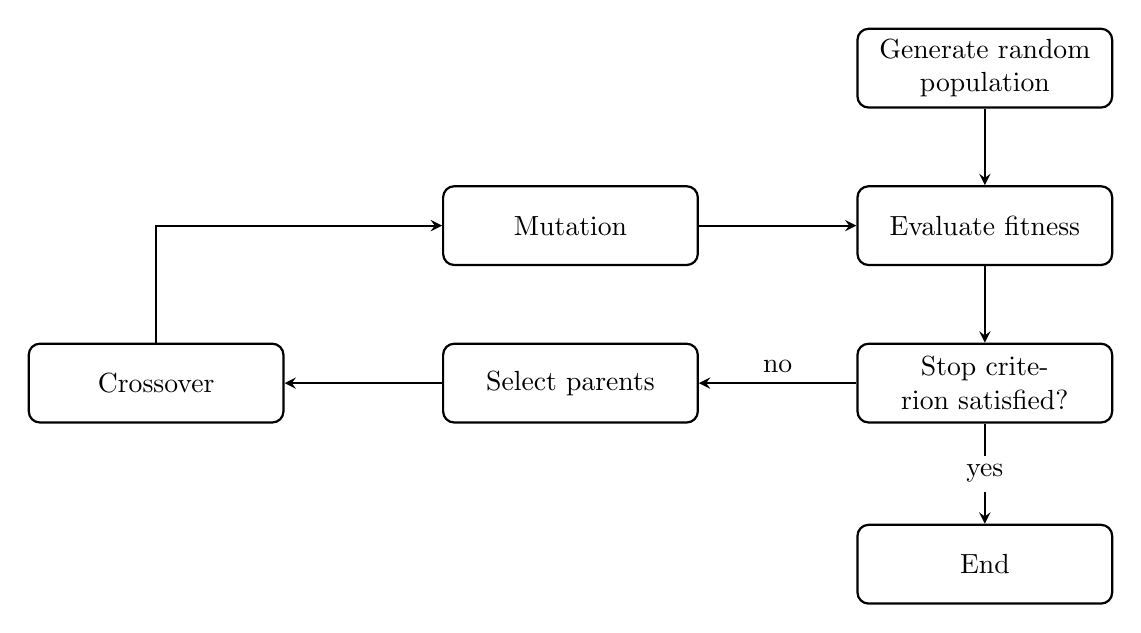
\begin{tikzpicture}[node distance=2cm]

  [ ->,
    >=stealth',
    shorten >=1pt,
    auto,
    node distance=2.5cm,
    thick
    ]

\node (start) [node] {Generate random population};
\node (fitness) [node, below of=start] {Evaluate fitness};
\node (stop) [node, below of=fitness] {Stop criterion satisfied?};
\node (end) [node, below of=stop, yshift=-0.3cm] {End};
\node (select) [node, left= of stop] {Select parents};
\node (cross) [node, left =of select] {Crossover};
\node (mutation) [node, above of=select] {Mutation};

\draw [arrow] (start) -- (fitness);
\draw [arrow] (fitness) -- (stop);
\draw [arrow] (stop.south) -- node[fill=white]{yes} (stop|-end.north);
\draw [arrow] (stop) -- node[anchor=south] {no}(select);
\draw [arrow] (select) -- (cross);
\draw [arrow] (cross.north) |- (mutation.west);
\draw [arrow] (mutation.east) to (fitness.west);

\end{tikzpicture}
\caption{Flowchart showing the steps that are usually involved in a typical genetic algorithm.}
\label{bg:fs:ga:flowchart}
\end{figure}

\subsection{The two-stage genetic algorithm}\label{bg:ga:twostage}
There are several ways to implement GAs, and each has its merits and drawbacks. For example, a method described by Mitchell in \cite{RefWorks:205} initially generates $p$ solutions at random. This method is used in \cite{RefWorks:206}, where 20 solutions are randomly generated to form the initial population of the GA and each solution will contain $M$ 0's and 1's where $M$ is the total number of features available. We note that the GA in \cite{RefWorks:206} was performed on a dataset of only 9 features. Thus, the array representing a solution will have 9 elements each. However, in the context of our project, storing 20 arrays of size over 400000 each might impose a large memory demand.

In contrast, several works such as \cite{RefWorks:197, RefWorks:198, RefWorks:199, RefWorks:200, RefWorks:203} utilise a GA in a ``two-stage'' process. First, a filtering step removes features that might be irrelevant to the target class or redundant with respect to other features. For example, \cite{RefWorks:197, RefWorks:198, RefWorks:203} use mutual information to conduct an initial filter on all the features. Second, the set of filtered features is then passed on to a GA to explore solutions in the reduced space. This idea is illustrated in Figure \ref{bg:fs:ga:twoStage}.

\begin{figure}
\centering
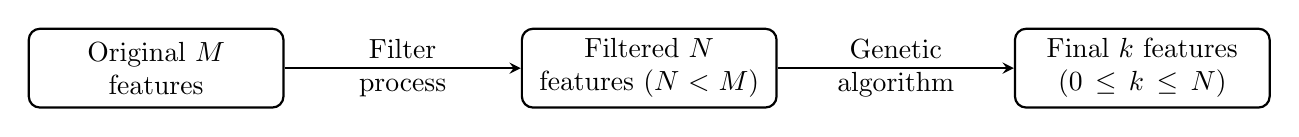
\begin{tikzpicture}[node distance=3cm]
\node (original) [node] {Original $M$ features};
\node (filtered) [node, right=of original] {Filtered $N$ features ($N<M$)};
\node (final) [node, right=of filtered] {Final $k$ features $(0 \leq k \leq N)$};

\draw [arrow] (original) -- node {Filter process} (filtered);
\draw [arrow] (filtered) -- node {Genetic algorithm} (final);

\end{tikzpicture}
\caption{Flowchart depicting the two-stage genetic algorithm.}
\label{bg:fs:ga:twoStage}
\end{figure}

This two-stage process offers an improvement in terms of memory demand, as the filter process shrinks the dimension of the solution space for the GA. Instead of storing all 400000 features, we only need to keep track of the binary strings encoded for the reduced search space. Although \cite{RefWorks:201} argues that the reduced search space still contains features that are the most promising, the GA implemented this way evidently suffers from a compromise in optimality.

\subsection{Parameters and strategies of GAs}
Even though previous works using GAs have reported positive experimental results, one difficulty of GAs is the number of parameters that need to be tuned \cite{RefWorks:210}, including population size, crossover rate, and mutation rate.

Moreover, different strategies can be used in certain parts of the GA. For example, in the selection process, the parents can either be the solutions with the worst fitness \cite{RefWorks:203}, or selected in proportion to their fitness (\textit{Roulette Wheel selection}) \cite{RefWorks:205, RefWorks:227}. The mutation rate, which often takes a small value, say $m$, can range from  1\% to 15\% \cite{RefWorks:206}.

%This means that $m$ percent of a chromosome will be randomly chosen, and these elements will have their bits inverted.

One would need to investigate what parameters and/or strategies would work best for the data set, and justify any parameters that seem arbitrary. This is the heart of one of the extensions listed in section \ref{further_work}.

\subsection{Regarding crossover} \label{bg:ga:crossover_sect}
The crossover operator is an important step in a GA, and is considered to be the ``driving force'' of the GA, as it allows the algorithm to explore more solutions over the search space \cite{RefWorks:223, RefWorks:226}. Two aspects of crossover can vary: its rate and its type, which include one-point, two-point and uniform crossovers.

In the \textit{one-point} crossover, a position (crossover point) along a chromosome is randomly chosen. The segments partitioned by this position are swapped between the two parents to produce two offsprings. In the \textit{two-point} crossover (see Figure \ref{bg:ga:crossover}), two positions are chosen and the segments in the parent chromosomes are swapped. In the \textit{uniform} crossover, each position is chosen uniformly and is thus a potential crossover point.

The partition can be represented as a \textit{crossover mask} \cite{RefWorks:205}. Figure \ref{bg:ga:crossover} shows how the two-point crossover works. The crossover mask is a binary string with two segments of 1's. For one of the offsprings, ``1'' might represent ``copy bit from parent A'' while ``0'' might represent ``copy bit from parent B''. The instructions will be inverted for the other offspring. On the other hand, for a uniform crossover, the crossover mask is generated randomly.

What the crossover and mutation operators do is to ensure that segments of information encoded in each chromosome (also referred to as \textit{schemata} \cite{RefWorks:224}), are sampled sufficiently. In \cite{RefWorks:224}, Picek and Golub discuss the performance of the aforementioned crossover operators. They found that GAs that do not use any crossover operators, or those that use one-point crossovers do not perform as well as those that use uniform or two-point crossovers. We note that the uniform and two-point crossover strategies disrupt segments of information in a chromosome more extensively than the one-point crossover. For example, in Figure \ref{bg:ga:crossover_a}, a schemata is represented by dots. The crossover operation might disrupt this segment, as shown in Figure \ref{bg:ga:crossover_b}.

%Suppose that there is a segment along the chromosome that improves the performance of the subset selected, or is crucial to good performance. For example, this segment resembles the global optimum. This is illustrated by dots in Figure \ref{bg:ga:crossover_a}. The crossover might thus disrupt this segment, as shown in Figure \ref{bg:ga:crossover_b}.

\begin{figure}
\centering

\usetikzlibrary{chains}
\makeatletter
\tikzset{
  on chain/.append code={
    \ifnum\c@pgf@counta=1\relax
      \tikzset{every first on chain/.try}%
    \fi
  },
  start chain/.append code={%
    \edef\pgf@marshal{\noexpand\tikzset{execute at end scope={\noexpand\xdef\noexpand\tikzpreviouschain{\tikz@lib@chain@name}}}}%
    \pgf@marshal
  }
}
\def\listset{\pgfqkeys{/List}}
\tikzset{
  no line/.style={font=\strut,text depth=+0pt,minimum width=+1.2em, inner xsep=+0pt},
  raw sort entry/.style={rectangle, thick, draw, font=\strut,text depth=+0pt,minimum width=+1.2em, inner xsep=+0pt},
  sort entry black/.style={raw sort entry, black, fill=white},
  sort entry blackgray/.style={raw sort entry, black, fill=gray!25},
  s1/.style={raw sort entry, fill=yellow!30},
  s2/.style={raw sort entry, fill=green!20},
  s3/.style={raw sort entry, fill=orange!25},
  g/.style={raw sort entry, fill=lightgray},
  h/.style={raw sort entry},
  no/.style={no line}
}
\listset{
  chain name/.initial=,
  do/.style={
    /utils/exec={\begin{scope}[start chain=\pgfkeysvalueof{/List/chain name}]},
    int/do/.list={#1},
    /utils/exec=\end{scope},
  },
  int/do/.code={%
    \pgfutil@ifnextchar[\tikz@List@int@@do{\tikz@List@int@@do[]}#1\pgf@stop
  }
}
\def\tikz@List@int@@do[#1]#2\pgf@stop{%
  \node[on chain={\pgfkeysvalueof{/List/chain name}},#1] {#2};
}

\begin{subfigure}[b]{\textwidth}
\centering
\begin{tikzpicture}[
  node distance=+1em and +0pt,
  outer xsep=+0pt,
  outer ysep=+0pt,
]
 \listset{chain name=r1,do={[g], [g], [g], [g]•, [g]•, [g]•, [g]•, [g]•, [g], [g], [g], [g], [g], [g], [g], [g], [g], [g], [g], [g]}}
 \tikzset{every first on chain/.style={below=of \tikzpreviouschain-begin}}
 \listset{chain name=btw, do={[no]1, [no]1, [no]1, [no]1,[no]1, [no]0, [no]0, [no]0, [no]0, [no]0, [no]0, [no]0, [no]0, [no]0, [no]0, [no]1, [no]1, [no]1, [no]1, [no]1}}
 \tikzset{every first on chain/.style={below=of \tikzpreviouschain-begin}}
 \listset{chain name=r2, do={[h], [h], [h], [h],[h], [h], [h], [h], [h], [h], [h], [h], [h], [h], [h], [h], [h], [h], [h], [h]}}

 \foreach \column in {5,15}{
   \ifnum\column=0
     \draw[dash pattern=on \pgflinewidth off \pgflinewidth] ([yshift=1em]r1-begin.north west) -- ([yshift=-1em]r2-begin.south west);
   \else\ifodd\column
       \draw[densely dotted] ([yshift=.75em]r1-\column.north east) -- ([yshift=-.75em]r2-\column.south east);
     \else
       \draw[dash pattern=on \pgflinewidth off \pgflinewidth] ([yshift=1em]r1-\column.north east) -- ([yshift=-1em]r2-\column.south east);
     \fi
   \fi}
\end{tikzpicture}
\caption{Before crossover operation. The array in the middle is the crossover mask, and the two arrays are the two parent chromosomes.}
\label{bg:ga:crossover_a}
\end{subfigure}\\[2em]

\begin{subfigure}[b]{\textwidth}
\centering
\begin{tikzpicture}[
  node distance=+1em and +0pt,
  outer xsep=+0pt,
  outer ysep=+0pt,
]
 \listset{chain name=r1,do={[g], [g], [g], [g]•, [g]•, [h], [h], [h], [h], [h], [h], [h], [h], [h], [h], [g], [g], [g], [g], [g]}}
 \tikzset{every first on chain/.style={below=of \tikzpreviouschain-begin}}
 \listset{chain name=r2, do={[h], [h], [h], [h],[h], [g]•, [g]•, [g]•, [g], [g], [g], [g], [g], [g], [g], [h], [h], [h], [h], [h]}}
      
\end{tikzpicture}
\caption{After crossover operation. The two arrays shown are the offsprings of the above parent chromosomes.}
\label{bg:ga:crossover_b}
\end{subfigure}
\caption{A diagram demonstrating how a two-point crossover works.}
\label{bg:ga:crossover}
\end{figure}

%Consequently, the one-point crossover will less likely disrupt these segments compared to the two-point and crossover operators, and segments that perform well are less likely to be broken using one-point crossovers \cite{RefWorks:224}. 

The one-point and two-point crossover operators also introduce a \textit{positional bias}. For example, the extreme points of a chromosome are less likely to be swapped by the one-point crossover; shorter schemata are less likely to be disrupted than long ones in the two-point and uniform crossovers. On the other hand, while the uniform crossover does not have such positional bias, it disrupts the schemata of a chromosome most frequently, although this allows the GA to explore a larger space of solutions \cite{RefWorks:224}.

The fact that the \textit{rate} of crossover also varies across problems is similarly brought up by Lin \textit{et. al} in \cite{RefWorks:225}. To tackle this variability, they have proposed an adaptive scheme that adjusts the mutation and crossover rates according to how the solutions perform in each generation, which eliminates the need for grid searches for these rates. The rates are adjusted based on the average increase or decrease in fitness of the offsprings. Empirical results have shown that this adaptive scheme improves the performance of GAs \cite{RefWorks:225, RefWorks:226}.

Ultimately, Picek and Golub conclude that each crossover operator has its merits and drawbacks, and this echoes the discussion in section \ref{bg:fs:tradeoff} where the strategies and parameters have to be tuned according to the problem setting, and no single strategy outperforms all other strategies.

%Furthermore, in the classic GA, the rate of crossover determines the proportion of the population chosen to be chosen as parents \cite{RefWorks:205}. As mentioned above, the crossover operator might disrupt segments of good solutions, but it helps to improve the diversity of the population.


\subsection{Regarding selection} \label{bg:ga:selection}
Selection is another important genetic operator that might greatly influence the outcome of the algorithm. The purpose of the selection procedure is to select solutions as parents. In a way, the selection process creates an ``intermediate population'' \cite{RefWorks:240}, which the crossover and mutation operators change, to produce a new generation.

In \cite{RefWorks:241}, Whitley proposed that \textit{diversity} and \textit{selection pressure} are the primary motivations of the search for a solution, similar to the idea of exploitation and exploration. While the former refers to having a variety of solutions with different fitness values, the latter refers to how much we prefer fitter solutions. One needs to balance these two factors carefully. While having a generation with diverse solutions allows us to explore a larger area of the feature space, it might lead to slower convergence of the algorithm. On the other hand, a high selection pressure allows us to find an optimum quickly, but the algorithm might terminate prematurely, giving us a local optimum \cite{RefWorks:242}.


One popular selection method is the \textit{fitness proportionate} method, also known as the \textit{roulette wheel selection} method. As its name suggests, parents are chosen in proportion to their fitness with respect to the other solutions. Similarly, one can picture a roulette wheel, where each solution occupies a sector of the wheel with area proportional to its relative fitness. Consequently, the chance of picking a solution with high fitness will be higher. This method is relatively simple to implement. For example, the \texttt{numpy} \cite{RefWorks:214} method \texttt{numpy.random.choice} can be used to pick two parents with a specified probability. 

However, there are many problems that are commonly associated with roulette wheel selection. In \cite{RefWorks:205}, Mitchell describes a potential \textit{crowding} problem. One can imagine that solutions with much higher fitness than the rest will get chosen as parents very often, possibly stagnating the algorithm. This might also result in a population having similar solutions, hence reducing the diversity of the population. This problem is also raised in \cite{RefWorks:239}. If the solutions in a population have similar fitness, then the improvement obtained by the next generation will be limited, since each solution is equally likely to be selected for the intermediate population \cite{RefWorks:245}.

An alternative is the \textit{tournament selection} method. A pool of, say, $N_t$ solutions is obtained from the population. From the pool, the solution with the highest fitness will be chosen with a certain probability to populate the intermediate population. This process is repeated until the intermediate population is filled up.  Binary tournaments where $N_t=2$ are frequently held \cite{RefWorks:242, RefWorks:243}. In this case, the solution with the better fitness is chosen with a probability $p_t$, where $0.5 < p_t \leq 1.0$. This is illustrated in Figure \ref{bg:ga:tour}, where we pick $N_t=5$.

\cite{RefWorks:242} argues that the intermediate population will have, on average, better fitness than the original population, which contributes to an improvement in the overall fitness of the new population. This method is also able to avoid the pitfalls of the roulette wheel method. Moreover, because all of the solutions are equally likely to get selected for the tournament, the fitter solutions will less likely dominate the intermediate population \cite{RefWorks:245}.



\begin{figure}
\centering

\usetikzlibrary{chains}
\makeatletter
\tikzset{
  on chain/.append code={
    \ifnum\c@pgf@counta=1\relax
      \tikzset{every first on chain/.try}%
    \fi
  },
  start chain/.append code={%
    \edef\pgf@marshal{\noexpand\tikzset{execute at end scope={\noexpand\xdef\noexpand\tikzpreviouschain{\tikz@lib@chain@name}}}}%
    \pgf@marshal
  }
}
\def\listset{\pgfqkeys{/List}}
\tikzset{
  no line/.style={font=\strut,text depth=+0pt,minimum width=+1.2em, inner xsep=+0pt},
  raw sort entry/.style={rectangle, thick, draw, font=\strut,text depth=+0pt,minimum width=+1.2em, inner xsep=+0pt},
  dotted entry/.style={rectangle, dashed, draw, font=\strut,text depth=+0pt,minimum width=+1.2em, inner xsep=+0pt},
  sort entry black/.style={raw sort entry, black, fill=white},
  sort entry blackgray/.style={raw sort entry, black, fill=gray!25},
  s1/.style={raw sort entry, fill=yellow!30},
  s2/.style={raw sort entry, fill=green!20},
  s3/.style={raw sort entry, fill=orange!25},
  g/.style={raw sort entry, fill=lightgray},
  h/.style={raw sort entry},
  d/.style={dotted entry},
  no/.style={no line}
}
\listset{
  chain name/.initial=,
  do/.style={
    /utils/exec={\begin{scope}[start chain=\pgfkeysvalueof{/List/chain name}]},
    int/do/.list={#1},
    /utils/exec=\end{scope},
  },
  int/do/.code={%
    \pgfutil@ifnextchar[\tikz@List@int@@do{\tikz@List@int@@do[]}#1\pgf@stop
  }
}
\def\tikz@List@int@@do[#1]#2\pgf@stop{%
  \node[on chain={\pgfkeysvalueof{/List/chain name}},#1] {#2};
}

\begin{subfigure}[b]{\textwidth}
\centering
\begin{tikzpicture}[
  node distance=+1em and +0pt,
  outer xsep=+0pt,
  outer ysep=+0pt,
]
 \listset{chain name=r1,do={[h], [h], [h], [g], [h], [h], [h], [g], [h], [h], [h], [g]•, [h], [g], [h], [h], [h], [h], [g], [h]}}
 \tikzset{every first on chain/.style={below=of \tikzpreviouschain-begin}}
      
\end{tikzpicture}
\caption{The initial population. Suppose that 5 of the solutions are chosen to participate in the tournament. These are represented as shaded boxes. In this case, $N_t=5$. Suppose the dotted entry wins the tournament.}
\label{bg:ga:tour_a}
\end{subfigure}\\[2em]

\begin{subfigure}[b]{\textwidth}
\centering
\begin{tikzpicture}[
  node distance=+1em and +0pt,
  outer xsep=+0pt,
  outer ysep=+0pt,
]
 \listset{chain name=r1,do={[g]•, [d], [d], [d], [d], [d], [d], [d], [d], [d], [d], [d], [d], [d], [d], [d], [d], [d], [d], [d]}}
 \tikzset{every first on chain/.style={below=of \tikzpreviouschain-begin}}
      
\end{tikzpicture}
\caption{The intermediate population. The shaded dotted entry from the previous figure fills up the intermediate population. The dashed entries represent part of the intermediate population that is yet to be filled.}
\label{bg:ga:tour_b}
\end{subfigure}

\caption{A diagram demonstrating how tournament selection works.}
\label{bg:ga:tour}
\end{figure}

Works such as \cite{RefWorks:245, RefWorks:246} conclude from empirical results that the tournament selection method is the better method between tournament selection and roulette wheel selection. However, as often mentioned in this report, there is no universal strategy or set of parameters in feature selection methods. We can investigate if switching between the roulette wheel and tournament selection methods will make a difference for our data set.


\chapter{Data exploration}
\section{Understanding the data} \label{data:understanding}
% Trouble opening the file on basic programs like Microsoft Excel --> pandas and HDFStore used to mitigate.

The data set\footnote{Available from \url{http://www.ncbi.nlm.nih.gov/geo/query/acc.cgi?acc=GSE84727}.} contains 2 giga bytes worth of data, with 847 samples and 420374 features. Due to the sheer size of the data set, it is not possible to open it on a typical program such as Microsoft Excel without waiting for a very long time.

To circumvent this issue, the Python library \texttt{pandas} \cite{RefWorks:213} was used. \texttt{pandas} provides high performance and user-friendly data structures and tools to analyse data sets. In particular, \texttt{pandas} provides \texttt{read\_csv} and \texttt{read\_excel} methods that can read a large file. The data set is then cast into a \texttt{DataFrame}, a data structure which is also used in the $R$ programming language.

One particular advantage of using \texttt{pandas} is that \texttt{DataFrame} has an \texttt{Index} object, that stores the labels of the data set. For example, from Figure \ref{data:pandas:example}, we can see how the data set is organised when cast into a \texttt{DataFrame} in \texttt{pandas}. It is also helpful that \texttt{pandas} indicates \texttt{[847 rows x 420374 columns]} which tells us that labels such as \texttt{101103430155\_R06C01} indicate a sample (individual) while the label \texttt{cg00000029} refers to a feature (CpG island - see background in section \ref{bg:bio}).

\texttt{pandas} also works well with lists and arrays in the standard Python library, and with data structures in \texttt{numpy} \cite{RefWorks:214}. However, calling \texttt{pandas.read\_csv} and loading the data into a \texttt{DataFrame} every time we need the data set will impede efficiency. Instead, \texttt{pandas} offers the \texttt{HDFStore} class, which utilises \texttt{PyTables} \cite{pytables} to allow fast read and write of \texttt{pandas} data structures. We can think of the \texttt{HDFStore} as a dictionary consisting of a key and a value. Therefore, each time we need the data set, or indeed any data that takes a long time to read, we simply have to retrieve it from the \texttt{HDFStore} with a key. The labels (classification) of the samples are also stored in this \texttt{HDFStore}.

Finally, data structures in  \texttt{pandas} work well with the \texttt{scikit-learn} software \cite{scikit-learn}, which was used extensively in this project, such as fitting an SVM and obtaining cross validation (CV) scores.

\begin{figure}
\centering
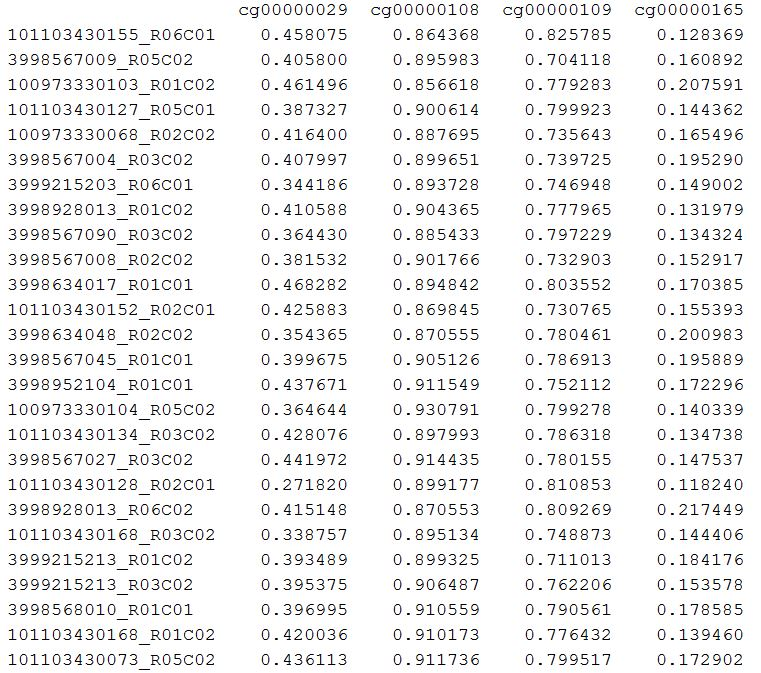
\includegraphics[scale=0.75]{images/pandas-example.JPG}
\caption{A truncated output of the \texttt{DataFrame} that stores the (shuffled) data set. We can use this output to study the information available in the \texttt{DataFrame}, and how this information is structured.}
\label{data:pandas:example}
\end{figure}

\section{Using SVMs} \label{data:svms}

For all numerical experiments described in chapter \ref{methods}, the SVM will be used, when there is a need for a classifier. For example, if the method used is a wrapper method, the SVM will be used to evaluate the performance of the feature subset. In contrast, in a filter method, the SVM will not come into play. This is similar to previous works such as \cite{RefWorks:216}, where the classifier is fixed, and attention is focused on the feature selection algorithms.

The SVM is fitted using the \texttt{scikit-learn} Python software \cite{scikit-learn}. Calling the \texttt{SVC()} method would create a classifier with default parameters, such as the default Radial Basis Function (RBF) kernel, and default error parameter $C=1.0$ (see section \ref{bg:ml:svm:model}). Alternatively, one can specify $C$ and the type of kernel.

A practical guide to SVMs by Hsu \textit{et. al} in \cite{RefWorks:128} argues that when the number of features is much larger than the number of samples, using a linear kernel would suffice, so the linear kernel will primarily be used in the experiments in chapter \ref{methods}.

%; in other words, we might not need to map our data into higher dimensions with an RBF kernel.

However, it is not sufficient to simply assume the default penalty parameter $C=1.0$. Instead, as Hsu \textit{et. al} suggested, performing a grid search on $C$ allows us to find an optimal $C$ that might perform better than the default value. However, due to time constraints, the following experiments would stick to the default value of $C$. Using other kernels and parameters is proposed as an extension in section \ref{further_work}.

%Moreover, this project focuses on the feature selection algorithms, not the parameters of the SVM.


\section{Cross validation}
The cross validation (CV) scores can be obtained via the \texttt{cross\_val\_score} method in the \texttt{sklearn.model\_selection} package. The number of folds used throughout this project is 5. That is, 80\% of samples will be used to train an SVM, while the other 20\% will be used on the newly-fit SVM to obtain an accuracy score. This is repeated 5 times, where the training/testing set in each iteration is unique. The CV score across all the folds is then the average classification accuracy across all five iterations. The cross validation process is illustrated in Figure \ref{data:cv}.

Fitting an SVM and obtaining CV scores using 5-fold cross validation with either the linear or RBF kernel took about 30 minutes each using the High Performance Computing cluster (see section \ref{hpc}) at Imperial College \cite{RefWorks:218}. All of the features were used in both cases.

The choice of 5 folds was also made in other works such as \cite{RefWorks:187}, while other works such as \cite{RefWorks:202} and \cite{RefWorks:212} use 10 folds. More folds will allow us to train and test the classifier more extensively, obtaining scores with higher accuracy. However, we note that \cite{RefWorks:202} investigated data sets with less than 20 features and the cross validation process will not take up a lot of time. On the other hand, due to the large number of features this project deals with, using 5 folds is a good balance between computational time and accuracy.

\begin{figure}
\centering

\usetikzlibrary{chains}
\makeatletter
\tikzset{
  on chain/.append code={
    \ifnum\c@pgf@counta=1\relax
      \tikzset{every first on chain/.try}%
    \fi
  },
  start chain/.append code={%
    \edef\pgf@marshal{\noexpand\tikzset{execute at end scope={\noexpand\xdef\noexpand\tikzpreviouschain{\tikz@lib@chain@name}}}}%
    \pgf@marshal
  }
}
\def\listset{\pgfqkeys{/List}}
\tikzset{
  no line/.style={font=\strut,text depth=+0pt,minimum width=+1.2em, inner xsep=+0pt},
  raw sort entry/.style={rectangle, thick, draw, font=\strut,text depth=+0pt,minimum width=+1.2em, inner xsep=+0pt},
  sort entry black/.style={raw sort entry, black, fill=white},
  sort entry blackgray/.style={raw sort entry, black, fill=gray!25},
  s1/.style={raw sort entry, fill=yellow!30},
  s2/.style={raw sort entry, fill=green!20},
  s3/.style={raw sort entry, fill=orange!25},
  g/.style={raw sort entry, fill=lightgray},
  h/.style={raw sort entry},
  no/.style={no line}
}
\listset{
  chain name/.initial=,
  do/.style={
    /utils/exec={\begin{scope}[start chain=\pgfkeysvalueof{/List/chain name}]},
    int/do/.list={#1},
    /utils/exec=\end{scope},
  },
  int/do/.code={%
    \pgfutil@ifnextchar[\tikz@List@int@@do{\tikz@List@int@@do[]}#1\pgf@stop
  }
}
\def\tikz@List@int@@do[#1]#2\pgf@stop{%
  \node[on chain={\pgfkeysvalueof{/List/chain name}},#1] {#2};
}

\begin{tikzpicture}[
  node distance=+1em and +0pt,
  outer xsep=+0pt,
  outer ysep=+0pt,
]
 \listset{chain name=r1,do={[g], [g], [g], [g], [h], [h], [h], [h], [h], [h], [h], [h], [h], [h], [h], [h], [h], [h], [h], [h]}}
 \tikzset{every first on chain/.style={below=of \tikzpreviouschain-begin}}
\listset{chain name=r2, do={[h], [h], [h], [h],[g], [g], [g], [g], [h], [h], [h], [h], [h], [h], [h], [h], [h], [h], [h], [h]}}
 \tikzset{every first on chain/.style={below=of \tikzpreviouschain-begin}}
 
 \listset{chain name=r3, do={[h], [h], [h], [h],[h], [h], [h], [h], [g], [g], [g], [g], [h], [h], [h], [h], [h], [h], [h], [h]}}
 \tikzset{every first on chain/.style={below=of \tikzpreviouschain-begin}}
 
 \listset{chain name=r4, do={[h], [h], [h], [h],[h], [h], [h], [h], [h], [h], [h], [h], [g], [g], [g], [g], [h], [h], [h], [h]}}
 \tikzset{every first on chain/.style={below=of \tikzpreviouschain-begin}}
 
 \listset{chain name=r5, do={[h], [h], [h], [h],[h], [h], [h], [h], [h], [h], [h], [h], [h], [h], [h], [h], [g], [g], [g], [g]}}
 \tikzset{every first on chain/.style={below=of \tikzpreviouschain-begin}}

\end{tikzpicture}
\caption{A diagram illustrating 5-fold cross-validation. In each iteration, 20\% of the data is ``held-out'' as the test set (grey boxes), while the rest is used as the training set (white boxes). The overall CV score is the average classification accuracy across all 5 iterations.}
\label{data:cv}
\end{figure}

\section{Data preprocessing}
% Shuffling the data (random_state) + rationale
% Normalise data before training on SVM classifier.
% Store shuffled data in data store.

Before the data set can be used for cross validation, it needs to be preprocessed first. Hsu \textit{et. al} also described the importance of \textit{scaling} our data before fitting an SVM. In particular, scaling the data would prevent features with large values from dominating those with smaller values. Scaling the features such that each feature has zero mean and unit variance is also recommended when using the \texttt{SVC()} (support vector classification) method. This procedure is also carried out in other works such as \cite{RefWorks:228}. In this project, the data was scaled with the \texttt{sklearn.preprocessing} package in \texttt{scikit-learn}, using the \texttt{scale} method.

Furthermore, the raw data was sorted based on the classification (target label) of each sample: the samples in the raw data set were ordered such that the cases (label 0) came first, followed by the controls (label 1). It is thus sensible to \textit{shuffle} the data such that the target labels would not be in any particular order. The cross validation process also partitions the data set into folds, and the process of fitting a classifier using the data set will be affected if the samples are ordered, since this will introduce bias. For example, one of the test sets might only contain samples in a particular class.

The shuffling was done using the \texttt{sklearn.utils.shuffle} method. The method also allows us to set the reproducibility of the shuffling. Furthermore, as discussed in section \ref{data:understanding}, once the entire data set and labels are shuffled, these are stored in a \texttt{DataStore}, and is retrieved when needed.



\section{Using all features} \label{data:all_features}

In the context of feature selection, it is only sensible to compare the performance of the feature selection algorithms to the situation where all the features are used in SVM classification.

%The hypothesis made by Hsu \textit{et. al} discussed above, where a linear kernel might suffice for data with high dimension, was tested on our data set.

Fitting an SVM using the RBF kernel with all the features produced a cross validation score of 0.834644, while with the linear kernel, the score was 0.929160. Nevertheless, this result does not necessarily mean that the linear kernel is more effective than the RBF kernel as suggested by Hsu \textit{et. al}, since some subsets might perform better with the RBF kernel than with the linear kernel. However, due to time constraints, only the linear kernel was used. As an extension, we can also investigate the performance of the RBF kernel with different subsets of features (see section \ref{further_work}).

\section{Investigating dependencies on other variables}

As mentioned in section \ref{intro:epi}, epigenetics can be interpreted as a ``window'' through which the external environment of an individual can alter his or her DNA. Thus, in analysing the data, we should be aware of other variables, known as \textit{confounding factors}, that might affect the classification of the samples. Confounding factors, such as gender and lifestyle, contribute to the dynamic nature of epigenetics \cite{RefWorks:78}.

From the relevant files\footnote{For example, the files available from \url{http://www.ncbi.nlm.nih.gov/geo/query/acc.cgi?acc=GSE84727}.}, we can also extract the \textit{gender} and \textit{age} information for most of our samples. We thus need to check if these confounding factors influence the classification of our samples.

\subsection{Effects of linear regression}
Linear regression was performed on the data set, where we take age and gender as the independent variables and the feature values as the dependent variable. We want to see if there is any relationship between age, gender and the features. Suppose we let $Y=\text{feature}$ and $X_1=\text{age}$, $X_2=\text{gender}$. Then, from \cite{RefWorks:219}, we have a linear model
\begin{align*}
y = \beta_0 + \beta_1 \, x_1 + \beta_2 \, x_2 + \epsilon
\end{align*}
where $\epsilon$ is an unobservable, random error with mean 0 and unknown variance $\sigma_\epsilon^2$. $\beta_0, \beta_1, \beta_2$ are the coefficients of the linear model.

The process of linear regression then finds the best estimates $\widehat{\beta}_i$ of $\beta_i$ for $i \in \left\lbrace 0,1,2 \right\rbrace$ by the \textit{method of least squares}, which minimises the square of $\epsilon$ for each sample:
\begin{align*}
\min \, \sum_{i=1}^N \epsilon_i^2 = \sum_{i=1}^N \left( y_i - \beta_0 - \beta_1x_{i1} - \beta_2x_{i2} \right)^2
\end{align*}
where $N$ is the number of samples, and $x_{ij}$ is the $i$-th sample of the $j$-th variable for $i \in [1,N]$ and $j \in \left\lbrace 1,2 \right\rbrace$. The method of least squares was performed by using the \texttt{LinearRegression} module in Python.

After the linear regression procedure, we obtain a \textit{fitted/predicted} value $\widehat{y}$ of $y$. That is,
\begin{align*}
\widehat{y_i} = \widehat{\beta_0} + \widehat{\beta_1} \, x_{i1} + \widehat{\beta_2} \, x_{i2}
\end{align*}

\subsection{Effects of the residuals}

Intuitively, the method of least squares minimises the difference between the actual and fitted value of $y$. This leads to the definition of the \textit{residual}:
\begin{align*}
e_i = y_i - \widehat{y}_i, \quad i=1,2,\dots,N
\end{align*}

From \cite{RefWorks:252}, the residual can generally be interpreted as the variation that is not explained by the fitted model. The resulting residuals are thus the variation in the features that is unexplained by age and gender. This means that we can use the residuals as our new ``data set'', which factors out age and gender from the original data set.

We again fit an SVM using the residuals:

\begin{figure}[h]
\begin{center}
    \begin{tabular}{| c | c | c | } \hline
      & Linear & RBF \\ \hline
    Original data set & 0.929160 & 0.834644 \\ \hline
	Residuals & 0.851158  & 0.799983 \\ \hline
    \end{tabular}
\end{center}
\end{figure}

From the table above, we can see that the CV scores do not differ significantly (about 3\% to 7\% difference). With the residuals, the SVM seems to have slightly lower classification accuracy. This suggests that age and gender only have a small influence on the classification of the samples.

We should also note that in the original data, the ages of about 200 individuals were missing. These individuals were removed from the samples for the linear regression procedure, resulting in about 600 samples in the residuals data set. Because it is preferable to have more samples when fitting SVMs, and because there is little difference in using the residuals, we will use the \textit{original} data set instead.




\chapter{Methods and approaches}
\label{methods}

This chapter outlines the feature selection algorithms with which this project has experimented. Chapter \ref{evaluation} will then present and discuss the numerical results that these algorithms have produced. 

\section{$t$-test} \label{t-test}

We first explore one popular feature selection method, the $t$-test. The $t$-statistic is commonly used to determine if the means of two populations are equal. In the context of feature selection, it can be used to quantify the \textit{relevance} of each feature with respect to the target labels.

The $t$-statistic and its corresponding $p$-value can be computed using the \texttt{ttest\_ind} method in the \texttt{scipy.stats} \cite{scipy} library. For example, we can calculate the $t$-statistic between two groups, 0 and 1. Using this method, the null hypothesis is that the means of groups 0 and 1 ($\mu_0$ and $\mu_1$ respectively) are equal. That is,
\begin{align*}
H_0: \mu_0 = \mu_1 \quad \text{vs.} \quad H_1: \mu_0 \neq \mu_1
\end{align*}

\texttt{ttest\_ind} will then perform a two-sided test, and return the value of the $t$-statistic and its $p$-value. Given two groups of samples $X_0$ and $X_1$, the $t$-statistic $T$ is:
\begin{align*}
T = \frac{\bar{x}_0 - \bar{x}_1}{\sqrt{\frac{s_0^2}{n_0} + \frac{s_1^2}{n_1}}}
\end{align*}
where, for $i \in \left\lbrace 0,1 \right\rbrace$, $\bar{x}_i$ denotes the mean value of $X_i$, $n_i$ denotes the number of samples in $X_i$, and $s_i^2$ denotes an estimate of the variance of $X_i$. Then, under the null hypothesis, $T$ has a $t$-distribution, with $\nu$ degrees of freedom \cite{RefWorks:219}, where
\begin{gather*}
\nu = \frac{\left( \frac{s_0^2}{n_0} + \frac{s_1^2}{n_1} \right)^2}{ M_0 + M_1 } \\
\quad M_0 = \frac{\left(\sfrac{s_0^2}{n_0}\right)^2}{n_0-1} \quad \text{and} \quad
M_1 = \frac{\left(\sfrac{s_1^2}{n_1}\right)^2}{n_1-1}
\end{gather*}

\subsection{Interpretation of $t$-test}
In the context of feature selection, for each feature, we have to group the samples according to their classification under this feature. This means that for each feature, samples whose classification is 0 will belong to group 0, and samples whose classification is 1 will belong to group 1.

Under the null hypothesis $H_0: \mu_0 = \mu_1$, the means of these two groups are the same. This implies that the feature values have no influence on the classification of the samples. Using \texttt{ttest\_ind}, a low $p$-value means that we have enough evidence to \textit{reject} $H_0$. Rejecting $H_0$ means that we are certain that a feature has significant contribution to the classification and is therefore highly relevant to the target labels. Thus, this method will select features whose $p$-values are significantly \textit{low}.

Once we have the $p$-values of all the features, we can decide how to use these values to select the features that we desire. We can either select the first $k$ features that have the \textit{lowest} $p$ values (i.e. most certain that $\mu_0 \neq \mu_1$), or choose a certain threshold and discard those features whose $p$-values exceed this threshold.

\subsection{Relevance and redundancy} \label{t_test:redundancy}

Evidently, since the SVM is not involved in the feature ranking process and since each feature is considered one at a time, we can classify this method as a \textit{univariate filter} method. As mentioned in section \ref{bg:fs:classification}, univariate filters are computationally efficient. In this case, the method iterates through each feature only once. The efficiency of this method can be further enhanced by tapping on its inherent parallelism, since we can compute the $t$-statistic of each feature independently from the others (see section \ref{body:parallel}).

Using \texttt{ttest\_ind}, the $t$-statistic and $p$-values were appended to a list $L$, and sorted in ascending order of $p$-value. Once we have obtained the sorted list, selecting $k$ features means we simply need to select the top $k$ features, an operation that is computationally cheap.

However, one stark drawback of this method is that $t$-test only considers each feature singly. Even though its design is simple compared to multivariate filters or wrappers, it is not possible to take redundancy into account \cite{RefWorks:217}, at least not in its basic implementation. $t$-test ranks the features according to the $t$-statistic (or the $p$-value), but redundant features are known to have similar rankings \cite{RefWorks:163}. As such, we might end up selecting highly ranked, but similar, features in our classification. For example, \cite{RefWorks:220} describes how redundant genes (features) might belong to the same biological pathway, when actually only a subset of those genes is needed to achieve the same prediction accuracy.

%While creating exploratory plots, such as in Figures \ref{body:t_test:fig} and \ref{body:t_test:fig_zoom}, we were able to select an optimal $k$. However, in these cases, we assumed that the value of $k$ is not declared beforehand. Hence, we have the liberty to select an optimal $k$ that is able to give us the best cross validation score. At the same time, including more features in our subset $S$ will incur higher computational costs for training and prediction, and might include features that have similar biological meaning. For example, \cite{RefWorks:220} describes how redundant genes (features) might belong to the same biological pathway, when actually only a subset of those genes is needed to achieve the same prediction accuracy.

%Suppose we want to obtain a very small feature subset, such as $k=100$, which has a smaller CV score than the full feature set. We will then need to accept a compromise. That is, we will have to accept that the smaller subset will have slightly poorer classification accuracy. Depending on the problem at hand, this might be acceptable, as long as we have a range of classification accuracy (e.g. $\pm 0.01$ of the accuracy with all the features included), within which the performance of the classifier is deemed to be satisfactory.



\subsection{Variation of $t$-test: A lazy version of Sequential Forward Selection} \label{body:sfs:lazy}

It is interesting to see if ranking each feature according to its individual cross validation (CV) score will differ significantly from the $t$-test method. In other words, instead of ranking features based on their $t$-statistic, we rank them based on their \textit{individual} CV score. In this context, individual CV score refers to the CV score obtained by the SVM when it is fitted with only one feature. Since this is a greedier and lazier version of Sequential Forward Selection (SFS), we call this method lazy SFS. Furthermore, unlike $t$-test, this variation of SFS can be classified as a wrapper method, since it uses the SVM to evaluate the features.

First, we iterate through each feature and fit an SVM using just that feature. So, the SVM is trained on one feature at a time only. Then, a list of CV scores is obtained. We then sort this list in descending order. Similarly to $t$-test, selecting $k$ features means selecting the top $k$ features in the sorted list. We also note that the lazy SFS also suffers from the same shortcoming as $t$-test, as both do not take redundancy of features into account.

\section{Recursive feature elimination} \label{body:rfe}

Next, we consider the RFE method, which was relatively straightforward to implement, using the \texttt{RFE} method in the \texttt{sklearn.feature\_selection} package. This method provides a convenient way to specify the number of ``steps'' that the algorithm should take when eliminating features that are deemed unimportant. This parameter specifies the number of features to eliminate in each iteration. As what was discussed in section \ref{bg:fs:rfe}, specifying a step size larger than 1 will cause the algorithm to consider nested subsets in each iteration.

The Python \texttt{feature\_selection} package in \texttt{sklearn} offers an RFE method:
\begin{center}
\texttt{RFE(estimator, n\_features\_to\_select=None, step=1, verbose=0)}
\end{center}

to perform RFE on our data set. We can specify the \texttt{step} parameter to be larger than 1 to ensure that the algorithm does not take too long to compute. With step size of 1, the algorithm will iterate through each feature, and remove only one feature at a time. It will then eliminate the feature with the lowest weight. This is obviously computationally intensive, especially if we specify a small \texttt{n\_features\_to\_select} parameter. Thus, the step size will vary according to the \texttt{n\_features\_to\_select} parameter. This is discussed in detail in section \ref{eval:rfe}.

\section{Restricted Forward Selection (RFS)} \label{body:rfs}

The pseudocode of the RFS algorithm \cite{deng1998omega} is listed in algorithm \ref{RFSAlgo} on page \pageref{RFSAlgo}. The RFS is a greedy heuristic search that only searches the features that are the most promising.

While SFS incrementally selects the best feature to include in our subset of selected features $S$ by considering \textit{all} remaining features that are not in $S$, RFS only considers a \textit{part} of these remaining features. The features that RFS consider in each iteration are those that produce the best CV score individually.

Suppose there are $M$ features in total. Firstly, RFS iterates through each feature and records its CV score by fitting an SVM with just one feature. A list $L$ is used to keep track of these scores. $L$ is then sorted. The feature with the best CV score is selected as the first feature (call it $f_1$). Then, in the second iteration, RFS iterates only half of $L$ and pairs each remaining feature with $f_1$ to form a pair, and an SVM is fitted using this pair of features. The best pair is then selected. In the third round, RFS will iterate through $M/3$ of these features. The best triple is selected and the process continues until $k$ features are selected. An example demonstrating this concept is shown in Table \ref{body:rfs:example}.

Since the RFS algorithm uses the SVM, it can be classified as a \textit{wrapper} method. Furthermore, since RFS uses the CV score as a heuristic to guide its search, it does not explicitly quantify relevance and redundancy.


\begin{table}
\centering
    \begin{tabular}{ | c | c | c | }
    \hline
    Iteration & Subsets considered & Subset selected $S$ \\
    \hline
    1 & $f_1, f_2, \dots, f_M$ & $\left\lbrace f_3 \right\rbrace$ \\ \hline
    2 & $\left\lbrace f_3, f_1 \right\rbrace, \left\lbrace f_3, f_2 \right\rbrace, \left\lbrace f_3, f_4 \right\rbrace, \dots , \left\lbrace f_3, f_{M/2} \right\rbrace$ & $\left\lbrace f_3, f_1 \right\rbrace$ \\ \hline
    3 & $\left\lbrace f_3, f_1, f_2 \right\rbrace, \left\lbrace f_3, f_1, f_4 \right\rbrace, \dots , \left\lbrace f_3, f_1, f_{M/3} \right\rbrace$ & $\left\lbrace f_3, f_1, f_5 \right\rbrace$ \\ \hline
    \end{tabular}
\caption{A diagram demonstrating how the first three iterations of RFS work. Suppose the features $f_3, f_1, f_5$ are the top three features.}
\label{body:rfs:example}
\end{table}


\subsection{Runtime}
In the first iteration of the algorithm, all $M$ features are evaluated. In the second iteration, $M/2$ features are evaluated. Suppose this continues for $2^n$ iterations.

Then, we can calculate the number of features the algorithm evaluates:
\begin{align*}
M+\frac{M}{2}+\frac{M}{3}+\dots+\frac{M}{2^n} = M\left[ 1+\frac{1}{2}+\dots+\frac{1}{2^n} \right]=M \sum_{j=1}^{2^n} \frac{1}{j}
\end{align*}

It is a well-known result that the series $\sum_{i=1}^{\infty} \sfrac{1}{i}$ diverges, but we can attempt to obtain an upper bound of the sum above. We can split the sum above into $n$ groups, where the number of elements in the $p$-th group is $2^{p-1}$.

\begin{align*}
\sum_{j=1}^{2^n} \frac{1}{j}
&= 1 + \underbrace{\left[ \frac{1}{2} + \frac{1}{3} \right]}_{\text{Group 2}} + \underbrace{\left[ \frac{1}{4} + \frac{1}{5} + \frac{1}{6} + \frac{1}{7} \right]}_{\text{Group 3}} + \dots + \underbrace{\left[ \frac{1}{2^{n-1}} + \frac{1}{2^{n-1}+1} \dots + \frac{1}{2^{n}-1} \right]}_{\text{Group $n$}} + \frac{1}{2^n} \\
&< 1 + \left[ \frac{1}{2} + \frac{1}{2} \right] + \left[ \frac{1}{4} + \frac{1}{4} + \frac{1}{4} + \frac{1}{4} \right] + \dots + \left[ \frac{1}{2^{n-1}} + \dots + \frac{1}{2^{n-1}} \right] + \frac{1}{2^n} \\
&= 1+1+1+ \dots + 1 + \frac{1}{2^n} \\
&= n + \frac{1}{2^n}
\end{align*}

Now, let $k=2^n$, so $k>0$ and $n=\log k$ (the logarithm here implicitly has base 2).
\begin{align*}
\sum_{j=1}^k \frac{1}{j} < \log k+ \frac{1}{k} < \log k
\end{align*}

Thus, the total number of evaluations made by RFS is
\begin{align*}
M \sum_{j=1}^k \frac{1}{j} < M \log k
\end{align*}
where $k$ is the number of features that the algorithm selects. So, the RFS algorithm is executed in $\mathcal{O}(M\log k)$ (ignoring the complexity of the SVM classification).

In contrast, the SFS algorithm iterates through the whole feature set in each iteration. So, its complexity would be $\mathcal{O}(Mk)$. In the limit, if we want SFS to iterate through all the features, instead of terminating with $k$ features, the runtime complexity of SFS would be $\mathcal{O}(M^2)$ while that of RFS is $\mathcal{O}(M\log M)$.

It is evident that since RFS is a greedier variant  of SFS, the solution returned by RFS would most likely be less optimal than that by SFS. However, we need to find a balance between computational complexity and optimality of our solution. As $M$ is large in this case, the time complexity of the RFS would be helpful in selecting $k$ features within a reasonable amount of time despite its compromise in optimality.


\section{Maximum relevance minimum multi-collinearity (MRmMC)} \label{mrmmc}

Recently, MRmMC \cite{RefWorks:187} was proposed as a filter method to overcome the drawbacks and computational efforts required when using mutual information as a heuristic to quantify relevance and redundancy. MRmMC also does not require any parameter. Unlike RFE and RFS, MRmMC does not directly use CV scores to quantify relevance and redundancy. 


\subsection{Relevance}
% Use of conditional expectation to measure relevance.
% Use of coefficient of determination to measure redundancy.
% Coefficient of determination

MRmMC uses a correlation coefficient, first used in \cite{RefWorks:188}, to quantify the relevance of each feature to the target class. For random variables $X$ and $Y$, this correlation coefficient is:
\begin{align*}
r_{qn}(X, Y) = \left( 1 - \frac{E_Y[\var_X(X|Y)]}{\var(X)} \right)^{\frac{1}{2}}
\end{align*}


This measure is motivated by some definitions and properties of conditional probabilities:\\

\begin{mydef}[Expectation]
\label{mrmmc:def:ex}
The expectation of a discrete random variable $X$ is:
\begin{align*}
E[X] = \sum_{x \in X} x P(X=x)
\end{align*}
\end{mydef}

\begin{mydef}[Marginal expectation]
\label{mrmmc:def:margex}
The marginal expectation of a discrete random variable $X$, in terms of its conditional expectation given another discrete random variable $Y$, is:
\begin{align*}
E[X] = \sum_{y \in Y} P(Y=y) \, E_X[X \, | \, Y=y]
\end{align*}
where $E_X$ denotes expectation with respect to $X$. That is,
\begin{align*}
E_X[X \, | \,Y=y] = \sum_{x\in X} x \, P(X=x \, | \, Y=y)
\end{align*}
\end{mydef}

\begin{mydef}[Marginal variance]
\label{mrmmc:def:margvar}
The marginal variance of $X$ is:
\begin{align*}
\var(X) = E[X^2] - \left( E[X] \right) ^2
\end{align*}
\end{mydef}

The definition of marginal variance can be extended to the conditional variance.\\

\begin{mydef}[Conditional variance]
The conditional variance of $X$, given $Y$, is:
\begin{align*}
\var_X(X \, | \, Y) = E_X[X^2 \, | \, Y] - \left( E_X[X \, | \, Y] \right)^2
\end{align*}
\end{mydef}

Since the conditional variance is a random variable with respect to $Y$, we can find the expectation of the quantity:
\begin{align}
E_Y [ \var_X(X \, | \, Y) ] = E_YE_X[X^2 \, | \, Y] - E_Y [ E_X(X\,|\,Y) ] ^2 \label{mrmmc:eq:star}
\end{align}

By definition \ref{mrmmc:def:ex}, we can show that:
\begin{align}
E_YE_X[X \, | \, Y] &= \sum_{y \in Y} P(Y=y) \, E_X[X \, | \, Y=y] = E[X] \label{mrmmc:eq:exp1} \\
\Rightarrow E_YE_X[X^2|Y] &= E[X^2] \nonumber
\end{align}

From equation \ref{mrmmc:eq:star},
\begin{align}
\Rightarrow E_Y [ \var_X(X \, | \, Y) ] &= E[X^2] - E_Y [ E_X(X\,|\,Y) ] ^2 \label{mrmmc:eq:exp2}
\end{align}

Now, we also consider the variance with respect to $Y$ of the conditional expectation:
\begin{align}
\var_Y (E_X[X \, | \, Y]) &= E_Y \left( E_X[X \, | \, Y]\right)^2 - \left( E_YE_X[X \, | \, Y] \right)^2 \nonumber \\
&= E_Y \left( E_X[X \, | \, Y]\right)^2 - \left( E[X] \right)^2 \label{mrmmc:eq:exp3}
\end{align}
where we used the result from equation \ref{mrmmc:eq:exp1}. Then, rearranging equation \ref{mrmmc:eq:exp3} and combining with equation \ref{mrmmc:eq:exp2}, we get:
\begin{align*}
E_Y [ \var_X(X \, | \, Y) ] &= E[X^2] - \var_Y (E_X[X \, | \, Y]) - \left( E[X] \right)^2 \\
&= \var(X) - \var_Y (E_X[X \, | \, Y]) \\
\Rightarrow \var(X) &= \var_Y (E_X[X \, | \, Y]) + E_Y [ \var_X(X \, | \, Y) ]
\end{align*}
where we used the definition of marginal variance in definition \ref{mrmmc:def:margvar}.

Thus, as discussed in \cite{RefWorks:187}, the variance of the random variable $X$ is made of two parts: $\var_Y (E_X[X \, | \, Y])$ and $E_Y [ \var_X(X \, | \, Y) ]$. The latter describes the average variability with respect to different targets: on average, how much do the feature values vary with different targets?

%\begin{itemize}
  %\item $\var_Y (E_X[X \, | \, Y])$ describes the variability between the targets (or outcomes): how much do the targets deviate from its mean with the feature values?
  
  %\item $E_Y [ \var_X(X \, | \, Y) ]$ describes the average variability with respect to different targets: on average, how much do the feature values vary with different targets?
%\end{itemize}

Using $X$ as our feature and $Y$ as the target label, $E_Y[\var_X(X|Y)]$ is used in measuring the relevance of the feature and its classification.

\subsection{Properties of correlation coefficient}
A mathematically convenient property of the correlation coefficient
\begin{align*}
r_{qn}(X, Y) = \left( 1 - \frac{E_Y[\var_X(X|Y)]}{\var(X)} \right)^{\sfrac{1}{2}}
\end{align*}

is that $0 \leq r_{qn}(X, Y) \leq 1$. First, we define independence between two variables:\\

\begin{mydef}[Independence]
Two random variables $X$ and $Y$ are independent iff
\begin{align}
P(X, Y) = P(X) \, P(Y) \label{mrmmc:eq:indep}
\end{align}
where $P(X, Y)$ denotes the joint probability of $X$ and $Y$.
\end{mydef}

In $r_{qn}(X,Y)$,
\begin{align*}
E_Y[\var_X(X|Y)]
&= E[X^2] - E_Y\left( E_X(X|Y) \right)^2 \quad \text{(by eqn \ref{mrmmc:eq:exp2})} \\
&= E[X^2] - \sum_{y\in Y} P(Y=y) \left[ E_X(X|Y=y) \right]^2 \quad \text{(by defn \ref{mrmmc:def:margex})} \\
&= E[X^2] - \sum_{y\in Y} P(Y=y) \left[ \sum_{x \in X} x \, P(X=x|Y=y) \right]^2 \\
&= E[X^2] - \sum_{y\in Y} P(Y=y) \left[ \sum_{x \in X} x \, \frac{P(X=x, Y=y)}{P(Y=y)} \right]^2
\end{align*}

Assuming $X$ and $Y$ are independent, we can apply equation \ref{mrmmc:eq:indep}:
\begin{align*}
E_Y[\var_X(X|Y)]
&= E[X^2] - \sum_{y\in Y} P(Y=y) \left[ \sum_{x \in X} x \, \frac{P(X=x) \, P(Y=y)}{P(Y=y)} \right]^2 \\
&= E[X^2] - \sum_{y\in Y} P(Y=y) \left[ \sum_{x \in X} x \, P(X=x) \right]^2 \\
&= E[X^2] - \underbrace{\sum_{y\in Y} P(Y=y)}_{=1} \left[ E(X) \right]^2 \\
&= \var(X) \\
\Rightarrow r_{qn}(X,Y) &= 0
\end{align*}

So, $r_{qn}(X, Y)$ attains its lower bound when $X$ and $Y$ are \textit{independent}. On the other hand, $r_{qn}(X, Y)$ approaches 1 when $X$ and $Y$ are strongly correlated, according to \cite{RefWorks:187}. In the limit, suppose $X$ is a function of $Y$: $Y=f(X)$. Then, given $Y=y$, we can find the value of $X=x$ and vice versa. In other words, we can deterministically find the value of one variable given the other. Thus,

\begin{align*}
E_Y[\var_X(X|Y)]
&= E_Y [E_X(X^2|Y)-\left( E_X(X|Y) \right)^2 ] \quad \text{(by defn \ref{mrmmc:def:margvar})} \\
&= \sum_{y \in Y} P(Y=y) \left[ E_X(X^2|Y=y)- ( E_X(X|Y=y))^2 \right] \\
&= \sum_{y \in Y} P(Y=y) \left[E_X\left(x^2\right)-\left( E_X\left(x \right) \right)^2 \right] \\
&= \sum_{y \in Y} P(Y=y)  \left[x^2 -x^2 \right] , \quad \text{since $x$ is non-random} \\
&= 0 \\
\Rightarrow r_{qn} (X, Y) &= 1
\end{align*}

As such, MRmMC aims to find features in the set $F$, that are strongly relevant to the target class, by \textit{maximising} $r_{qn}$ between each feature $f$ and the target labels $c$. That is,
\begin{align*}
\argmax_{f \in F} \quad r_{qn}(f, c)
\end{align*}

\subsection{Computing relevance}
Now, we see how the terms in $r_{qn}$ can be computed using the raw data. From equation \ref{mrmmc:eq:exp2},
\begin{align*}
E_Y [ \var_X(X \, | \, Y) ]
&= E[X^2] - E_Y [ E_X(X\,|\,Y) ] ^2 \\
&= E[X^2] - \sum_{y \in Y} P(Y=y) \left[ E_X(X|Y=y) \right]^2 
\end{align*}

In the context of our data, $X$ represents the features and $Y$ represents the target labels. For our data, binary target classes are used: $Y= \left\lbrace 0,1 \right\rbrace$. So, we can expand the above:
\begin{align*}
E_Y [ \var_X(X \, | \, Y) ]
= E[X^2] &- P(Y=1) \left[ E_X(X|Y=1) \right]^2 - P(Y=0) \left[ E_X(X|Y=0) \right]^2 
\end{align*}

The expectations above and the variance term in the denominator of $r_{qn}$ can be computed using unbiased estimators of expectation and variance respectively:
\begin{align*}
E(X) = \bar{x} \approx \frac{1}{n} \sum_{x \in X} x \quad \text{and} \quad \var(X) \approx \frac{1}{n-1} \sum_{x \in X} (x- \bar{x})^2
\end{align*}

To compute the conditional expectation $E_X(X|Y=y)$, we simply compute the expectation of those realisations of $X$ whose corresponding realisation of $Y$ is $y$. To compute $P(Y=y)$, we simply have to count how frequent $y$ appears as a realisation of $Y$ throughout the cases.

A simple example below shows how we could compute the probabilities discussed above:

\begin{center}
    \begin{tabular}{| c || c | c |}
    \hline
     Case & $X$ & $Y$ \\ \hline \hline
     1 & 0.5 & 1 \\ \hline
     2 & 0.2 & 0 \\ \hline
     3 & 0.1 & 1 \\ \hline
    \end{tabular}
\end{center}

In this case,
\begin{align*}
E_X(X|Y=1) &= \frac{1}{2} \,  (0.5+0.1) = 0.3 \quad \text{(Expectation of $X$ over cases 1 and 3)} \\
P(Y=1) &= \frac{2}{3} \\
E[X^2] &= \frac{1}{3} \, (0.5^2+0.2^2+0.1^2) = 0.1 \\
E[X] &= \frac{1}{3} \, (0.5+0.2+0.1) \approx 0.2666 \\
\var(X) &= E[X^2] - (E[X])^2 \approx 0.02892
\end{align*}

As such, we can employ the same method to compute the required expectations and variances for our data. To make this task simpler, we utilise methods in the \texttt{numpy} \cite{RefWorks:214} package: the \texttt{mean} and \texttt{var} methods are used to compute expectation and variance respectively.

\subsection{Redundancy and multicollinearity}

Multicollinearity, in the context of feature selection, refers to a strong correlation between features \cite{RefWorks:234}.

MRmMC uses the \textit{squared multiple correlation coefficient} (call it $R^2$) to quantify the degree of redundancy between features. The $R^2$ term between a dependent variable and an independent variable can be interpreted as the \textit{proportion of the variance of the dependent variable explained by the independent variable} \cite{RefWorks:193}. In other words, if $R^2$ is high, then a high proportion of the dependent variable's variance can be extracted from the independent variable. Therefore, the dependent variable is highly redundant.

Assume there exists a set of vectors $Q=\left\lbrace q_1, q_2, \dots, q_k \right\rbrace$ where the vectors are \textit{pairwise orthogonal}. That is, $\forall i,j = 1, \dots, k$,
\begin{align*}
q_i \cdot q_j = q_i^\top q_j = 0, \quad i \neq j 
\end{align*}

A useful property of $R^2$ is that, the $R^2$ term between a variable $f$ and $Q$ is the \textit{sum} of $R^2$ between each $q \in Q$ and $f$ \cite{RefWorks:193}. That is,
\begin{align*}
R^2(Q, f) = \sum_{i=1}^k R^2(q_i, f), \quad q_i \in Q
\end{align*}

This is useful when computing $R^2$ between one variable and a \textit{group} of pairwise orthogonal variables.

In \cite{RefWorks:187}, the $R^2$ term used in MRmMC is defined as such: Suppose there exists a feature set $S$ with features $\left\lbrace f_1 , \dots , f_{k-1} \right\rbrace$, with corresponding orthogonal components $Q= \left\lbrace q_1, \dots , q_{k-1} \right\rbrace$, where $f_i, q_i \in \mathbb{R}^n$ for $i=1, \dots, k-1$. Suppose we are considering a new feature $f$. Then, for any orthogonal component $q \in Q$,
\begin{align}
R^2(f, q) = \frac{\left( \sum_{i=1}^n f_iq_i \right)^2}{\left(\sum_{i=1}^n f_i^2 \right) \left( \sum_{i=1}^n q_i^2 \right)} \label{mrmmc:r2}
\end{align}

where $f_i,q_i$ refers to the $i$-th element of the vectors $f$ and $q$ respectively, where $i=1, \dots , n$.

Since the components of $Q$ are pairwise orthogonal, the $R^2$ term of the new vector $f$ and all the components of $Q$ would be the sum of the $R^2$ terms:
\begin{align*}
R^2(f, Q) = \sum_{i=1}^{k-1} R^2(f, q_i), \quad q_i \in Q
\end{align*}

Furthermore, $R^2$ can be interpreted as the square of the \textit{Pearson correlation coefficient} $\rho$ of vectors $x,y \in \mathbb{R}^n$:
\begin{align*}
\rho(x, y) = \frac{\sum_{i=1}^n (x_i - \bar{x})(y_i - \bar{y})}{\sqrt{\sum_{i=1}^n (x_i-\bar{x})^2}\sqrt{\sum_{i=1}^n (y_i-\bar{y})^2}}
\end{align*}
where $\bar{x}$ and $\bar{y}$ denote the mean of $x$ and $y$ respectively. We can see that the square of $\rho$ would equal to the $R^2$ term in equation \ref{mrmmc:r2} when the means of $f$ and $q$ are zero. Thus, we need to ensure that $f$ and $q$ have zero mean for the above interpretation to work.

As mentioned above, since we would like to reduce the redundancy between features, we would need to \textit{minimise} $R^2$ between $f$ and the previously selected features.\\

Therefore, for an orthogonal set $Q$ and target labels $c$, the algorithm will select feature $f$ that maximises the following criterion:
\begin{align*}
J(f, Q) = r_{qn}^2(f, c)- \sum_{i=1}^{k-1} R^2(f, q_i), \quad q_i \in Q
\end{align*}
where the orthogonal set $Q$ is obtained by orthogonalising the set of selected features.

Note that the $r_{qn}$ term is squared so that both terms in the equation are squared. Overall, the pseudocode for MRmMC can be found in Algorithm \ref{MRmMCAlgo}.

\begin{algorithm}
\DontPrintSemicolon
\KwIn{Data set $D$ with $M$ features.}
\KwOut{Subset $S$ ($S \subset D$) of the $M$ features such that $|S|=k$, $k \ll M$.}
\BlankLine
\Begin{
Initialise empty list $S \longleftarrow [\,]$ \;
Initialise empty list $Q \longleftarrow [\,]$ \;
\For{$i=1 \longrightarrow M$}{
Compute $r_{qn}^2(f_i, c)$ for $i$-th feature, $f_i$ and target labels $c$. \;
}
$w \longleftarrow $ feature with maximum $r_{qn}^2$. \;
$S \longleftarrow S \cup \left\lbrace w \right\rbrace$ \;
$Q \longleftarrow Q \cup \left\lbrace w \right\rbrace$ \;
\BlankLine
\For{$h=2 \longrightarrow k$}{
\For{each feature $f_i$ not in $S$} {
Compute $J(f_i) = r_{qn}^2(f_i, c) - \sum_{j=1}^{h-1} R^2(f_i, q_j)$, where $q_j \in Q$. \;
}
$w \longleftarrow $ feature with maximum $J$. \;
$S \longleftarrow S \cup \left\lbrace w \right\rbrace$ \;
$Q \longleftarrow Q \cup \left\lbrace w \right\rbrace$ \;
Orthogonalise $Q$. \;
}
}
\caption{MRmMC($D$, $k$) \label{MRmMCAlgo}}
\end{algorithm}

\subsection{Computing redundancy} \label{mrmmc:redundancy:computation}

The MRmMC paper \cite{RefWorks:187} derives the orthogonal vector $q_k$ of $f_k$ with respect to a set of orthogonal vectors $Q = \left\lbrace q_i: i \in [1, k-1] \right\rbrace$ via:
\begin{align*}
q_k = f_k  - \frac{f_k^\top q_1}{q_1^\top q_1}q_1  - \frac{f_k^\top q_2}{q_2^\top q_2}q_2 - \dots - \frac{f_k^\top q_{k-1}}{q_{k-1}^\top q_{k-1}}q_{k-1}
\end{align*}

This is evidently the \textit{classical Gram-Schmidt} (CGS) process. However, CGS is notable for its numerical instability because there is usually a loss of orthogonality in the resulting $q_k$ vectors \cite{RefWorks:195}. Instead, other methods such as the \textit{modified Gram-Schmidt} (MGS) or \textit{Householder transformations} are preferred.

%Although there are several algorithms in the literature of linear algebra, such as Householder transformations, that alleviate the problem of instability of CGS, this project will not delve further into these algorithms, but instead simply use MGS to compute the set of orthogonal vectors $Q$. Besides, \cite{RefWorks:194} also notes that MGS is almost as numerically stable as algorithms that use Householder transformations.

The computation of $Q$ was performed using the \texttt{numpy.linalg.qr} method. This method returns an \textit{orthonormal} matrix and an upper triangular matrix $\boldsymbol R$ that does not play a role in computing $R^2$. An orthonormal matrix has orthonormal columns, which are orthogonal columns with a magnitude (2-norm) of 1. This would not affect the computation of $R^2$:

%The pseudocode in algorithm \ref{MGS}, from \cite{RefWorks:195}, outlines the procedure for MGS. We also note that MGS produces an upper triangular matrix $\boldsymbol R$ that does not play a role in computing $R^2$. Furthermore, the original matrix $A$ in algorithm \ref{MGS} is overwritten by \textit{orthonormal} columns, which are orthogonal columns with the added constraint that they have a magnitude (2-norm) of 1. This would not affect how $R^2$ is used as described above.

\begin{proof}
Suppose we have an arbitrary vector $q \in \mathbb{R}^n$ and a normalised vector $\tilde{q} \in \mathbb{R}^n$ such that $\tilde{q} = \sfrac{q}{\| q \|_2}$. Then,
\begin{align*}
R^2(f, \tilde{q}) = \frac{\left( \sum_{i=1}^n f_i \tilde{q}_i \right)^2}{\left(\sum_{i=1}^n f_i^2 \right) \left( \sum_{i=1}^n \tilde{q}_i^2 \right)}
= \frac{\left( f^\top \tilde{q} \right)^2}{(f^\top f)(\tilde{q}^\top \tilde{q})}
= \frac{\frac{1}{\| q \|^2_2} \left( f^\top q \right)^2}{(f^\top f) \cdot \frac{1}{\| q \|^2_2} \left( q^\top q \right)} = R^2(f, q)
\end{align*}
\end{proof}

Thus, the computation of the $R^2$ term using orthonormal vectors will still be valid.


\begin{comment}
\begin{algorithm}
\DontPrintSemicolon
\KwIn{Matrix $A\in \mathbb{R}^{m \times n}$, with columns $A_k$ where $k \in [1,n]$.}
\KwOut{Matrix $A\in \mathbb{R}^{m \times n}$ with orthonormal columns.}
\BlankLine
\Begin{
\For{$k=1 \longrightarrow n$}{
$R(k, k) = \| A_k \|_2$ \;
$Q_k = \sfrac{A_k}{R(k, k)}$ \;
\For{$j=k+1 \longrightarrow n$}{
$R(k, j)  =  Q_k^\top A_j$ \;
$A_j = A_j - Q_k \times R(k, j) $ \;
}
}
}
\caption{Modified Gram-Schmidt Orthogonalisation($A$) \label{MGS}}
\end{algorithm}
\end{comment}

\subsection{Implementing MRmMC}

Two versions of MRmMC were implemented. The first incorporates the idea of Restricted Forward Selection (RFS). This truncated version only considers part of the features that have the highest $r_{qn}$ (i.e. the top $k$ features with the best individual $r_{qn}$), whereas the full version considers every feature that has not been already selected.

The truncated version considers all of the features in its first iteration, half of the features in the second iteration, one third of the features in the third iteration and so on. This is similar to RFS. Evidently, this will cause optimality to suffer, but the computation process will terminate much quicker.

The results are discussed in chapter \ref{evaluation}.

\section{MRmMC issues} \label{mrmmc:issues}

The challenges of implementing MRmMC arise mainly due to the high dimensionality of the data set. In the MRmMC paper \cite{RefWorks:187}, the data sets that were experimented on had at most 216 features, and had many more samples than features. For example, one data set had 2000 samples and 216 features.

\subsection{Problems with computing redundancy} \label{mrmmc_probs}

From algorithm \ref{MRmMCAlgo}, we can see that the matrix of orthogonal vectors $Q$ expands with the number of features considered in the step $Q \longleftarrow Q \cup \left\lbrace w \right\rbrace$. For example, after selecting the first feature, $Q \in \mathbb{R}^{n \times 1}$, where $n$ is the number of samples in the data set. In the next iteration, a vector is appended to $Q$ such that $Q \in \mathbb{R}^{n \times 2}$ and $Q$ is converted to an orthonormal matrix. This continues until we reach the desired number of features $k$.

However, from \cite{RefWorks:253}, we note that this orthogonalisation process can be interpreted as constructing an \textit{orthonormal basis} for a \textit{subspace} of $\mathbb{R}^{n}$.

Suppose the set $Q$ contains $n$ feature vectors. That is, $Q \in \mathbb{R}^{n \times n}$. Then, the vectors of $Q$ can be interpreted as a basis for the space $\mathbb{R}^{n}$. In other words, any vector $u \in \mathbb{R}^{n}$ can be formed by a linear combination of the vectors in $Q$.

Consequently, attempting to append another vector $v \in \mathbb{R}^{n}$ and orthogonalising the resulting matrix will render $v$ redundant, as the space $\mathbb{R}^{n}$ can be constructed solely based on the previous $n$ vectors in $Q$, without the additional $v$. Thus, we will not be able to orthogonalise a matrix $Q \in \mathbb{R}^{n \times (n+1)}$. This problem will occur if the number of features to be selected by the feature selection algorithm exceeds the number of samples in the data set. Indeed, we see that in the original MRmMC paper, MRmMC was performed on data sets which have fewer features than samples, unlike the case for our data set. So, this problem will not occur for the data sets used in the MRmMC paper.

This means that, for our data set, the algorithm should only select at most 847 features. The result of choosing 847 features is discussed in chapter \ref{evaluation}. This limitation will put a heavy restriction on the feature selection process. Thus, instead of using the $R^2$ measure for redundancy, we can instead incorporate genetic algorithms while using the $r_{qn}$ quantity.

\subsection{Computational complexity}

We first note that the MRmMC method is a filter method since it does not employ the SVM at all. A common benefit of filter methods is its computational efficiency. For example, the $t$-test only needs to compute the $t$-statistic of each feature once. Despite its classification as a filter method, MRmMC is not as computationally efficient, especially when a lot of features are involved.

Computational effort is mostly spent in computing the QR factorisation of the selected features. This is for the purpose of quantifying the redundancy among the selected features. According to \cite{RefWorks:253}, the CGS algorithm used to compute the orthgonal vectors has complexity $\mathcal{O}(mn^2)$ for a matrix $Q \in \mathbb{R}^{m \times n}$. That is, the complexity of the algorithm grows quadratically with features, versus the linear time complexity offered by $t$-test. So, with more features, the algorithm will take a longer time to compute the QR factorisation of the matrix $Q$.

Thus, not using the $R^2$ term will allow us to avoid this computational complexity, which gives us a stronger reason to use genetic algorithms instead.

%Incorporating the GA will avoid the above time complexity.

%In general, we see that the GA does not require many number of iterations to converge for this data set, and its cross validation scores are similar compared to $t$-test.


\section{Integrating genetic algorithm with MRmMC} \label{ga:mrmmc}

As mentioned in section \ref{bg:fs:ga}, genetic algorithms (GAs) are popular in the literature of feature selection. The GA implemented in this project defines the \textit{fitness} of the chromosomes based on their CV scores. The $r_{qn}$ measure is also used in a two-stage variant of the GA.


\subsection{Parameters and strategies}
\label{body:ga:params}

Due to the large number of features in the epigenetics data set, this project uses the ``two-stage'' GA, as illustrated in Figures \ref{bg:fs:ga:twoStage} and \ref{bg:ga:twostage:diag}.

We first use the correlation coefficient $r_{qn}$ to choose the best features in the first stage of the GA. Alternatively, we could also use the classification score of each feature on an SVM as a guide to eliminate features that might not be relevant to the target class, as used in RFS. We choose the former. Once we have a list of the $r_{qn}$ values, we sort it, and obtain the top $s$ features. This set of features is the result of the initial filtering of the algorithm. This forms the first stage of the GA, as shown in Figure \ref{bg:ga:twostage_a}.

Then, from the top $s$ features, we randomly select $k$ features that will form the solutions in the first generation of the GA. The presence of a feature is encoded by a `1', while its absence is encoded by a `0'. This is done until there are $G$ solutions in the generation. This is shown in Figure \ref{bg:ga:twostage_b}.

%So, assume $s=2000$ and $k=1000$. Only 1000, out of the 2000 features selected by the first stage, will form a solution. 

Figure \ref{bg:ga:twostage:diag} demonstrates this two-stage GA with 20 features in total. In this case, $M=20$, $s=9$ and $k=5$.


\begin{figure}
\centering

\usetikzlibrary{chains}
\makeatletter
\tikzset{
  on chain/.append code={
    \ifnum\c@pgf@counta=1\relax
      \tikzset{every first on chain/.try}%
    \fi
  },
  start chain/.append code={%
    \edef\pgf@marshal{\noexpand\tikzset{execute at end scope={\noexpand\xdef\noexpand\tikzpreviouschain{\tikz@lib@chain@name}}}}%
    \pgf@marshal
  }
}
\def\listset{\pgfqkeys{/List}}
\tikzset{
  no line/.style={font=\strut,text depth=+0pt,minimum width=+1.2em, inner xsep=+0pt},
  raw sort entry/.style={rectangle, thick, draw, font=\strut,text depth=+0pt,minimum width=+1.2em, inner xsep=+0pt},
  dotted entry/.style={rectangle, dashed, draw, font=\strut,text depth=+0pt,minimum width=+1.2em, inner xsep=+0pt},
  sort entry black/.style={raw sort entry, black, fill=white},
  sort entry blackgray/.style={raw sort entry, black, fill=gray!25},
  s1/.style={raw sort entry, fill=yellow!30},
  s2/.style={raw sort entry, fill=green!20},
  s3/.style={raw sort entry, fill=orange!25},
  g/.style={raw sort entry, fill=lightgray},
  h/.style={raw sort entry},
  d/.style={dotted entry},
  no/.style={no line}
}
\listset{
  chain name/.initial=,
  do/.style={
    /utils/exec={\begin{scope}[start chain=\pgfkeysvalueof{/List/chain name}]},
    int/do/.list={#1},
    /utils/exec=\end{scope},
  },
  int/do/.code={%
    \pgfutil@ifnextchar[\tikz@List@int@@do{\tikz@List@int@@do[]}#1\pgf@stop
  }
}
\def\tikz@List@int@@do[#1]#2\pgf@stop{%
  \node[on chain={\pgfkeysvalueof{/List/chain name}},#1] {#2};
}

\begin{subfigure}[b]{\textwidth}
\centering
\begin{tikzpicture}[
  node distance=+1em and +0pt,
  outer xsep=+0pt,
  outer ysep=+0pt,
]
 \listset{chain name=r1,do={[h], [h], [h], [h], [h], [h], [h], [h], [h], [d], [d], [d], [d], [d], [d], [d], [d], [d], [d], [d]}}
 \tikzset{every first on chain/.style={below=of \tikzpreviouschain-begin}}
      
\end{tikzpicture}
\caption{First stage of GA. Suppose the entire array represents all the features. The solid boxes represent those features that have high $r_{qn}$ and thus considered for the GA, while the dotted boxes are those features that are not considered for the GA. Hence, only the features represented by the solid boxes will appear in a solution of the GA.}
\label{bg:ga:twostage_a}
\end{subfigure}\\[2em]

\begin{subfigure}[b]{\textwidth}
\centering
\begin{tikzpicture}[
  node distance=+1em and +0pt,
  outer xsep=+0pt,
  outer ysep=+0pt,
]
 \listset{chain name=r1,do={[h]0, [h]1, [h]1, [h]1, [h]0, [h]0, [h]1, [h]0, [h]1, [d], [d], [d], [d], [d], [d], [d], [d], [d], [d], [d]}}
 \tikzset{every first on chain/.style={below=of \tikzpreviouschain-begin}}
      
\end{tikzpicture}
\caption{Second stage of GA. A solution is generated by assigning either 0 or 1 to each feature. This diagram shows how $k=5$ features are initially assigned ``1''. This means that the feature is selected. Evolution of a solution is thus equivalent to inverting the bits of the features.}
\label{bg:ga:twostage_b}
\end{subfigure} \\[2em]

\begin{subfigure}[b]{\textwidth}
\centering
\begin{tikzpicture}[
  node distance=+1em and +0pt,
  outer xsep=+0pt,
  outer ysep=+0pt,
]
 \listset{chain name=r1,do={[h]1, [h]1, [h]0, [h]1, [h]0, [h]1, [h]1, [h]0, [h]1, [d], [d], [d], [d], [d], [d], [d], [d], [d], [d], [d]}}
 \tikzset{every first on chain/.style={below=of \tikzpreviouschain-begin}}
      
\end{tikzpicture}
\caption{An example of how the solution in Figure \ref{bg:ga:twostage_b} might evolve. Note that the number of features selected is no longer 5, as the genetic operators do not necessarily ensure that there are always $k=5$ features selected.}
\label{bg:ga:twostage_c}
\end{subfigure}

\caption{A diagram demonstrating how the two-stage GA works.}
\label{bg:ga:twostage:diag}
\end{figure}


Next, the \textit{elitism/cloning} strategy will be used when creating a new generation of chromosomes, as performed in \cite{RefWorks:212}. This means that we copy the best solutions in each generation to the next. This guarantees that the maximum fitness of the next generation will not decrease. The idea of elitism is enforced as follow:
\begin{itemize}
  \item Clone a fraction $p_e$ of the solutions that have the best fitness in each generation to the next generation.
  \item Select the next $p_r$ of the solutions with the best fitness, mutate each solution and add to the next generation.
  \item Remove $p_{elim}$ of the solutions with the worst fitness.
\end{itemize}

\textit{Crossover} is then done on the solutions that remain. This will be done based on the \textit{Roulette Wheel selection} and the \textit{tournament selection}.

%Two parents will be randomly selected, in proportion to their relative fitness. This helps to boost the overall fitness of the offsprings, as there is a higher chance that a relatively fit parent is selected. At the same time, it helps to generate diversity, as parents with lower fitness also have a chance to be selected for crossover. This is done until there are $G$ solutions for the next generation.

The literature also offers different stopping criteria for the GA. For example, \cite{RefWorks:202} stops the GA after a fixed number of generations, while \cite{RefWorks:212} stops the algorithm when there is no change in the fitness function in 30 generations. We experiment with the latter, where the algorithm terminates if the fitness increases by less than $t$ for $T$ generations.

In summary, the parameters used in our GA are summarised in Figure \ref{ga:mrmmc:params_1} in chapter \ref{evaluation}. The pseudocode of our GA is listed in algorithm \ref{GAAlgo}.

\begin{algorithm}
\DontPrintSemicolon
\KwIn{Data set $D$. See section \ref{body:ga:params} for explanation of GA parameters.}
\KwOut{Subset $S$ ($S \subset D$) which produces the best fitness.}
\BlankLine
\Begin{
Initialise empty list $R \longleftarrow [\,]$\;
\For{$i=1 \longrightarrow M$}{
$r \longleftarrow$ Calculate $r_{qn}$ for the $i$th feature. \;
$R \longleftarrow R \cup \left\lbrace r \right\rbrace$ \;
}
\BlankLine
Sort $R$ in descending order. \;
$initial\_candidates \longleftarrow $ top $s$ elements of $R$. \;
Initialise empty list $gen\_solution \longleftarrow [\,]$ \;
Initialise empty list $initial\_fitness \longleftarrow [\,]$ \;
\BlankLine
\For{$i=1 \longrightarrow G$} {
$g \longleftarrow$ Array of $k$ random 1's. Fill the rest of the array with 0's. \;
$f \longleftarrow$ Evaluate fitness of $g$. \;
$initial\_fitness \longleftarrow initial\_fitness \cup \left\lbrace f \right\rbrace$ \;
$gen\_solution \longleftarrow gen\_solution \cup \left\lbrace g \right\rbrace$ \;
}
\BlankLine
$best\_fitness \longleftarrow $ Top fitness in $initial\_fitness$. \;
$consecutive\_gen \longleftarrow 0$ \;
\BlankLine
\While{$consecutive\_gen < T$}{
Initialise empty list $next\_gen\_solution \longleftarrow [\,]$ \;
$e \longleftarrow $ Top $p_e$ of solutions in $gen\_solution$. \;
$r \longleftarrow $ Next $p_r$ of solutions in $gen\_solution$. \;
Perform $mutate$ on each solution in $r$. \;
$next\_gen\_solution \longleftarrow next\_gen\_solution \cup \left\lbrace e,r \right\rbrace$ \;
\BlankLine
Remove last $p_{elim}$ of solutions in $gen\_solution$. \;
\While{$|next\_gen\_solution| < G$}{
Select 2 parents from the rest of solutions in $gen\_solution$. \;
Perform $crossover$ and produce 2 offsprings. \;
Append offsprings to $next\_gen\_solution$. \;
}
\BlankLine
$current\_best\_fitness \longleftarrow$ Top fitness in $next\_gen\_solution$. \;
\If{$| \frac{current\_best\_fitness - best\_fitness}{best\_fitness}  | \leq t$}{
$consecutive\_gen \longleftarrow consecutive\_gen + 1$\;
}
\Else{
$consecutive\_gen \longleftarrow 0$\;
}
\BlankLine
$best\_fitness \longleftarrow current\_best\_fitness$ \;
$gen\_solution \longleftarrow next\_gen\_solution$
}
$S \longleftarrow$ Features corresponding to the solution with $best\_fitness$.
}
\caption{Genetic algorithm($D$, $k$, $s$, $G$, $T$, $P_e$, $P_m$, $P_r$, $P_{elim}$) \label{GAAlgo}}
\end{algorithm}



\section{Utilising parallelism} \label{body:parallel}

In \cite{RefWorks:221}, an \textit{embarrassingly parallel} problem is described as one that can be ``\textit{divided into components that can be executed concurrently}''. Similarly, we find that we can utilise the fact that the search space in some of the methods above can be decomposed into several independent subproblems.

For example, the $t$-test method described in section \ref{t-test} iterates through each feature to compute the $t$-statistic and $p$-value for the feature. Thus, the computation for one feature is independent of the computation for all other features. Hence, we can take advantage of this parallelism, by splitting the work into parts. This concept is illustrated in Figure \ref{body:parallelism_diag}, where $p$ processes each computes a group of features.

\begin{figure}
\centering
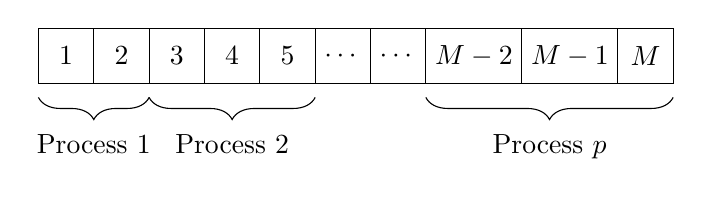
\begin{tikzpicture}[
%  -{Stealth[length = 2.5pt]},
       start chain = going right,
     node distance = 0pt,
MyStyle/.style={draw, minimum width=2em, minimum height=2em, 
                outer sep=0pt, on chain},
  ]
\node [MyStyle] (1) {$1$};
\node [MyStyle] (2) {$2$};
\node [MyStyle] (3) {$3$};
\node [MyStyle] (4) {$4$};
\node [MyStyle] (5) {$5$};
\node [MyStyle] (6) {$\cdots$};
\node [MyStyle] (7) {$\cdots$};
\node [MyStyle] (8) {$M-2$};
\node [MyStyle] (9) {$M-1$};
\node [MyStyle] (10) {$M$};

\draw[decorate,decoration={brace, amplitude=8pt, raise=5pt, mirror}]
  (1.south west) to node[black,midway,below= 15pt] {Process 1} (2.south east);

\draw[decorate,decoration={brace, amplitude=8pt, raise=5pt, mirror}]
  (3.south west) to node[black,midway,below= 15pt] {Process 2} (5.south east);
  
\draw[decorate,decoration={brace, amplitude=8pt, raise=5pt, mirror}]
  (8.south west) to node[black,midway,below= 15pt] {Process $p$} (10.south east);
\end{tikzpicture}
\caption{An illustration of how the work of evaluating $M$ independent features can be distributed among $p$ processes.}
\label{body:parallelism_diag}
\end{figure}


For example, in the computation of the $t$-statistic of each feature, 10 processes were used to distribute the computational work. A pool of worker processes was created with the \texttt{Pool} class in the \texttt{multiprocessing} package in Python. Next, a \texttt{partition\_list} method was written to divide the search space into groups of features for the processes to work on. The \texttt{Pool.map} method was then used. This maps a method - in this case, the computation of the $t$-statistic - on each of the partitions. The result is an improvement in runtime, from 263 seconds to 94 seconds.

As far as possible, this idea was extended to the other methods, where it is possible to conveniently divide the search space into independent segments. For example, RFS (see algorithm \ref{RFSAlgo}) can be parallelised in both of the \texttt{for} loops.

\section{High performance computing} \label{hpc}

Most of the computation for this project was performed using the High Performance Computing (HPC) cluster at Imperial College \cite{RefWorks:218}. In particular, the \texttt{cx1} general purpose computer cluster was used and the \texttt{PBSPro} queueing system was used to manage the jobs submitted by users. The \texttt{cx1} system provided a convenient and highly efficient means to perform computations that required a long time or a large memory demand.

Users of the HPC cluster are provided with three directories: \texttt{\$WORK}, \texttt{\$HOME} and \texttt{\$TMPDIR}. \texttt{\$WORK} and \texttt{\$HOME} are directories that allow users to store data and files. On the other hand, \texttt{\$TMPDIR} is a directory for submitting jobs to the PBS system.

A job is submitted to the system by submitting a job script that first specifies the walltime and memory that the job expects. The job script then lists bash commands, which, for example, copies files and runs Python programs. Most of the Python programs in this project write numerical results to a text file. These text files are then copied to the \texttt{\$WORK} directory, from which we can copy to our local machines.

Furthermore, the cluster allowed \textit{serial jobs} to be conducted. That is, jobs that require multiple executions can be submitted and the program will be run for a specified number of times automatically. This feature was especially convenient for the execution of the GAs. 10 runs of the GA were performed for each of the selection strategies (roulette wheel and tournament), and serial execution made this task much easier.


\chapter{Experimental results and evaluation}
\label{evaluation}

\section{$t$-test}
Plots were obtained from $t$-test using different experimental settings:
\begin{itemize}
  \item Sample $k$ in broad intervals to investigate the general trend of $t$-test (Figure \ref{body:t_test:fig:range}).
  \item Sample $k\in [10,2000)$ with step size of 10 (Figure \ref{body:t_test:fig}).
  \item Magnified view of Figure \ref{body:t_test:fig}, where $k \in [10,2000)$ (Figure \ref{body:t_test:fig_zoom}).
\end{itemize}
where $k$ is the number of features selected.

When plotting such graphs, we also investigate if the selected subset of features $S$ causes the SVM to suffer significant performance degradation as compared to using all the features. To this end, a horizontal dotted line can be found in the graphs. This dotted line represents a \textit{threshold}, which is the linear SVM's performance when using all of the features.

\subsection{Broad intervals of $k$}
The first experiment broadly samples $k$ from a range of values. The values of $k$ and the corresponding cross validation (CV) scores are shown in Table \ref{t_test:table:range}. For this table of values, we sampled $k$ from 1 to 420374 (the full set of features). 

\begin{table}[h!]
\centering
\begin{tabular}{|c||c|c|c|c|c|c|c|}
\hline
$k$      & 1        & 5        & 10       & 20       & 50       & 80       & 100      \\ \hline
CV score & 0.7001   & 0.837137 & 0.848937 & 0.863068 & 0.846479 & 0.861801 & 0.867704 \\ \hline \hline
$k$      & 250      & 500      & 750      & 1000     & 2000     & 5000     & 8000     \\ \hline
CV score & 0.882004 & 0.893754 & 0.907942 & 0.907921 & 0.93035  & 0.943376 & 0.949279 \\ \hline \hline
$k$      & 10000    & \textbf{15000}    & 20000    & 40000    & 80000    & 100000   & 150000   \\ \hline
CV score & 0.950441 & \textbf{0.950448} & 0.946877 & 0.949258 & 0.946891 & 0.942171 & 0.939783 \\ \hline \hline
$k$      & 250000   & 300000   & 400000   & 420374   &          &          &          \\ \hline
CV score & 0.938628 & 0.937444 & 0.932703 & 0.92916  &          &          &          \\ \hline
\end{tabular}
\caption{Table of CV scores with the number of features ($k$) selected for classification. The maximum CV score and its corresponding $k$ are highlighted in bold.}
\label{t_test:table:range}
\end{table}

As mentioned in section \ref{t-test}, the $t$-test allows us to generate a list of $p$-values and we then sort the $p$-values in ascending order. For each $k$, we will select the top $k$ features from the sorted list, fit an SVM with the $k$ features, and obtain CV scores. For example, when $k=500$, we will select the top 500 features in the sorted list.

From Figure \ref{body:t_test:fig:range}, we notice that the CV score peaks at around $k=15000$ with a score of 0.950448, and after this value of $k$, the CV score exhibits a decreasing trend. Evidently, due to the coarse granularity of $k$ that we have sampled, this method might have missed out on some local maxima after $k=15000$. However, because the time required to fit an SVM and obtain CV scores increases with the number of features, it is perhaps sufficient to obtain a broad, general trend of $t$-test.

\subsection{Specific range of $k$}
If we are interested in a specific range of $k$, we can easily plot a similar graph and sample $k$ with smaller step sizes. This is shown in Figure \ref{body:t_test:fig}, where $k$ ranges from 10 to 2000 with a step size of 10. That is, we have $k=10,20, \dots, 2000$. In this graph, we can see a similar trend, where the CV score increases with the number of features. The CV score peaks at around $k=1500$.

To investigate where exactly the peak lies, we can zero in on a specific range of $k$ and sample $k$ with an even smaller step size. In Figure \ref{body:t_test:fig_zoom}, $k$ ranges from 1500 to 1600 with step size of 1. The peak is precisely $k=1589$, where the corresponding CV score is around 0.932738. We can see that even with a small set of features, we can perform better than the threshold.

%This shows that most of the features are actually not needed for good accuracy.

%%%%%%%%%% TABLE AND FIGURES %%%%%%%%%%%%%

\begin{figure}
\centering
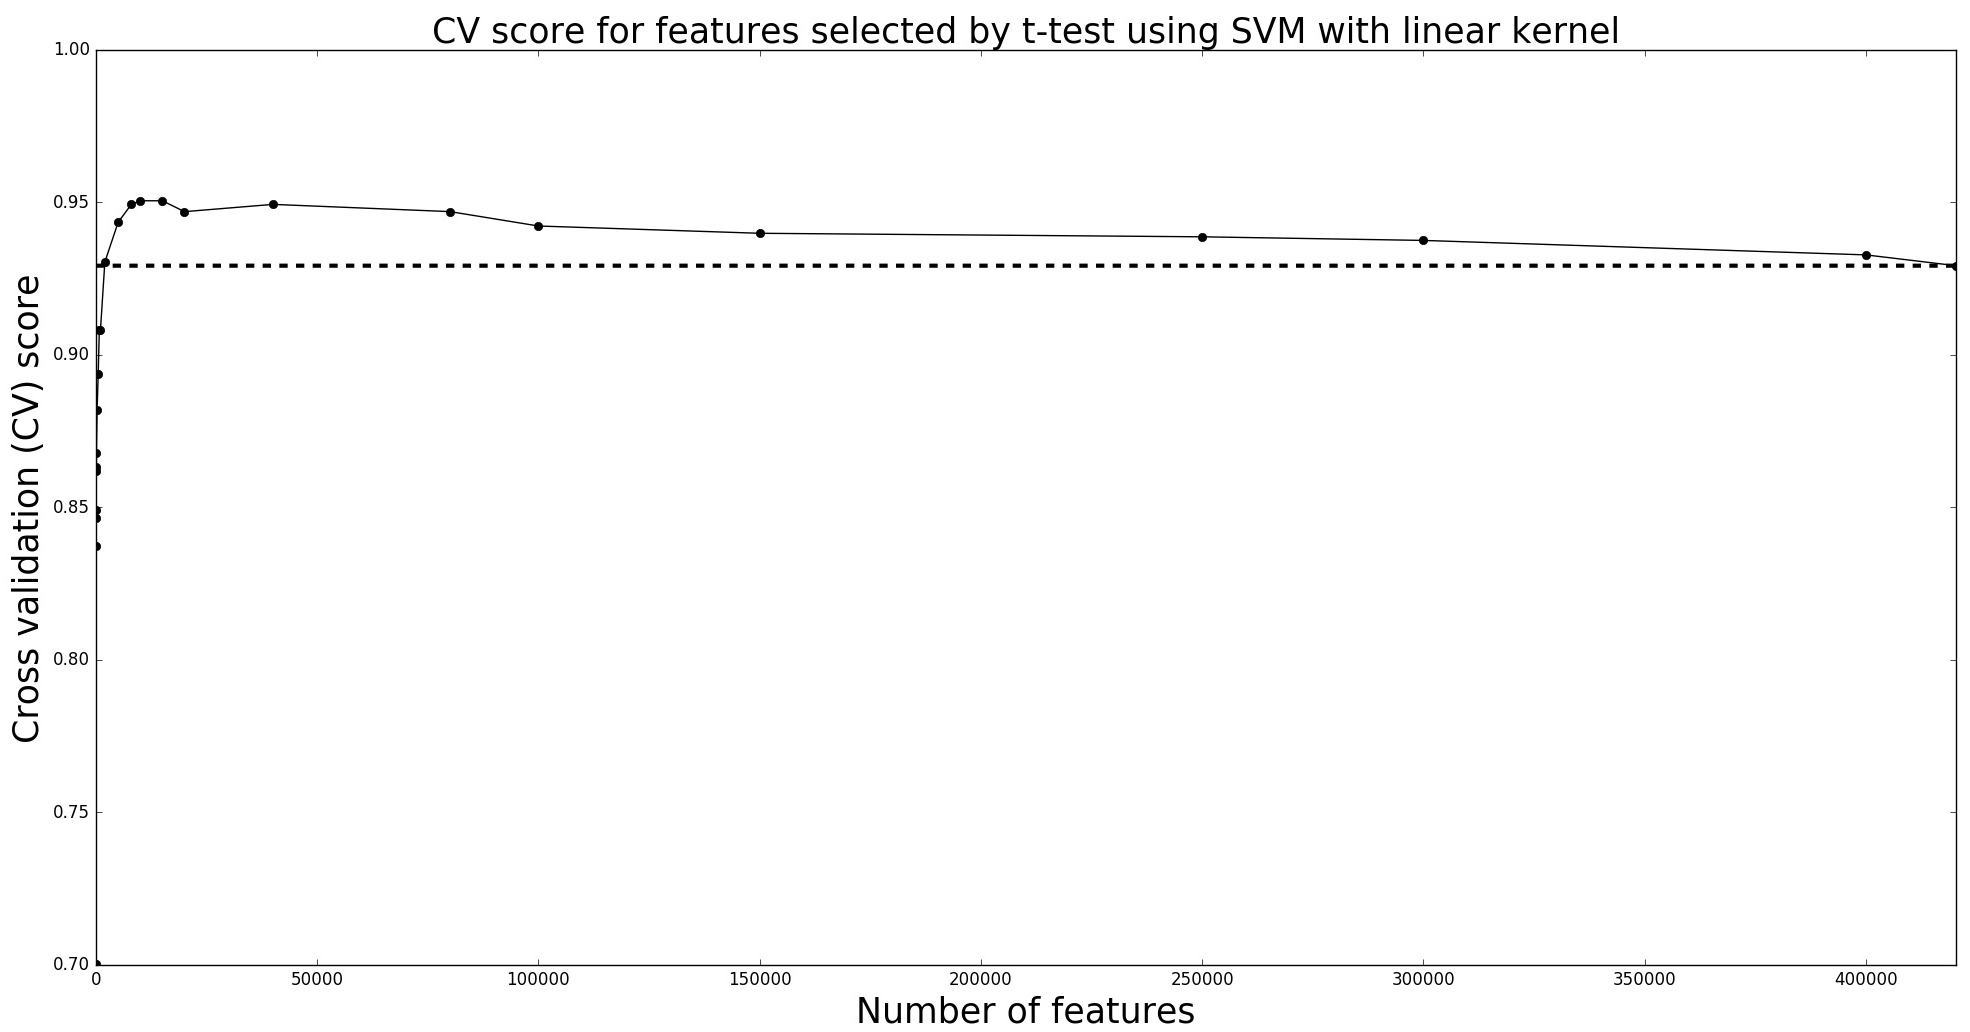
\includegraphics[width=\textwidth]{images/t_test_range.jpeg}
\caption{Plot of CV score against number of features, when an SVM with a linear kernel is fitted with the selected number of features.}
\label{body:t_test:fig:range}
\end{figure}

\begin{figure}
\centering
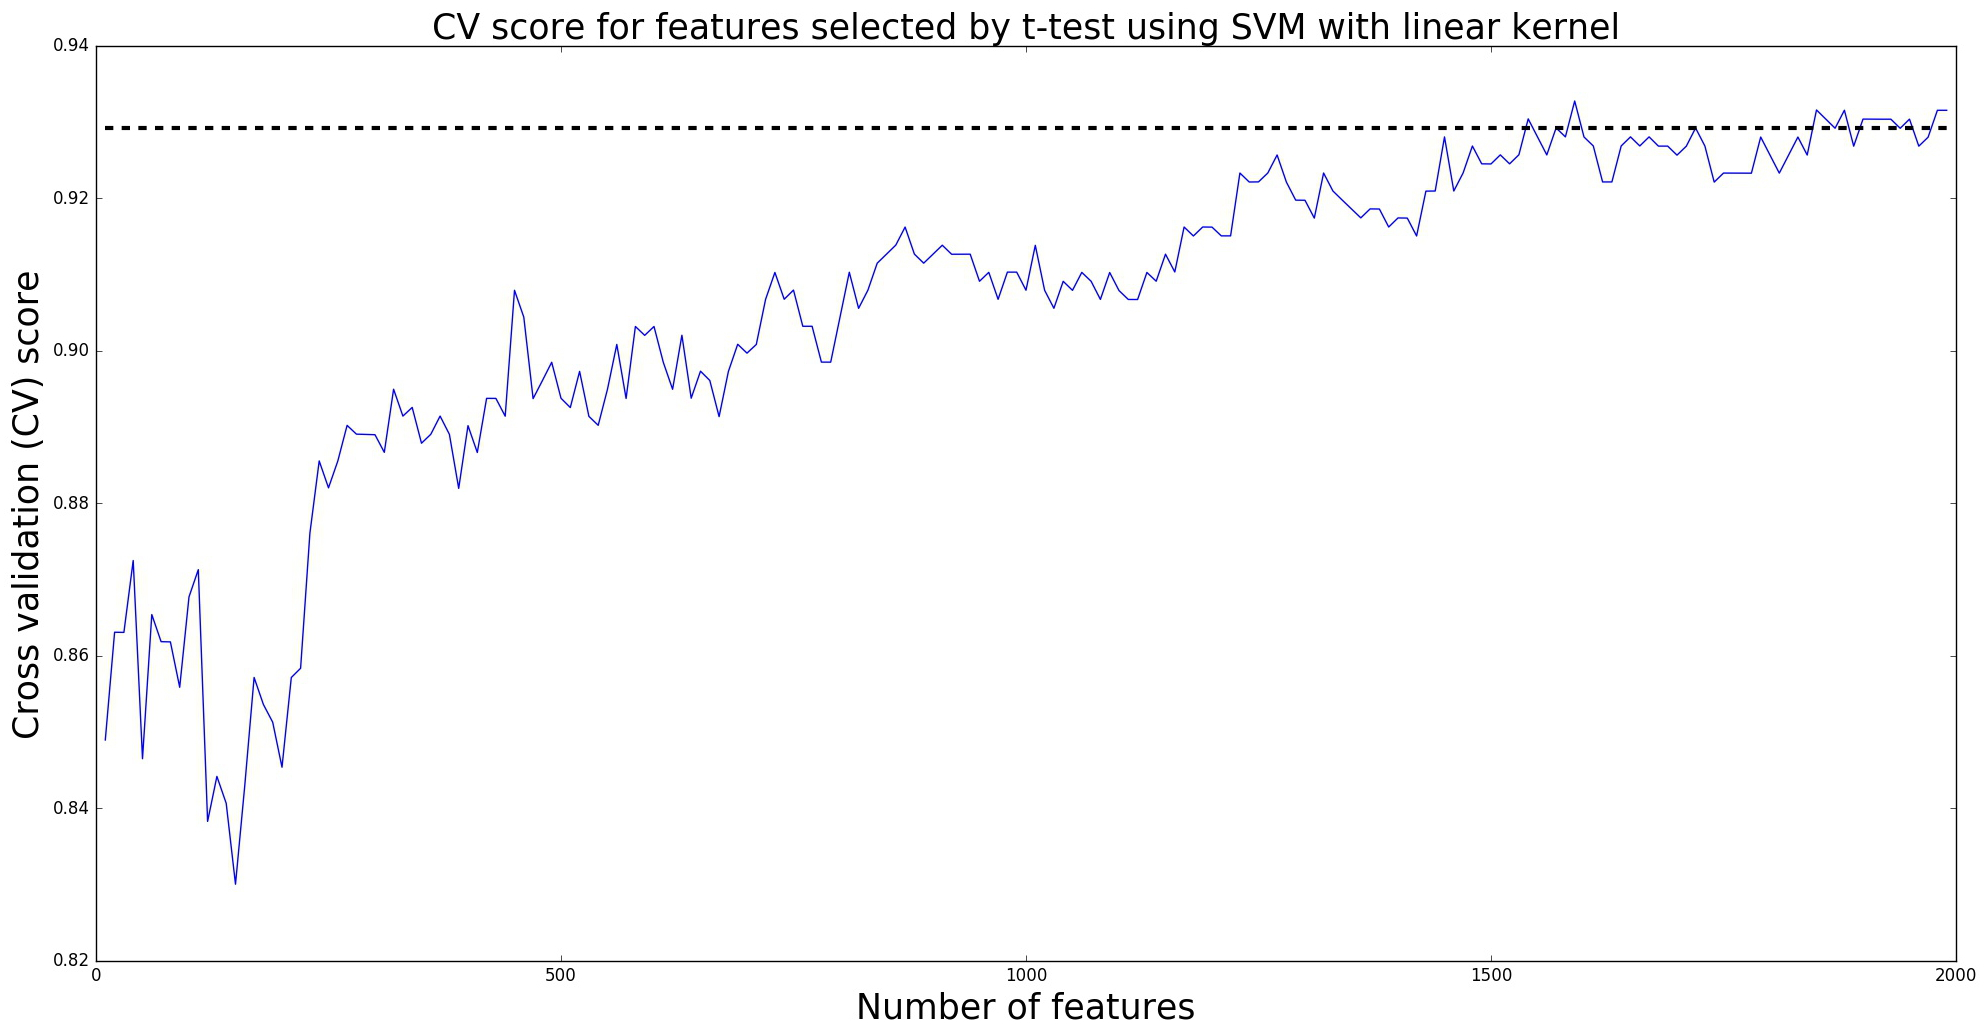
\includegraphics[width=\textwidth]{images/t_test_2000_uneq_var1.jpeg}
\caption{Plot of cross validation score against number of features, when an SVM with a linear kernel is fitted with the selected number of features, $k \in [10, 2000)$, with step size of 10.}
\label{body:t_test:fig}
\end{figure}

\begin{figure}
\centering
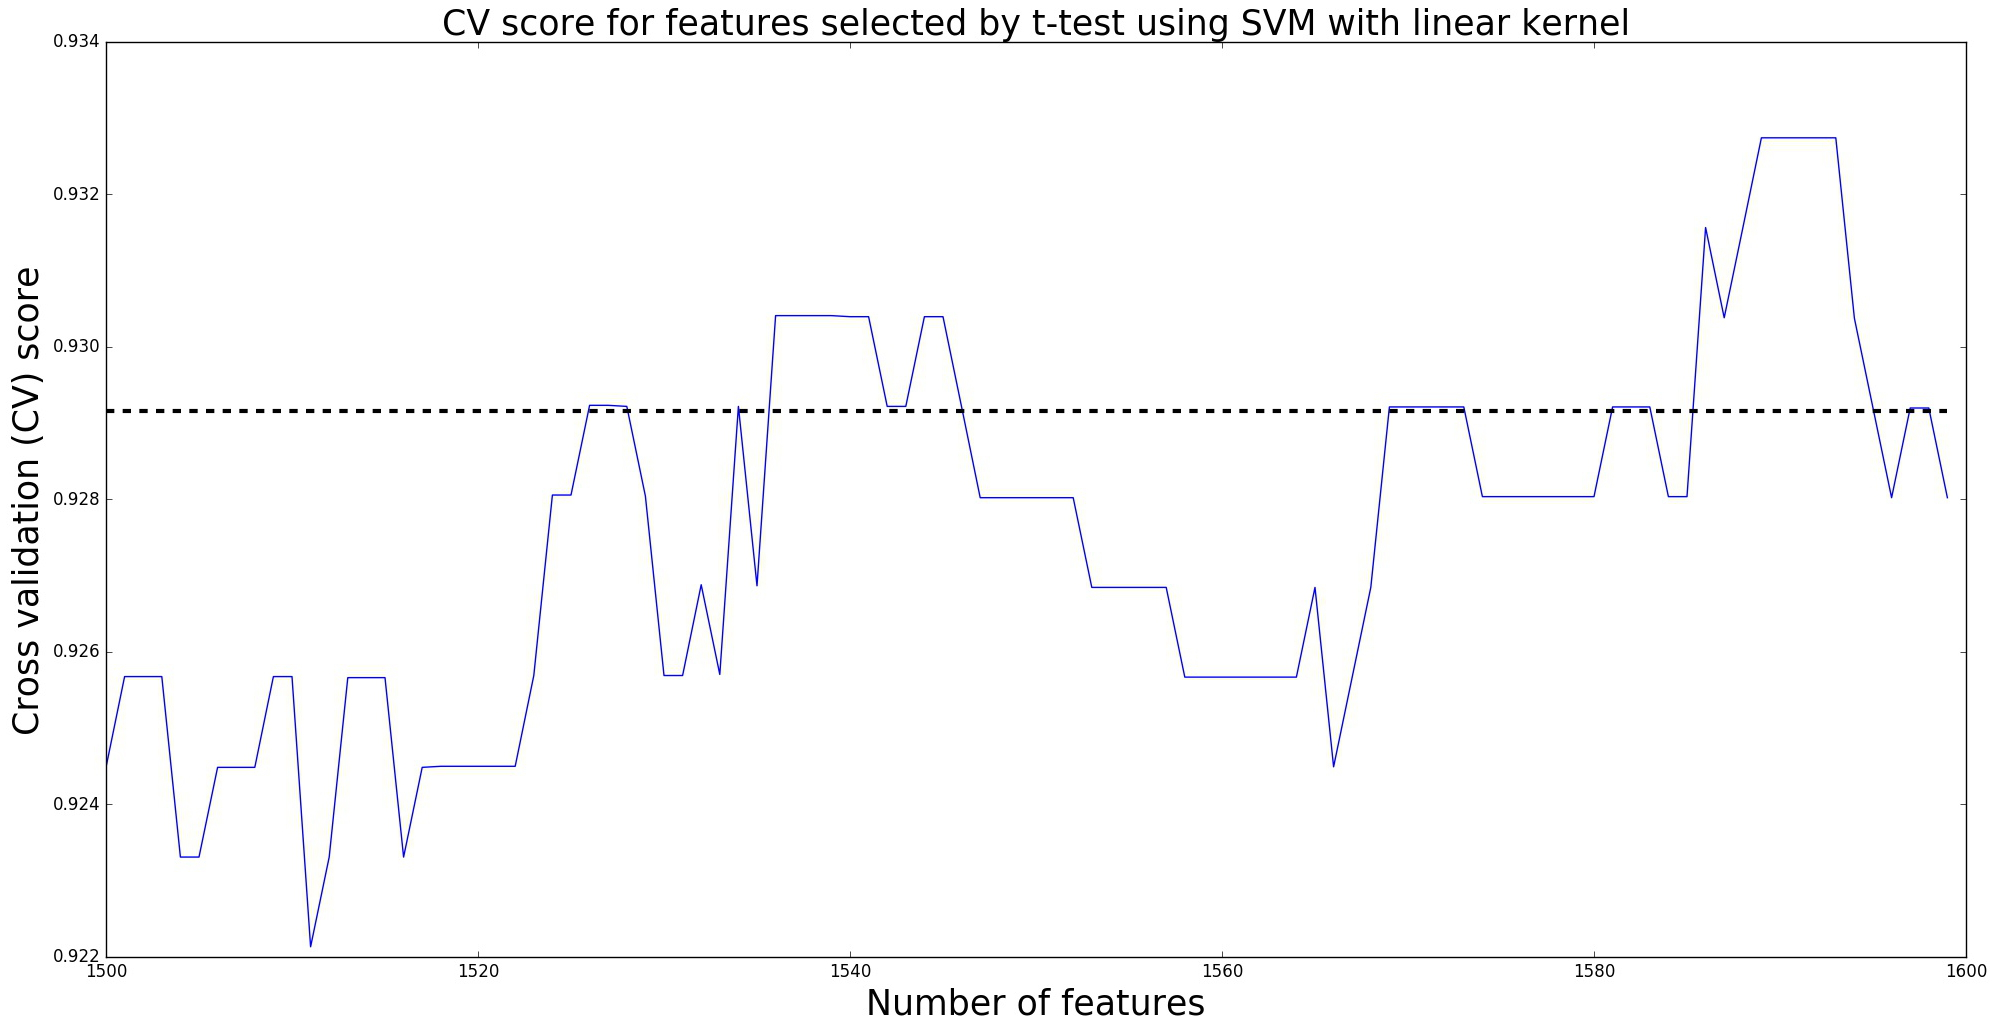
\includegraphics[width=\textwidth]{images/t_test_2000_uneq_var_zoom.jpeg}
\caption{A magnified view of Figure \ref{body:t_test:fig}. The peak is at $k=1589$.}
\label{body:t_test:fig_zoom}
\end{figure}

\subsection{Lazy variation of SFS}
Here, we investigate the lazy variation of SFS, as discussed in section \ref{body:sfs:lazy}. Instead of $p$-values, we sort the features according to their individual CV scores. We then obtain Figure \ref{body:lazy_sfs:graph}. 

\begin{figure}
\centering
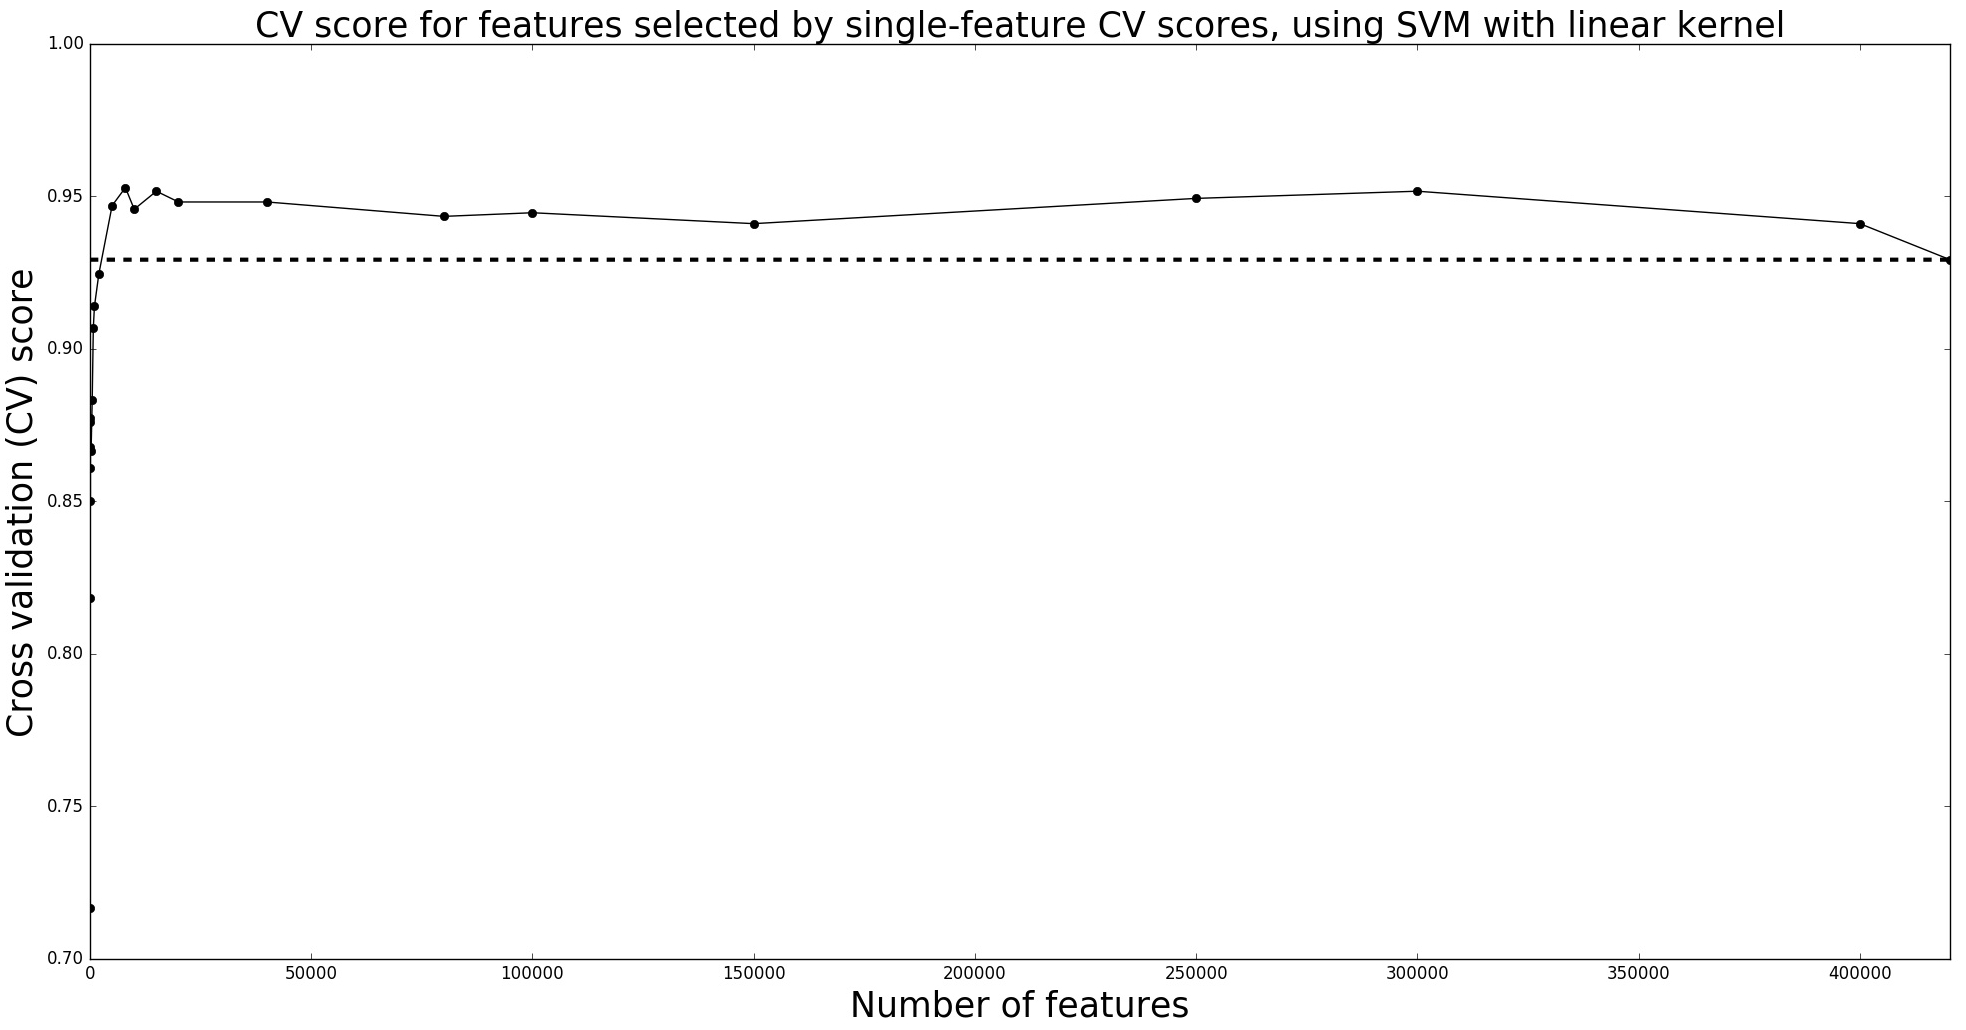
\includegraphics[width=\textwidth]{images/lazy_sfs_range.jpeg}
\caption{A graph of CV scores against number of features using a lazy variation of Sequential Forward Selection.}
\label{body:lazy_sfs:graph}
\end{figure}

We can see from the graph that at first, there is a similar trend to that in $t$-test in Figure \ref{body:t_test:fig:range}: the CV score increases at a very fast rate and peaks at $k=8000$ with CV score 0.952794.  The CV score then decreases with more features. However, unlike the graph in Figure \ref{body:t_test:fig:range}, the CV score peaks again slightly at around $k=300000$. We can investigate this slight peak by plotting another graph shown in Figure \ref{body:lazy_sfs_smaller_range:graph}, focusing on features between 250000 and 320000 with a step size of 1000. The maximum CV score in this range was 0.955161 with $k=310000$.

\subsection{Comparing $t$-test and lazy SFS}
Using lazy SFS, the subset with 310000 features performs slightly better than that with 8000 features, but the former has about 40 times as many features as the latter. In this case, it might be sensible to compromise 0.3\% of classification accuracy for about 300000 lesser features, as selecting only 8000 features for classification will impose much smaller computational and time constraints. Besides, it will be easier to make biological conclusions. This reflects the trade-offs faced in feature selection. We can also compare the lazy SFS and $t$-test clearly when we plot the two graphs in the same diagram in Figure \ref{body:t_test_and_lazy_sfs:graph}.

Moreover, from the graph in Figure \ref{body:t_test_and_lazy_sfs:graph}, we can see that both methods have similar performance when $k$ is relatively small (i.e. $k<150000$). However, beyond this value of $k$, the lazy SFS method seems to outperform the $t$-test method, although the difference in CV score is not significant (about 0.01).

\begin{figure}
\centering
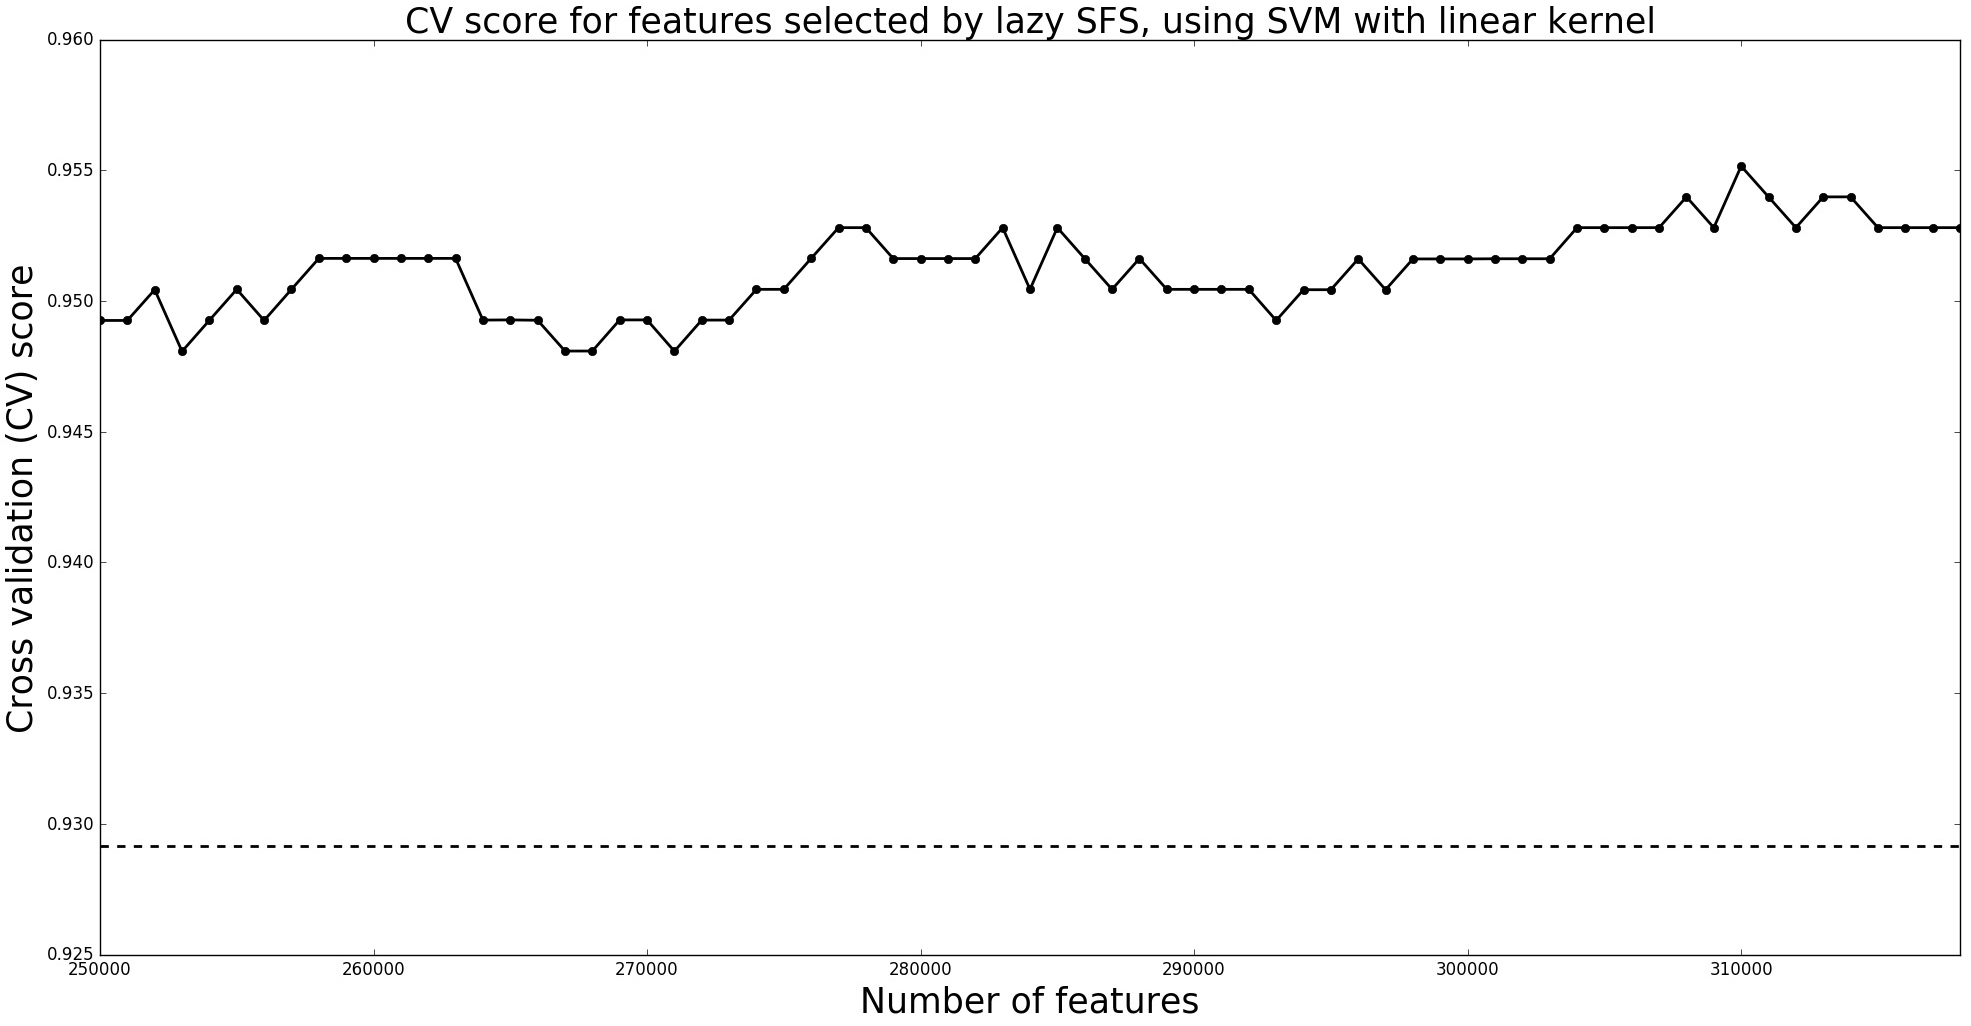
\includegraphics[width=\textwidth]{images/lazy_sfs_smaller_range.jpeg}
\caption{A ``magnified'' graph of CV scores against number of features using lazy SFS, focusing on the slight peak at around $k=300000$.}
\label{body:lazy_sfs_smaller_range:graph}
\end{figure}

\begin{figure}
\centering
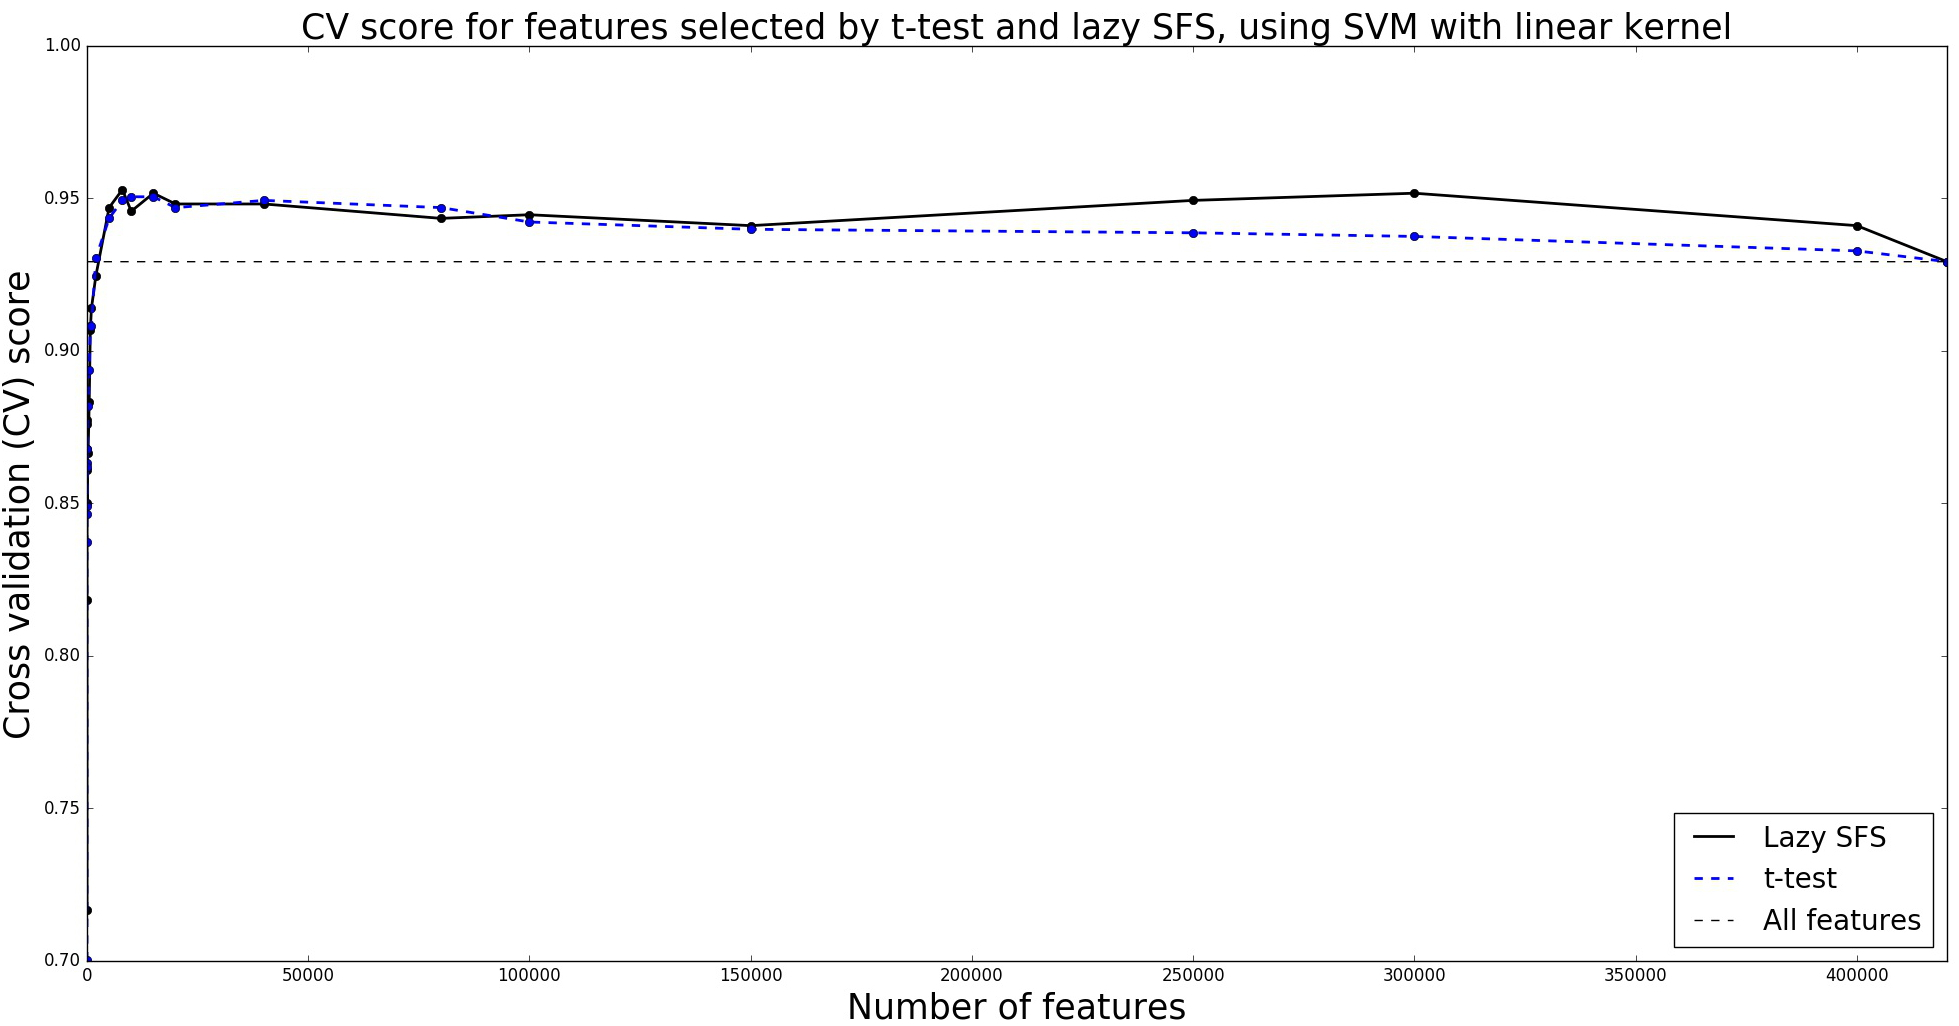
\includegraphics[width=\textwidth]{images/t_test_and_lazy_sfs.jpeg}
\caption{A graph of CV scores against number of features using both $t$-test and lazy SFS.}
\label{body:t_test_and_lazy_sfs:graph}
\end{figure}

Similarly to the discussion for the $t$-test method, the lazy SFS method only considers each feature singly, and does not take into account any form of redundancy; features that perform well individually might be redundant with respect to other features. Furthermore, features that do not perform well individually might perform well with other features, as discussed in \cite{RefWorks:140}.

%It is also interesting to note that the $t$-test gives a maximum CV score of 0.950448 with $k=15000$, while using the lazy SFS method (ignoring the peak at $k=310000$), we get a maximum CV score of 0.952794 with $k=8000$. Evidently, the lazy SFS method can produce a smaller subset that performs slightly better than the one selected by the $t$-test.

Overall, both the $t$-test and the lazy SFS methods produce subsets with good performance relative to the threshold, but we also note that both methods do not take redundancy into account.


\section{Recursive Feature Elimination} \label{eval:rfe}

\subsection{Varying step size}
As mentioned in section \ref{body:rfe}, the RFE algorithm removes \texttt{step} number of features which have the lowest weights in each iteration. In implementing RFE, the step size was made to vary according to the number of features that we desire. This variation is summarised in Table \ref{rfe_results_table}. For example, suppose we wanted to select only $k=5$ features. It will not be sensible to set the step size to a small number like 1, because the algorithm starts with the full set of features. Setting step size to 1 means that the algorithm will remove 1 feature at a time and thus the algorithm will take a very long time to terminate.

%Since it takes a long time to perform cross validation with many features, it will take a very long for the algorithm to terminate.

We then obtain CV scores based on the features selected by the algorithm. The CV scores can also be found in Table \ref{rfe_results_table}.

Next, we plot a graph of how the CV scores vary with the number of features selected. This graph can be found in Figure \ref{body:rfe:graph}.

%We also plot the CV scores against the number of features that were specified. This graph can be found in Figure \ref{body:rfe:graph_1}.

\subsection{Performance of RFE}
From Figure \ref{body:rfe:graph}, we can see that there is an overall increasing trend in the CV scores. However, all the scores fall below the threshold. Evidently, using RFE to select features does not seem to benefit the feature selection method. We can compare this result to the $t$-test experiments performed earlier. We notice that using the $t$-test seems to produce better results than RFE. Besides, $t$-test is also computationally much less expensive than RFE.

Regardless, we also need to take into account how the \texttt{step} parameter works in the RFE method. At each iteration, the algorithm tries to fit an SVM on the features. Suppose it is considering $F$ features, and the step size is $f$. It will remove $f$ features that have the lowest weights until the number of features needed is achieved. Thus, the step size $f$ here is important. From Table \ref{rfe_results_table}, we can see that the step sizes assigned to the algorithm are relatively large. For example, if we want only 10 features, the algorithm removes 10000 features at a time, which is a lot of features. This was done to allow the algorithm to terminate within a reasonable amount of time. Thus, this coarse step size might miss out on certain local optima which might be a cause of the trend we observe in RFE.

We also note that RFE suffers from the same \textit{nesting effect} that Sequential Forward Selection and Sequential Backward Selection both experience, discussed in section \ref{bg:fs:greedy}. That is, once features are eliminated, they are not considered again by the algorithm.

From the above discussion, we can conclude that RFE might not be a good method to select features from our data set in terms of both computational cost and performance.

\begin{table}
\centering
    \begin{tabular}{ | c | c | c | } \hline
    Step size & Num. of features & CV score \\ \hline
    \multirow{9}{*}{10000} & 
  1 & 0.5900  \\
 & 5 & 0.7638   \\
 & 10 & 0.8028  \\
 & 20 & 0.8205  \\
 & 50 & 0.8359 \\
 & 80 & 0.8217 \\
 & 100 & 0.8063 \\
 & 250 & 0.7652 \\
 & 500 & 0.7756 \\ \hline
 
 \multirow{3}{*}{5000} & 
  750 & 0.8276  \\
 & 1000 & 0.8158 \\
 & 2000 & 0.8488 \\ \hline
 
 \multirow{3}{*}{2000} & 
  5000 & 0.8831 \\
 & 8000 & 0.8925 \\
 & 10000 & 0.8972 \\ \hline
 
 \multirow{3}{*}{1500} & 
  15000 & 0.9020 \\
 & 20000 & 0.9043 \\
 & 40000 & 0.9114 \\ \hline
 
 \multirow{6}{*}{1000} & 
  80000 & 0.9091 \\
 & 100000 & 0.9114 \\
 & 150000 & 0.9150 \\
  & 250000 & 0.9126 \\
   & 300000 & 0.9126 \\
    & 400000 & 0.9138 \\ \hline
    \end{tabular}
\caption{Table of step size and corresponding chosen number of features and cross validation scores for Recursive Feature Elimination.}
\label{rfe_results_table}
\end{table}


\begin{figure}
\centering
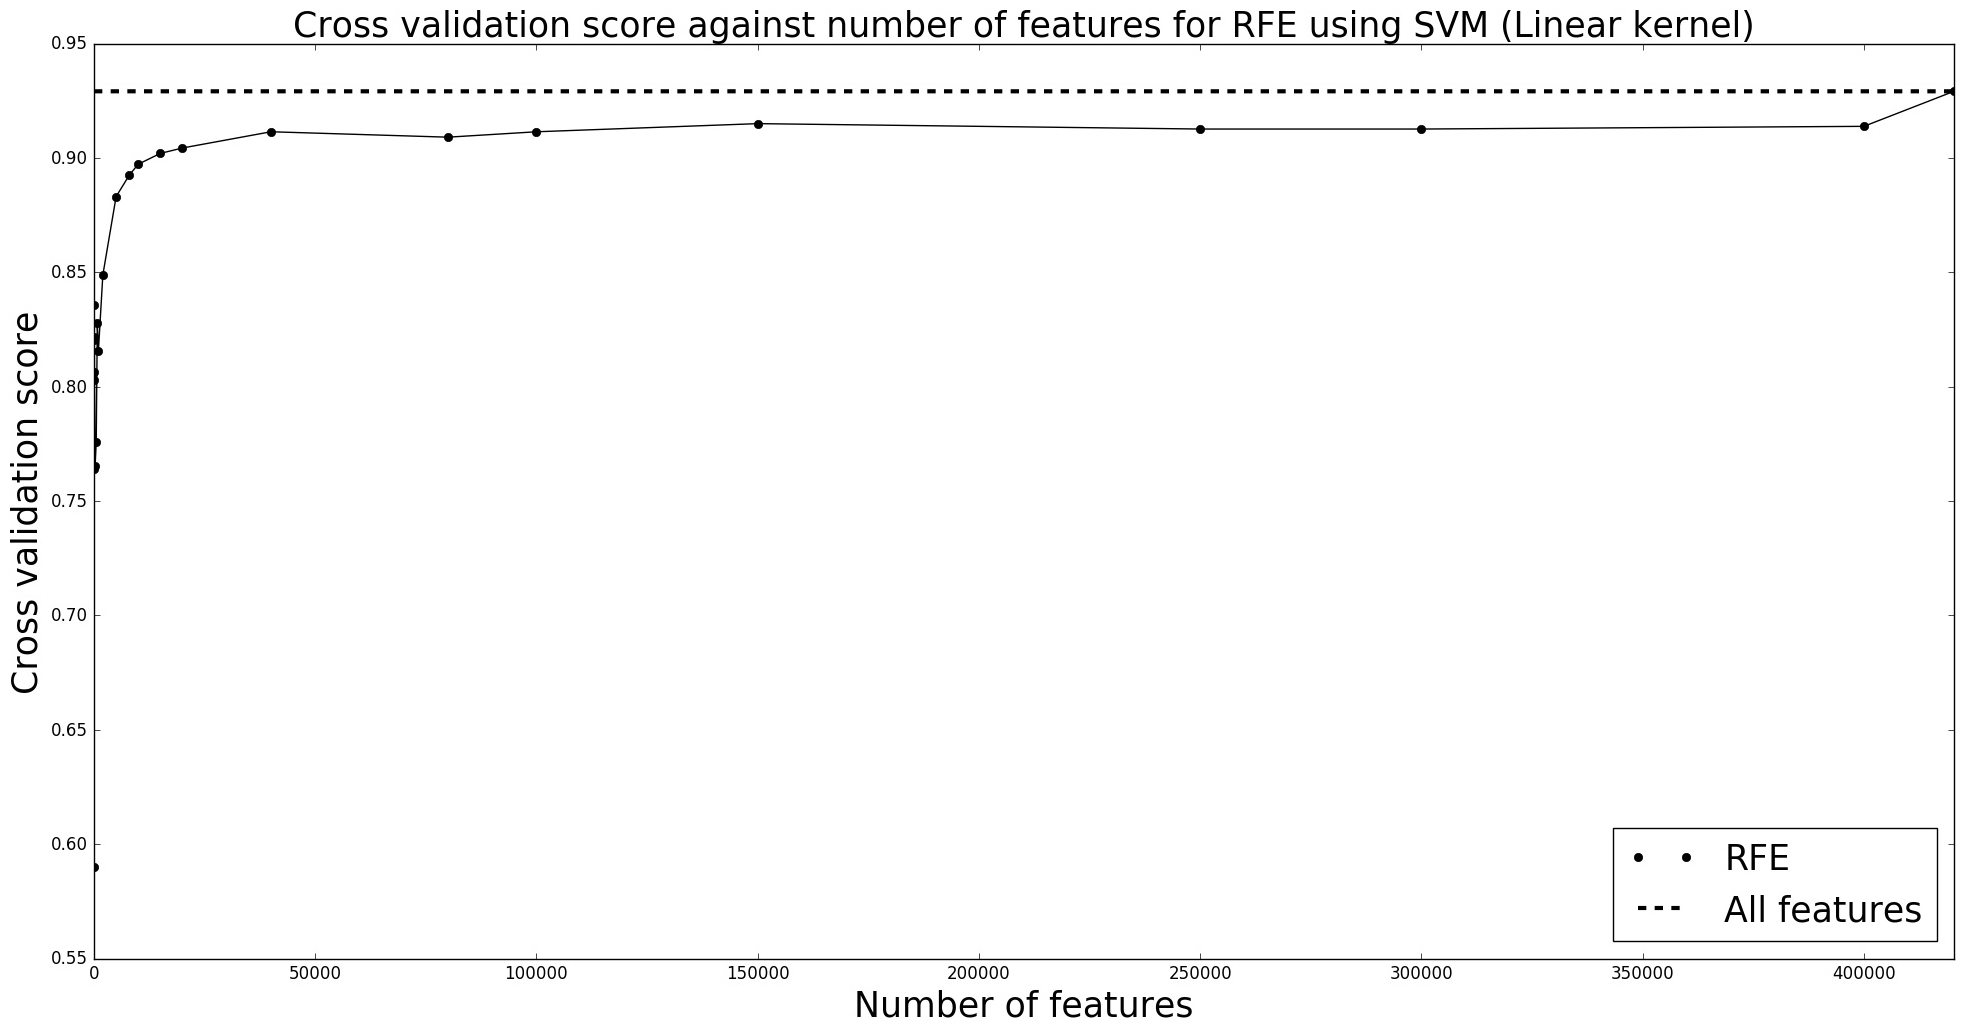
\includegraphics[width=\textwidth]{images/rfe_linear_all.jpeg}
\caption{A graph of CV scores against number of features using both RFE.}
\label{body:rfe:graph}
\end{figure}

\begin{comment}
\begin{figure}
\centering
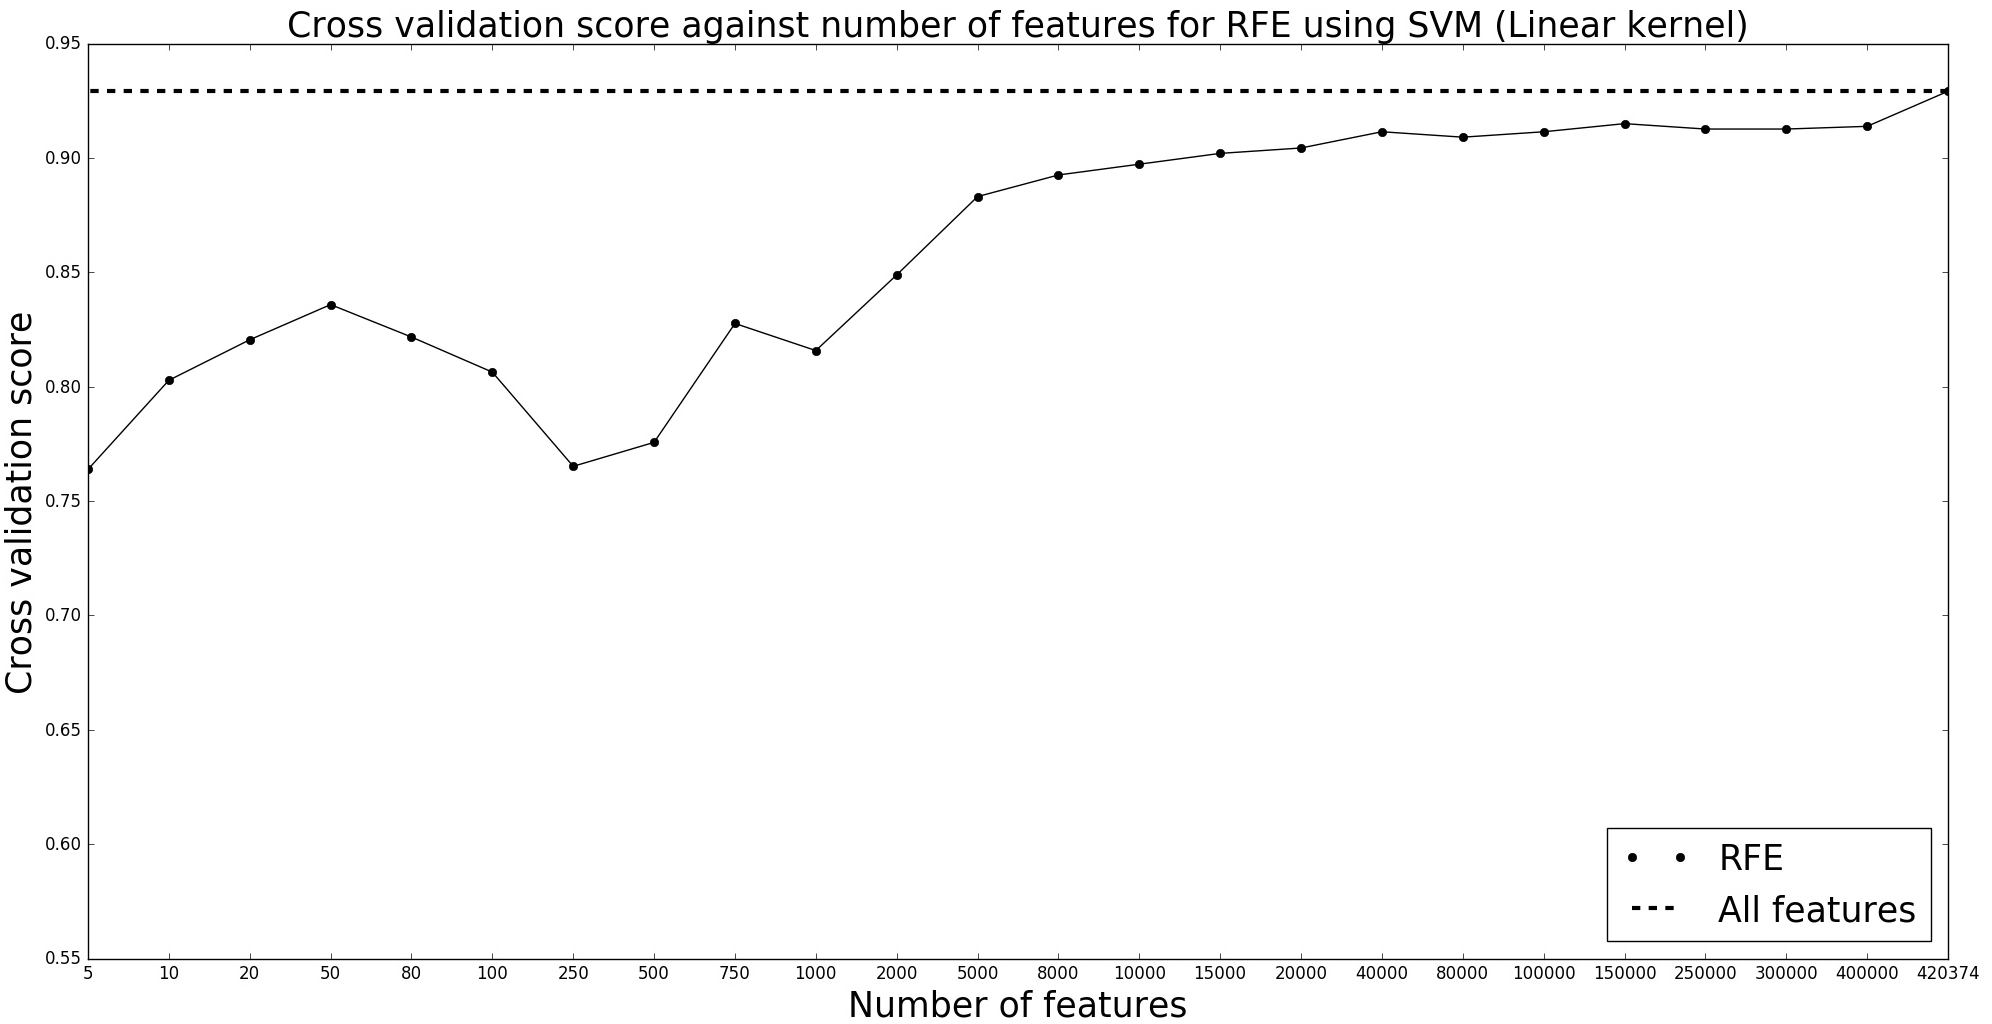
\includegraphics[width=\textwidth]{images/rfe_linear.jpeg}
\caption{A graph of CV scores against number of features using RFE, showing just the trend of the scores.}
\label{body:rfe:graph_1}
\end{figure}
\end{comment}

\section{Restricted Forward Selection}

Due to time constraints, the RFS algorithm was only able to select 800 features, and the corresponding graph can be found in Figure \ref{body:rfs_graph}. We see that across all 800 features, the graph does not exceed the threshold for the linear SVM.

We see that the graph peaks at $k=53$ with a CV score of about 0.89611. After that, the CV score decreases and exhibits a slow increasing trend. However, the CV score does not exceed 0.89611 even with 800 features. We see that since there is an increasing trend in the CV scores, RFS might be able to select a subset that can perform better than the threshold. However, we cannot be absolutely certain about this until we use RFS to select more features. At the time of writing, RFS is being performed with $k=5000$.

\begin{figure}
\centering
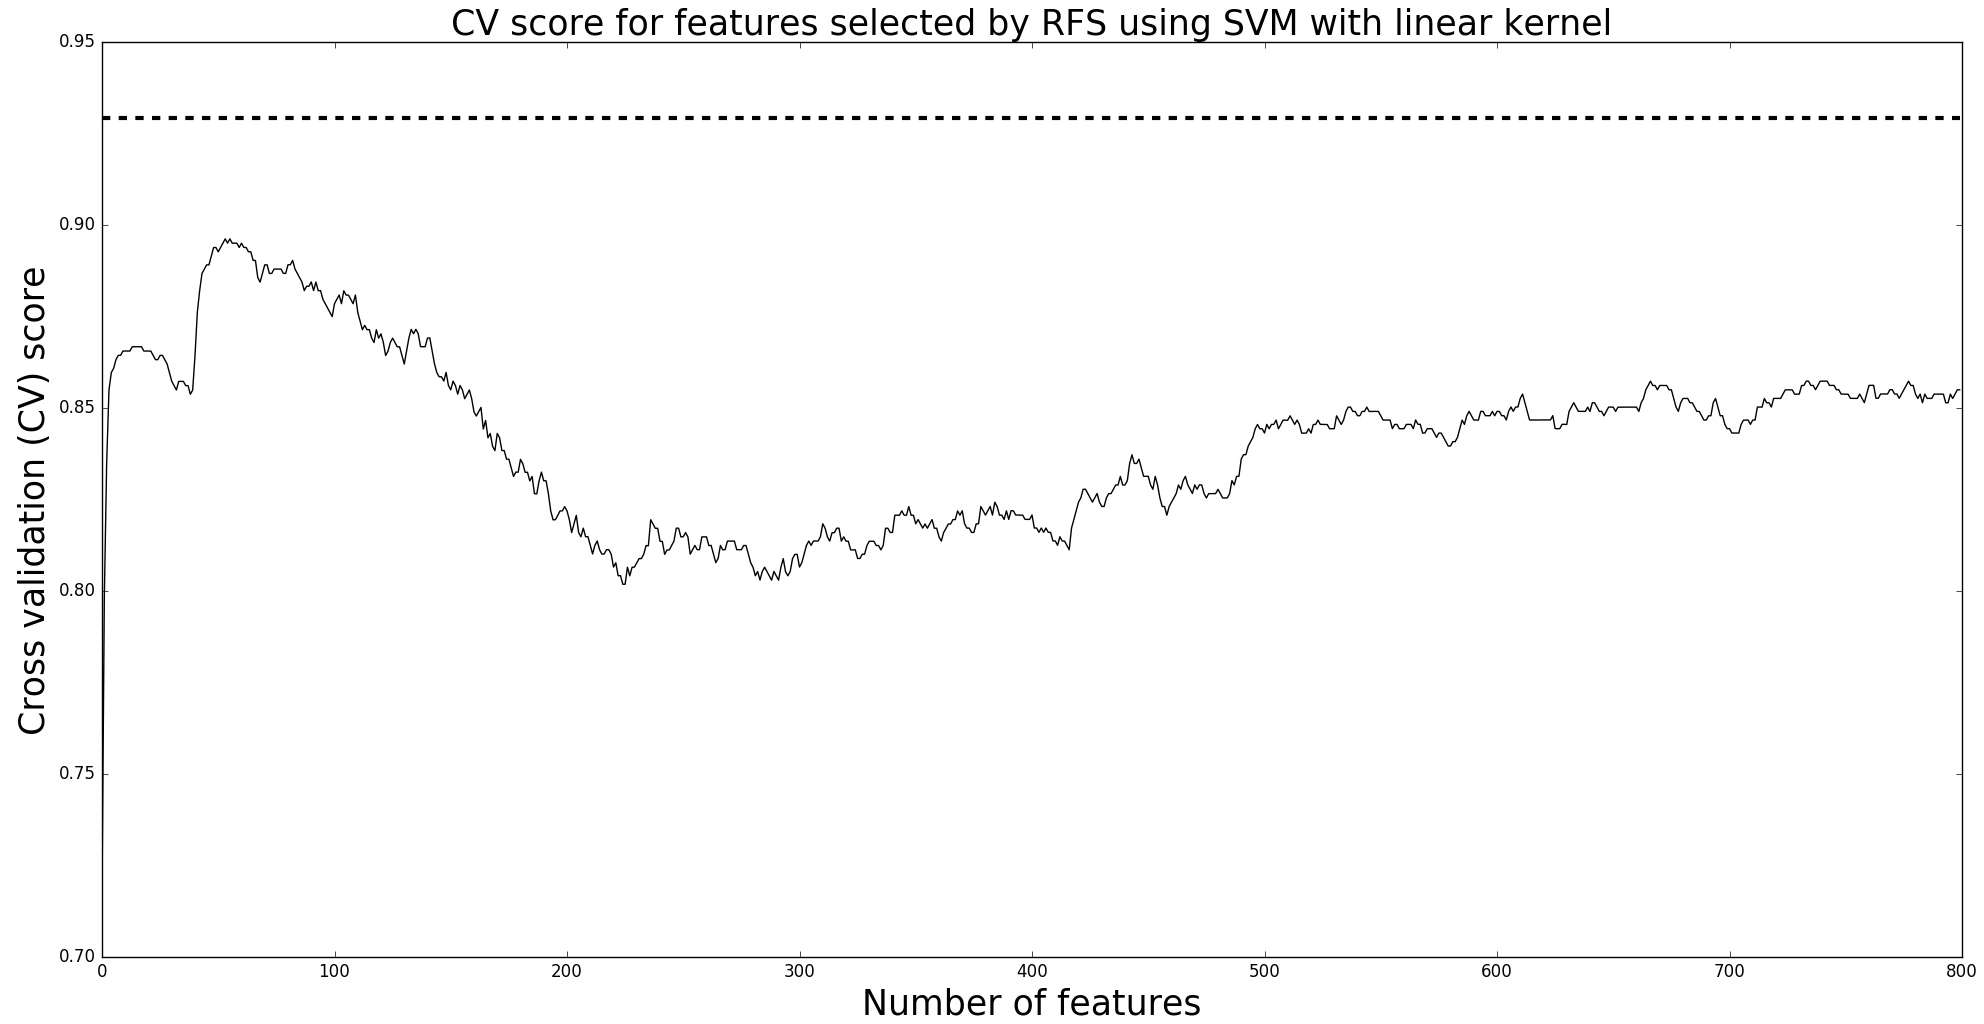
\includegraphics[width=\textwidth]{images/rfs_linear_800.jpeg}
\caption{A graph of CV scores against number of features using Restricted Forward Selection.}
\label{body:rfs_graph}
\end{figure}

\begin{figure}
\centering
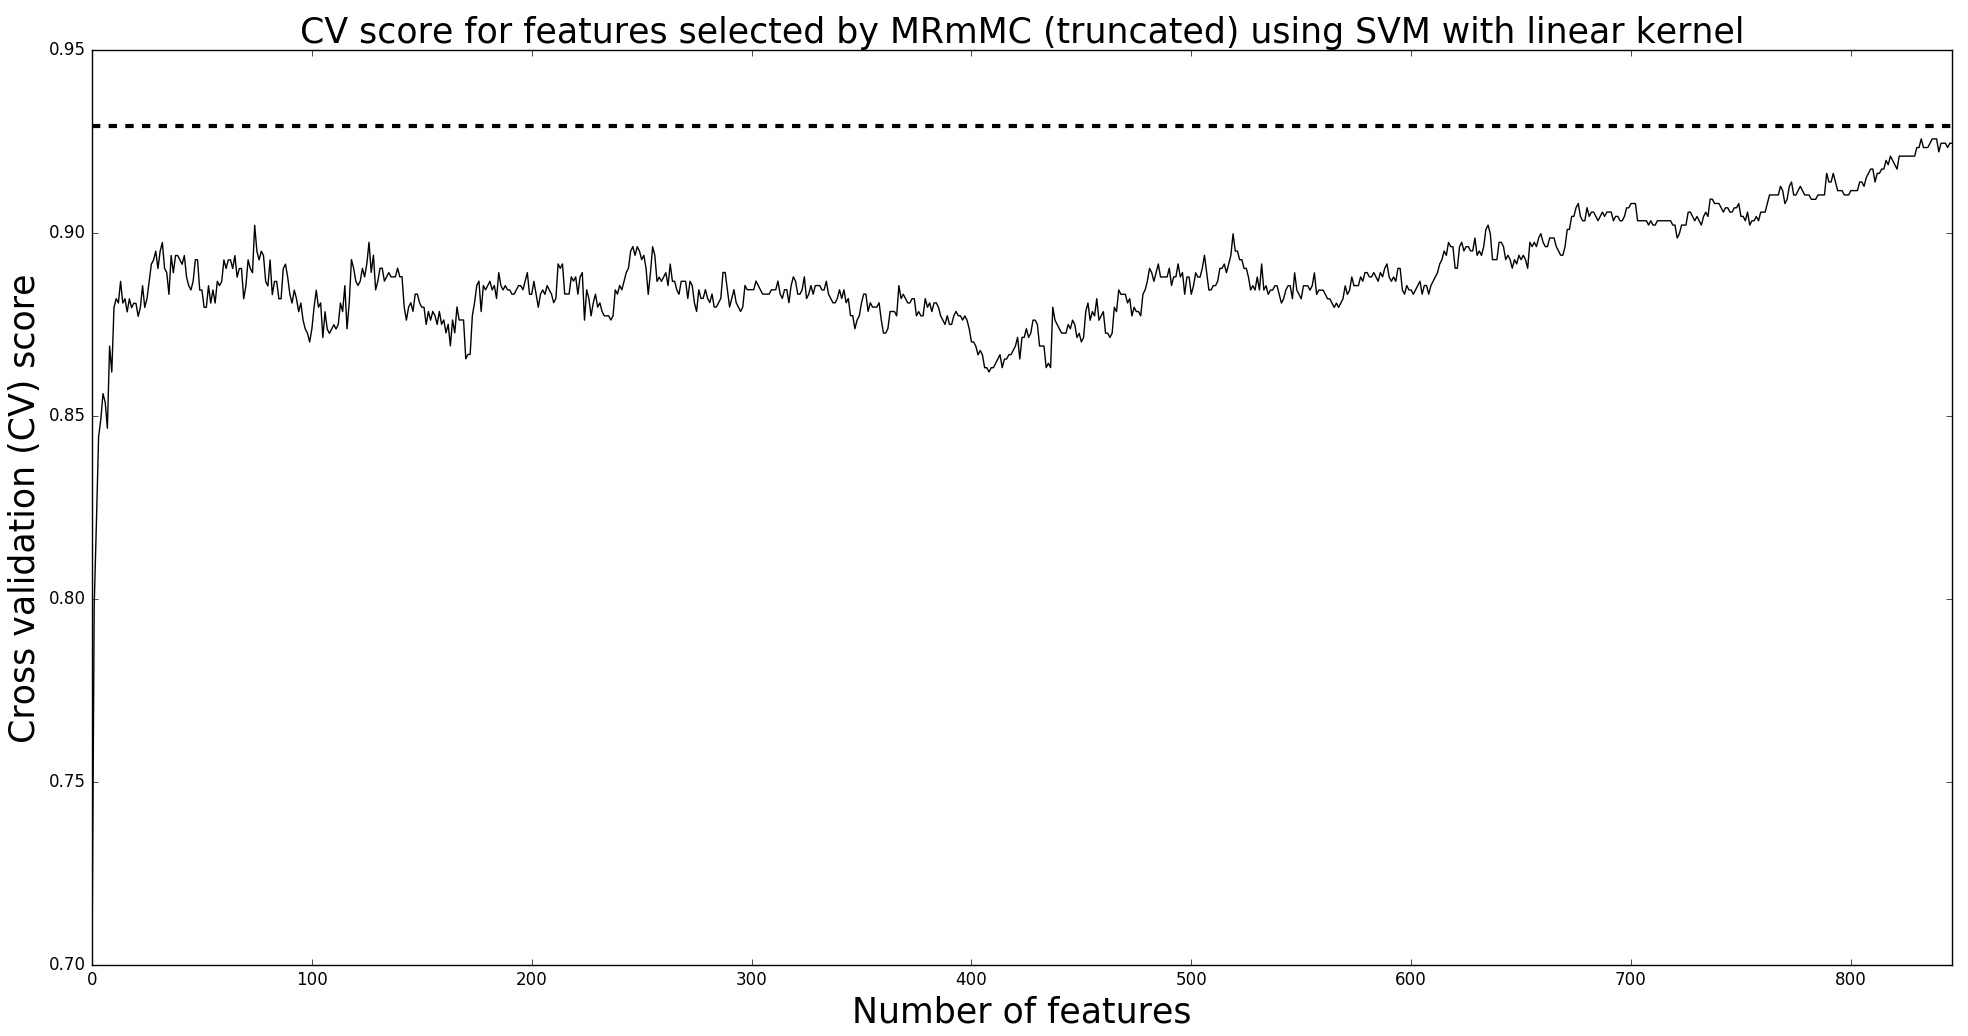
\includegraphics[width=\textwidth]{images/mrmmc_trun_linear_847.jpeg}
\caption{A graph of CV scores against number of features using the truncated version of MRmMC.}
\label{body:mrmmc_trun}
\end{figure}

\begin{figure}
\centering
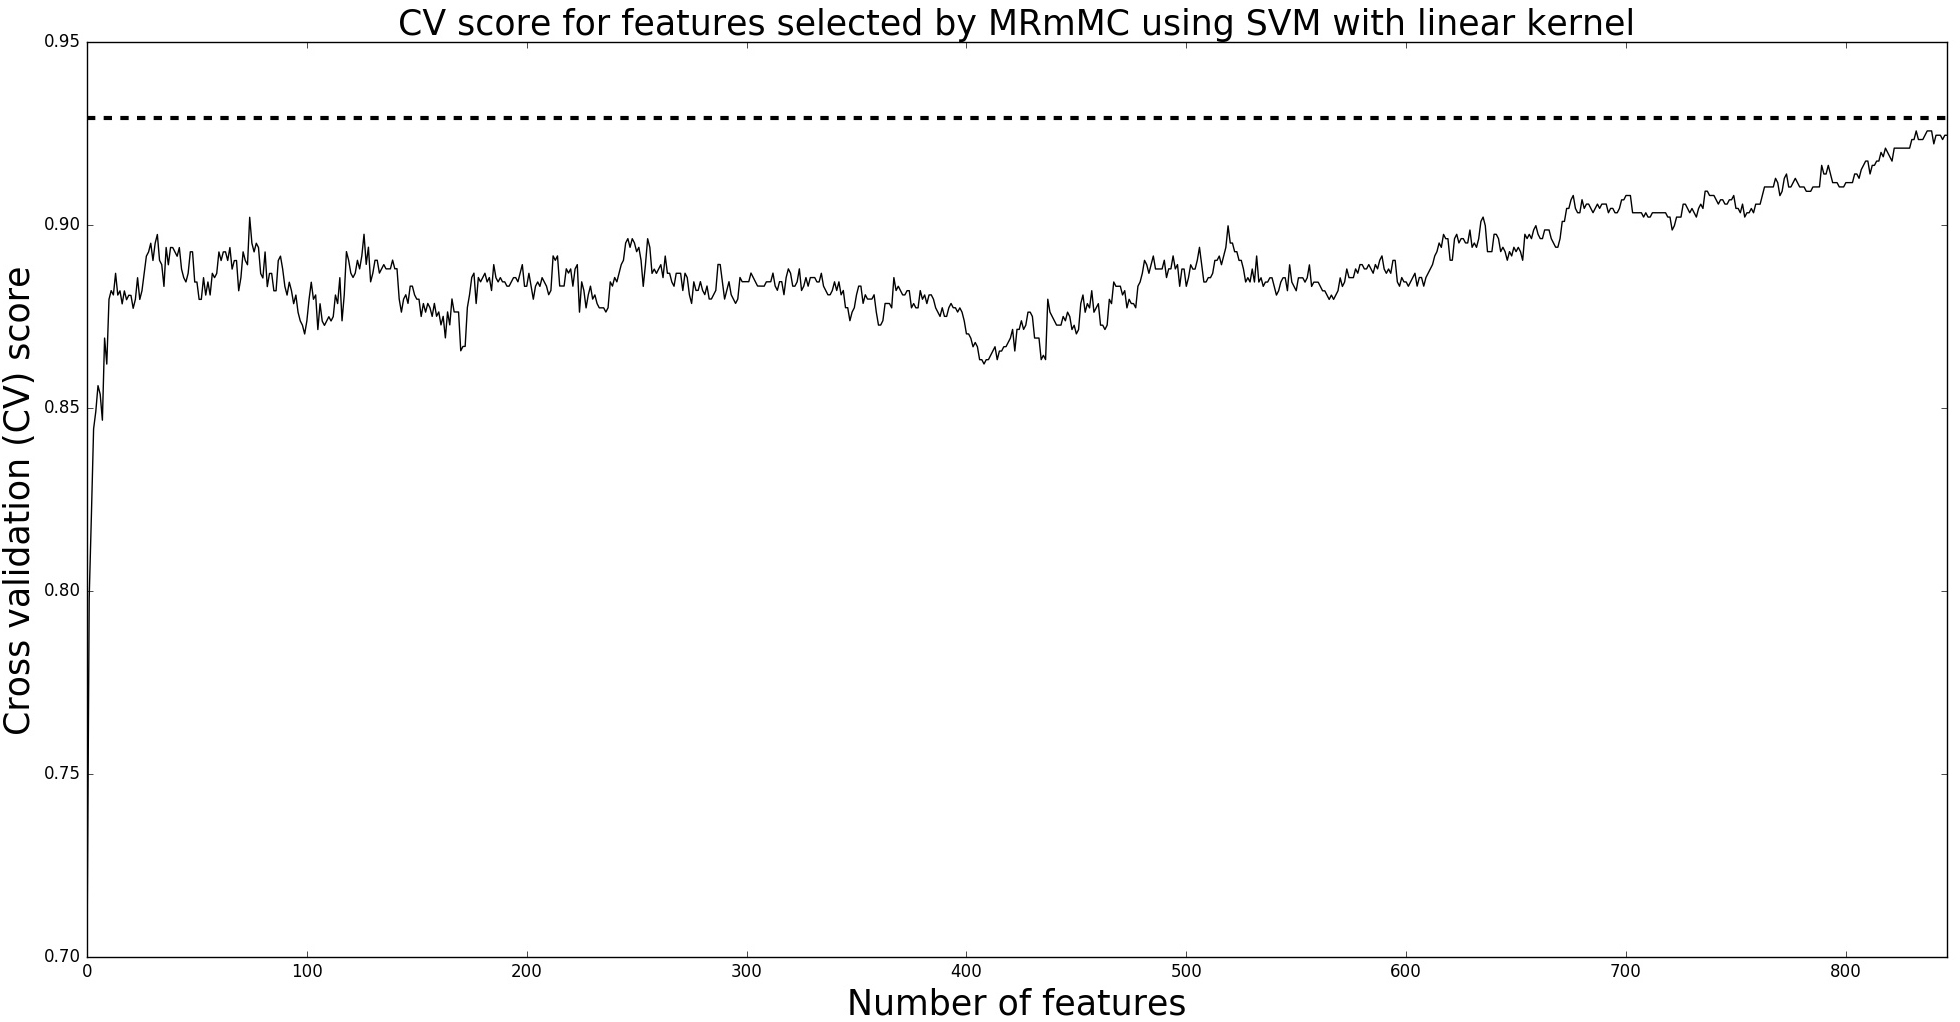
\includegraphics[width=\textwidth]{images/mrmmc_linear_847.jpeg}
\caption{A graph of CV scores against number of features using the full version of MRmMC.}
\label{body:mrmmc:graph}
\end{figure}

\section{MRmMC}

As mentioned in section \ref{mrmmc_probs}, the MRmMC method only allows us to expand our feature subset $S$ until $|S|=847$. We present plots of the CV scores obtained based on the features selected by both the truncated (Figure \ref{body:mrmmc_trun}) and full (Figure \ref{body:mrmmc:graph}) versions of MRmMC. The CV scores presented in this section allow us to compare the effectiveness of incorporating GAs with MRmMC.

\subsection{Comparison between truncated and full versions of MRmMC}

The truncated version of MRmMC emulates RFS in that it only considers features that have high correlation coefficient $r_{qn}$, whereas the full version of the algorithm will consider all features that have not been selected. We will thus expect the truncated version to suffer in optimality.

However, what we see from Figures \ref{body:mrmmc_trun} and \ref{body:mrmmc:graph} is that the truncated version is able to find a feature subset $S$ that can perform better than that found in the full version. For the full version of MRmMC, the CV score peaks at $k=41$ with a CV score of 0.911408. For the truncated version of MRmMC, the CV score peaks at $k=832$ with a score of 0.925603. Thus, interestingly, the truncated version performs better than the full version \textit{within this range of $k$}. We cannot make conclusions about values of $k$ beyond this range.


\subsection{Limitation of MRmMC}

Evidently from both graphs, we can see that there is a general increasing trend in CV score as the number of features $k$ increases, but both methods are not able to find features that can do better than the threshold. Had the algorithm allowed more features to be included in the set, we might obtain a feature subset $S$ that can do better than the threshold.

However, we can also argue that we just require the CV score of $S$ to be within a \textit{range} of the threshold CV score. For example, we might just need the CV score of $S$ to be within 5\% of the threshold. This means that the minimum CV score that we can accept is 0.882702, which is 95\% of the threshold CV score of 0.929160. Both the full and truncated versions satisfy this constraint.

Furthermore, previous methods, such as $t$-test, give us an approximate idea of the size of $S$ that will give us better performance than the threshold. $S$ should contain at least about 2000 features. Thus, we will not expect the subset that MRmMC chooses to outperform the set with all of the available features, since MRmMC can only choose 847 features from the data set. This is evident from the plots above.

%For example, in the truncated version (Figure \ref{body:mrmmc_trun}), the CV scores exhibit an increasing trend, but does not cross the dotted horizontal line that represents the full feature set.


\section{MRmMC with Genetic Algorithm} \label{mrmmc_ga_results}

Here, we modify MRmMC by removing the computation of $R^2$ and incorporating a genetic algorithm (GA). We also experiment with two selection strategies. Since the algorithm contains probabilistic elements, such as the mutation operator, the algorithm was run several times, and the average was taken. 10 runs were performed for each experimental setting. To obtain more accurate averages, we could perform more runs.

For these experiments, the number of features selected for the \textit{first generation} of the GA, $k$ is 8000, as illustrated in Figure \ref{bg:ga:twostage_b}. We differentiate this value of $k$ from the number of features eventually chosen by the algorithm in the subset $S$. We also select 16000 features that have the highest $r_{qn}$ measure for the \textit{first stage} of the GA, as illustrated in Figure \ref{bg:ga:twostage_a}.

\subsection{Roulette Wheel}

First, Algorithm \ref{GAAlgo} was implemented with the Roulette Wheel seletion strategy. The parameters of the GA are listed in Table \ref{ga:mrmmc:params_1}.  The results obtained from the 10 runs were:
\begin{center}
    \begin{tabular}{| c | c | c | c | } \hline
    Run & CV score & Number of iterations & Number of features chosen \\ \hline \hline
    1 & 0.9551 & 6 & 8102 \\ \hline
	2 & 0.9587 & 8 & 8070 \\ \hline
	3 & 0.9563 & 9 & 7977 \\ \hline
	4 & 0.9563 & 6 & 8024 \\ \hline
	5 & 0.9586 & 6 & 7960 \\ \hline
	6 & 0.9563 & 7 & 8046 \\ \hline
	7 & 0.9586 & 7 & 8007 \\ \hline
	8 & 0.9551 & 10 & 7960 \\ \hline
	9 & 0.9563 & 10 & 7988 \\ \hline
	10 & 0.9575 & 8 & 7999 \\ \hline
	Average & 0.9569 & 7.7 & 8013.3 \\ \hline
    \end{tabular}
\end{center}

On average, we see that the CV score is approximately 0.9569, slightly better than $t$-test in section \ref{t-test}. However, we note that in $t$-test, the best score of 0.950 was obtained with 15000 features, compared to about 8000 features with the GA, which is half of that in $t$-test. Furthermore, as the \textit{elitism strategy} was implemented, the number of iterations required by the GA is relatively low, as the CV score for each generation is guaranteed to be non-decreasing.

\begin{table}
\begin{center}
    \begin{tabular}{| p{12cm} | c |} \hline
    Parameters & Value \\ \hline \hline
    Number of features selected in first stage of GA $k$ & 8000 \\ \hline
    Number of top features to select with respect to $r_{qn}$ heuristic in first stage of GA $s$ & 16000 \\ \hline
    Number of solutions in each generation $G$ & 50 \\ \hline
    Threshold number of generations to terminate algorithm $T$ & 5 \\ \hline
    Mutation rate $p_m$ &  0.05 \\ \hline
    ``Runner-up'' solutions to be chosen for mutation $p_r$ & 0.05 \\ \hline
    Cloning/elitism rate $p_e$ & 0.05 \\ \hline
    Rate of eliminating solutions with worst fitness $p_{elim}$ & 0.05 \\ \hline
    Number of solutions in tournament for tournament selection $N_t$ & 2 \\ \hline
    Probability of choosing winner in tournament selection $p_t$ & 0.8 \\ \hline
    Termination threshold for fitness $t$ & 0.001 \\ \hline
    \end{tabular}
\end{center}
\caption{Table of parameters used in genetic algorithm implementation of MRmMC.}
\label{ga:mrmmc:params_1}
\end{table}

We also note that the final number of features chosen by the GA is also roughly similar to the value $k$ that we provide for the algorithm. We investigate if changing $k$ drastically will make a difference to the outcome. To this end, we also set $k=10,50,100$, while keeping the rest of the parameters the same as in Table \ref{ga:mrmmc:params_1}.

For $k=100$:

\begin{center}
    \begin{tabular}{| c | c | c | c | } \hline
    Run & CV score & Number of iterations & Number of features chosen \\ \hline \hline
    1 & 0.9610 & 19 & 7350 \\ \hline
	2 & 0.9598  & 16 & 6628 \\ \hline
	3 & 0.9563 & 14 & 6587 \\ \hline
	4 & 0.9563 & 18 & 7563 \\ \hline
	5 & 0.9563 & 19 & 7464 \\ \hline
	6 & 0.9563 & 22 & 7588 \\ \hline
	7 & 0.9551 & 15 & 6610 \\ \hline
	8 & 0.9563 & 15 & 6745 \\ \hline
	9 & 0.9575 & 14 & 6469 \\ \hline
	10 & 0.9587 & 22 & 7654 \\ \hline
	Average & 0.9574 & 17.4 & 7065.8 \\ \hline
    \end{tabular}
\end{center}

For $k=50$:

\begin{center}
    \begin{tabular}{| c | c | c | c | } \hline
    Run & CV score & Number of iterations & Number of features chosen \\ \hline \hline
    1 & 0.9575 & 15 & 6523 \\ \hline
	2 & 0.9586  & 15 & 6232 \\ \hline
	3 & 0.9551 & 11 & 4523 \\ \hline
	4 & 0.9539 & 14 & 6269 \\ \hline
	5 & 0.9563 & 14 & 6413 \\ \hline
	6 & 0.9586 & 19 & 7260 \\ \hline
	7 & 0.9598 & 16 & 6600 \\ \hline
	8 & 0.9575 & 14 & 6563 \\ \hline
	9 & 0.9563 & 15 & 6758 \\ \hline
	10 & 0.9539 & 18 & 7303 \\ \hline
	Average & 0.9564 & 15.1 & 6482.9 \\ \hline
    \end{tabular}
\end{center}


For $k=10$:

\begin{center}
    \begin{tabular}{| c | c | c | c | } \hline
    Run & CV score & Number of iterations & Number of features chosen \\ \hline \hline
    1 & 0.9563 & 16 & 6810 \\ \hline
	2 & 0.9586  & 19 & 7314 \\ \hline
	3 & 0.9574 & 17 & 6880 \\ \hline
	4 & 0.9539 & 17 & 7199 \\ \hline
	5 & 0.9551 & 12 & 4424 \\ \hline
	6 & 0.9551 & 9 & 4036 \\ \hline
	7 & 0.9575 & 11 & 5357 \\ \hline
	8 & 0.9574 & 20 & 6427 \\ \hline
	9 & 0.9575 & 14 & 7072 \\ \hline
	10 & 0.9563 & 17 & 7096 \\ \hline
	Average & 0.9565 & 15.2 & 6261.5 \\ \hline
    \end{tabular}
\end{center}

We see that despite reducing $k$ drastically, on average, the final number of features selected by the algorithm still remains in the thousands. Interestingly, for $k=10$, the final number of features chosen is the lowest among the three experiments. The case of $k=100$ also achieved the highest CV score so far of 0.9610.

\subsection{Tournament selection}

Here, we change the selection strategy to tournament selection, and construct similar tables to those in the previous section.

For $k=8000$,
\begin{center}
    \begin{tabular}{| c | c | c | c | } \hline
    Run & CV score & Number of iterations & Number of features chosen \\ \hline \hline
    1 & 0.9599 & 15 & 8085 \\ \hline
	2 & 0.9575  & 7 & 8090 \\ \hline
	3 & 0.9598 & 15 & 7967 \\ \hline
	4 & 0.9575 & 6 & 7966 \\ \hline
	5 & 0.9563 & 7 & 7991 \\ \hline
	6 & 0.9575 & 5 & 8000 \\ \hline
	7 & 0.9610 & 14 & 8038 \\ \hline
	8 & 0.9563 & 11 & 8021 \\ \hline
	9 & 0.9610 & 10 & 7956 \\ \hline
	10 & 0.9610 & 11 & 7936 \\ \hline
	Average & 0.9587 & 10.1 & 8005 \\ \hline
    \end{tabular}
\end{center}

For $k=100$,
\begin{center}
    \begin{tabular}{| c | c | c | c | } \hline
    Run & CV score & Number of iterations & Number of features chosen \\ \hline \hline
    1 & 0.9598 & 18 & 7356 \\ \hline
	2 & 0.9563  & 15 & 6981 \\ \hline
	3 & 0.9575 & 14 & 6558 \\ \hline
	4 & 0.9587 & 11 & 6094 \\ \hline
	5 & 0.9563 & 11 & 5588 \\ \hline
	6 & 0.9586 & 15 & 7373 \\ \hline
	7 & 0.9587 & 11 & 5783 \\ \hline
	8 & 0.9575 & 14 & 5574 \\ \hline
	9 & 0.9622 & 19 & 7615 \\ \hline
	10 & 0.9634 & 17 & 7341 \\ \hline
	Average & 0.9589 & 14.5 & 6626.3 \\ \hline
    \end{tabular}
\end{center}


For $k=50$,
\begin{center}
    \begin{tabular}{| c | c | c | c | } \hline
    Run & CV score & Number of iterations & Number of features chosen \\ \hline \hline
    1 & 0.9586 & 17 & 7492 \\ \hline
	2 & 0.9633 & 16 & 7042 \\ \hline
	3 & 0.9575 & 17 & 7623 \\ \hline
	4 & 0.9563 & 17 & 7667 \\ \hline
	5 & 0.9610 & 15 & 6925 \\ \hline
	6 & 0.9610 & 12 & 5746 \\ \hline
	7 & 0.9586 & 14 & 6911 \\ \hline
	8 & 0.9586 & 16 & 7339 \\ \hline
	9 & 0.9563 & 15 & 6917 \\ \hline
	10 & 0.9575 & 14 & 6285 \\ \hline
	Average & 0.9589 & 15.3 & 6994.7 \\ \hline
    \end{tabular}
\end{center}

For $k=10$,
\begin{center}
    \begin{tabular}{| c | c | c | c | } \hline
    Run & CV score & Number of iterations & Number of features chosen \\ \hline \hline
    1 & 0.9563 & 16 & 6810 \\ \hline
	2 & 0.9586 & 19 & 7314 \\ \hline
	3 & 0.9574 & 17 & 6880 \\ \hline
	4 & 0.9539 & 17 & 7199 \\ \hline
	5 & 0.9551 & 12 & 4424 \\ \hline
	6 & 0.9551 & 9 & 4036 \\ \hline
	7 & 0.9575 & 11 & 5357 \\ \hline
	8 & 0.9574 & 20 & 6427 \\ \hline
	9 & 0.9575 & 14 & 7072 \\ \hline
	10 & 0.9565 & 17 & 7096 \\ \hline
	Average & 0.9589 & 15.2 & 6261.5 \\ \hline
    \end{tabular}
\end{center}


\subsection{Effects of $k$}
Overall, we see that on average, the CV score, number of iterations and number of features chosen by the algorithm, do not change drastically with $k$. This seems to apply for both selection strategies. For all of the above settings, the CV scores fall between 0.95 and 0.96, the number of iterations rarely exceeds 20, and the number of features chosen by the GA is between 4000 to about 8000, regardless of the selection strategy and $k$.

\subsection{Redundancy in genetic algorithm}

In general, we see that the GA does not require many iterations to converge for this data set, and its CV scores are similar compared to $t$-test at about 0.95. At the same time, we see that for similar CV scores, the GA is able to form a subset that is much smaller than that produced by the $t$-test.

The GA was proposed to eliminate the need to compute $R^2$, but the problem of redundancy still arises in the GA, since we do not use a specific measure to quantify redundancy among the selected features. We might argue that for a CV score of about 0.95, the number of features selected by the GA is about half of those selected by $t$-test. We might have removed some redundancy from the features in $t$-test, but we cannot be absolutely certain, unless we explicitly check if each feature in the subset is redundant with respect to the other features.

This is proposed as an extension in section \ref{further_work}.

\subsection{Evaluation of two-stage genetic algorithm}

In the GA, we have employed the two-stage GA as discussed in section \ref{bg:ga:twostage}. The first stage calculates the $r_{qn}$ quantity as specified in the MRmMC paper in \cite{RefWorks:187} and chooses only the top 16000 features (Figure \ref{ga:mrmmc:params_1}) that have the highest $r_{qn}$. We see that considering only features that have the best individual $r_{qn}$ values does not seem to degrade the performance of the algorithm significantly, as indicated by the CV scores.

This has also allowed the algorithm to reduce the amount of memory needed, since we only need to keep track of the top 16000 features, instead of considering all 420374 features. Evidently, this is another parameter that can vary. We might be able to save even more memory by filtering out more features in the first stage of the GA. At the same time, we might also have missed out important features by truncating those features that do not have high $r_{qn}$. This issue will require further investigation into the parameters of the GA, as discussed in section \ref{further_work}.


%\section{Summary of methods}

%We present a table that summarises the methods and results that have been presented in the previous sections.

%\subsection{Trade-offs}

%Firstly, it is interesting to see that the performance of $t$-test peaks with almost the same level of accuracy as the GAs, although it chooses a much higher number of features. In fact, the $t$-test selects almost twice as many features as the GAs. This relates back to section \ref{t_test:redundancy}, where it was mentioned that the $t$-test does not take into account redundancy of the features. In particular, the top 15000 features selected by $t$-test might contain redundant features.

%Secondly, even though the MRmMC method is a filter method, since it does not employ the SVM, the algorithm is slowed down by the computation of orthogonal vectors which was needed to quantify redundancy.

\section{Biological interpretation} \label{bio:conclusion}

In this section, we attempt to see if there are any features that repeatedly get selected by the feature selection algorithms. In particular, we inspect the features that are chosen in the following scenarios:
\begin{itemize}
  \item $t$-test with $k=15000$
  \item MRmMC with $k=41$
  \item Truncated MRmMC with $k=832$
  \item All features selected by MRmMC with GA where the CV score exceeds 0.96. 
\end{itemize}

These settings are selected because the CV scores of the chosen feature subsets are relatively high.

We then see which features, if any, are selected in all or most of the above scenarios. To do this, we  keep track of an array of 420374 zeros, and then count the number of times each feature appears in the above settings. In all of the experiments listed in this chapter, the features in the data set are represented by \textit{indices}. So, if the algorithm selects a feature with index 50, we can find the feature by simply getting the 50th column of the data set.

We find that in out of the 9 settings listed above, the feature \texttt{cg13055685} appears in all 9 settings, 11 features appear in 8 of the settings and 138 features appear in 7 of the settings.

The features that are frequently selected can be mapped to a database that is publicly available. In particular, we extract information about our features through a database that contains methylation data in humans \cite{bio_conclusion}. From this database, we can extract the features' gene names.

\texttt{cg13055685} corresponds to the gene name \texttt{MCF2L;MCF2L} and the 11 features that appear in 8 of the settings correspond to:
\begin{itemize}
  \item \texttt{MAN2B2}
  \item \texttt{DAXX;DAXX;DAXX;DAXX}
  \item \texttt{SURF2}
  \item \texttt{SCAPER}
  \item \texttt{VPS53;VPS53}
  \item \texttt{MYH7B}
  \item \texttt{CENPL;CENPL;CENPL;CENPL;DARS2;CENPL}
  \item \texttt{MCF2L;MCF2L}
  \item \texttt{DISP2}
  \item \texttt{CHERP}
\end{itemize}

This discovery is made possible with the help of Dr. Karim Malki, who has also been giving advice for this project. At the time of writing, he is investigating the significance, if any, of the above genes.


\chapter{Conclusion}
% The project's conclusions should list the things which have been learnt as a result of the work you have done.
% For example, "The use of overloading in C++ provides a very elegant mechanism for transparent parallelisation of sequential programs"

Overall, this project has explored the epigenetics data collected in \cite{RefWorks:78}. It has also experimented with various feature selection algorithms and investigated the efficacy of these algorithms on the epigenetics data. In particular, we put our focus on the MRmMC algorithm and pointed out some characteristics which might not be applicable to our epigenetics data set. To mitigate these shortcomings, we have also extended the MRmMC algorithm with genetic algorithms under different experimental settings.

We can draw the following conclusions based on the work done in this project:
\begin{itemize}
  \item The $t$-test method is able to select features that give good cross validation scores. Due to its limitations, these features might contain redundancies.
  \item Recursive Feature Elimination requires more fine-tuning in its parameters for it to be effective on the data set.
  \item MRmMC is not suitable for high dimensional data, specifically data with more features than samples.
  \item Incorporating genetic algorithms with MRmMC allowed us to find features that perform slightly better than those found by $t$-test and RFE. It has also allowed us to significantly reduce the number of features obtained.
  \item A way to measure redundancy is still lacking in the GA variant of MRmMC.
  \item Several features were repeatedly selected by the algorithms, and their corresponding genes were obtained.
\end{itemize}

\section{Further work} \label{further_work}

%\subsection{Finding global optima}

One dilemma of greedy feature selection algorithms is that these algorithms only explore a subspace of the feature space, although they can find a local optimum in a shorter time than exhaustive algorithms.

%Most of these algorithms also prune and halt their search if, for example, the performance of a subset starts to decline.

Even though we have shown that some of the algorithms described here can find a subset $S$ that performs better than the full set of features, we are not guaranteed the global optimum. In other words, even though we have found $S$ that can perform better than the full set of features, we do not know if there are other subsets that can perform even better.

The following extensions might help to enhance the performance of the algorithms discussed in this project.

%Thus, an extension might entail a more thorough search of the feature space. Alternatively, a more theoretical approach can be taken, where we might derive upper and lower bounds for the subsets.

\subsection{Using different kernels and classifiers}

In this project, we have limited ourselves to only the SVM. The kernel for the SVM was also mostly linear.

We can explore the effectiveness of using other types of kernels, such as the RBF kernel and the polynomial kernel. We can also try using other classifiers, as doing so might give us more insight into the data. 

\subsection{Exploring parameters and strategies}

Parameters play an important role in feature selection algorithms. One of such parameters is the value of $k$, the number of features to be selected from the set of features.

The number of parameters and strategies also increases in GAs. As mentioned in section \ref{bg:fs:ga}, there are many parameters in GAs that need to be tuned, and it might be instructive to experiment with parameters that are different from the ones used in this project. However, this might involve optimisation in many dimensions, where each dimension represents a parameter. Furthermore, different strategies can be used in GAs, such as different terminating conditions, crossover, selection and mutation strategies.

Thus, further work in this aspect will involve finding optimum parameters and/or strategies that can improve the search over the feature space.


\subsection{Use of mutual information} \label{extension:mi}
As mentioned in section \ref{bg:fs:mi}, mutual information (MI) is a highly popular measure to quantify the relationship between features and the target class (relevance) and between features themselves (redundancy). MI has also been used in many other works involving feature selection.

This project avoids the use of MI despite its popularity, simply because the data set uses continuous variables. MI also requires estimates of probabilities and it is computationally complex to estimate probabilities involving continuous variables.

Various methods have been proposed to estimate MI for continuous variables. For example, the Parzen Window \cite{RefWorks:183} was proposed to estimate these probabilities. An extension can make use of the Parzen Window method to help estimate probabilities involving continuous variables. Parameters of the Parzen Window method also need to be optimised. This can then be combined with the algorithms used in this project. We can then determine if using the Parzen Window (or other methods) to estimate MI improves the feature selection process.


\subsection{Quantifying redundancy in MRmMC}

Although implementing a GA with MRmMC gave good cross validation scores with a relatively small number of features, we cannot be sure if the features chosen contain any redundancy. An extension can thus be to check for redundancy within this chosen set of features.

The authors of the MRmMC paper in \cite{RefWorks:187} also suggested the need for an alternative redundancy measure. This might be due to the limitations of the redundancy measure $R^2$ that was originally proposed.

Suppose we are successful in estimating probabilities of continuous variables using mutual information as suggested in section \ref{extension:mi}, we can use the redundancy measure discussed in section \ref{bg:fs:mi}:
\begin{align*}
\min \, R(S) = \frac{1}{|S|^2} \sum_{x_i, x_j \in S} I(x_i, x_j)
\end{align*}

This measure was originally proposed in \cite{RefWorks:182}.


\subsection{Further metrics to evaluate algorithms}

From section \ref{mrmmc_ga_results}, the quantities listed in tables - best cross validation (CV) score, number of iterations and number of features chosen - can be used to evaluate the efficiency and efficacy of feature selection algorithms. In the previous chapter, we have evaluated the performance of the subset $S$ based on CV scores. An alternative will be to consider the above quantities to evaluate $S$.

For example, we can propose a metric $J$ to select a subset $\widehat{S}$ that takes into account the CV score $C$, the number of iterations $I$, and the number of features chosen $F$. Intuitively, we maximise $C$ and minimise $I$ and $F$. That is,
\begin{align*}
\widehat{S} = \argmax \, J(S) = C - I - F
\end{align*}

We can also decide to weigh $C$, $I$ and $F$ with non-negative coefficients:
\begin{align*}
\widehat{S} = \argmax \, J(S) = \alpha C - \beta I - \gamma F
\end{align*}
where $\alpha, \beta, \gamma \in \mathbb{R}$. This is similar to the fitness function used in \cite{RefWorks:199}.

An extension will thus use this metric to evaluate $S$, not just based on its CV score.

\newpage

\singlespacing
\pagenumbering{roman}

\bibliographystyle{unsrt}
\bibliography{references}

\end{document}